%% Generado por html2tex.py desde temas.json (bio). No editar a mano: corregir la clase en el .js del sitio y regenerar.
\parteciencia{bio}
\chapter{Organización celular}
%% =====================================================================
%% bio_celulas
\section[Células procariontes y eucariontes]{Células procariontes y eucariontes}
\modcomun\ \ {\color{gris}\itshape La teoría celular, cómo son las células procariontes y eucariontes y qué estructuras tienen las células animales y vegetales: cápsula, pared celular, membrana, citoplasma, núcleo, ribosomas, cloroplastos y vacuola central.\par}
\subsection{La teoría celular}
En 1665, Robert Hooke miró una lámina de corcho con un microscopio sencillo y vio pequeñas cavidades que llamó \textbf{células}. Pocos años después, Anton van Leeuwenhoek, con lentes mejores, observó por primera vez organismos unicelulares vivos en gotas de agua.

 

Durante el siglo XIX, con microscopios más potentes, se reunieron las observaciones en la \textbf{teoría celular}:

 
\begin{itemize}
  \item \textbf{Todos los seres vivos están formados por una o más células} (Schleiden en plantas, 1838; Schwann en animales, 1839).
  \item \textbf{La célula es la unidad estructural y funcional} de los seres vivos: es la estructura más pequeña que cumple todas las funciones vitales.
  \item \textbf{Toda célula proviene de otra célula preexistente}, por división (Virchow, 1855).
  \item La célula contiene la \textbf{información hereditaria} (ADN), que pasa a las células hijas.
\end{itemize}
  
\begin{clave}[{Por qué tardó tanto}] Casi todas las células miden entre 1 y 100 µm (micrómetros), muy por debajo de lo que distingue el ojo (unos 100 µm). La teoría celular dependió del avance de la \textbf{microscopía}: sin lentes de buena calidad no había cómo observar ni comparar células.\end{clave}
 
\begin{ejemplo}[{Ejemplo resuelto}] En un cultivo, cada célula nueva aparece siempre por la división de una célula que ya existía; nunca a partir de materia sin vida. Esta observación apoya el postulado «toda célula proviene de otra célula preexistente».\end{ejemplo}
\subsection{Células procariontes}
Las \textbf{procariontes} (bacterias y arqueas) son las células más simples y pequeñas (1 a 10 µm). Su rasgo central: \textbf{no tienen núcleo}. Su ADN es una molécula circular que está en una zona del citoplasma llamada \textbf{nucleoide}. Tampoco tienen organelos rodeados por membrana.

 
\begin{itemize}
  \item \textbf{Membrana plasmática:} bicapa de fosfolípidos que regula qué entra y qué sale.
  \item \textbf{Pared celular:} capa rígida por fuera de la membrana; en las bacterias está hecha de \textbf{peptidoglicano}. Da forma y evita que la célula estalle al entrar agua. La penicilina actúa impidiendo su formación.
  \item \textbf{Cápsula:} capa externa de polisacáridos, presente en algunas bacterias. Las ayuda a adherirse a superficies y a evitar ser fagocitadas por los glóbulos blancos.
  \item \textbf{Ribosomas:} fabrican las proteínas (en bacterias son más pequeños que en eucariontes).
  \item \textbf{Plásmidos:} pequeñas moléculas de ADN circular extra, con genes como los de resistencia a antibióticos.
  \item \textbf{Flagelo} (movimiento) y \textbf{pili} (adherencia e intercambio de ADN).
\end{itemize}
  
\begin{center}
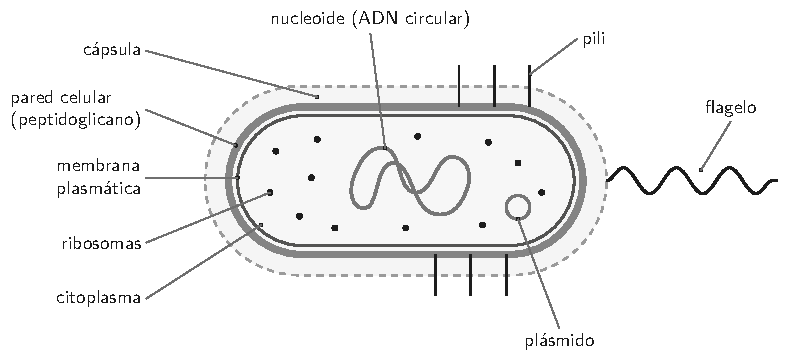
\includegraphics[max width=0.92\linewidth,max height=8.5cm]{bio/cel_procarionte}
\end{center}
\subsection{Células eucariontes}
Las \textbf{eucariontes} forman a los protistas, hongos, plantas y animales. Son más grandes (10 a 100 µm) y más complejas:

 
\begin{itemize}
  \item Tienen \textbf{núcleo}: el ADN está dentro de una envoltura de doble membrana con poros.
  \item Tienen \textbf{organelos rodeados por membrana}, cada uno con su tarea: retículo endoplasmático, complejo de Golgi, lisosomas, mitocondrias, cloroplastos (en plantas y algas), vacuolas.
  \item Tienen \textbf{citoesqueleto}, una red de filamentos de proteína que da forma, mueve organelos y permite el movimiento celular.
  \item Su ADN es lineal, está asociado a proteínas (histonas) y repartido en varios cromosomas.
\end{itemize}
 

Esta división del trabajo en compartimentos permite que en una misma célula ocurran a la vez procesos que necesitan condiciones distintas, como la digestión ácida en los lisosomas y la síntesis de proteínas en el citoplasma.

  
\begin{clave}[{La teoría endosimbiótica}] Lynn Margulis propuso que las \textbf{mitocondrias} y los \textbf{cloroplastos} fueron procariontes que otra célula incorporó sin digerirlos. Evidencias: tienen \textbf{doble membrana}, \textbf{ADN circular propio}, \textbf{ribosomas parecidos a los bacterianos} y se reproducen por \textbf{división} dentro de la célula.\end{clave}
\subsection{Célula animal y célula vegetal}
\begin{center}
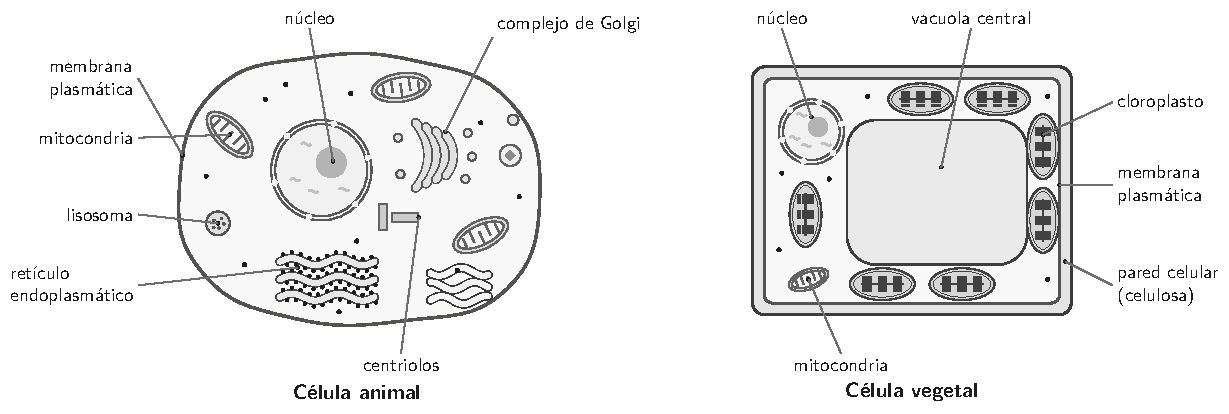
\includegraphics[max width=0.92\linewidth,max height=8.5cm]{bio/cel_animal_vegetal}
\end{center}
  

\textbf{Solo en la célula vegetal} (típica de una hoja):

 
\begin{itemize}
  \item \textbf{Pared celular de celulosa:} rígida, da forma y resiste la presión del agua.
  \item \textbf{Cloroplastos:} realizan la fotosíntesis.
  \item \textbf{Vacuola central grande:} guarda agua, iones y pigmentos; al llenarse empuja contra la pared y mantiene la célula firme (turgencia).
\end{itemize}
  

\textbf{Solo en la célula animal:}

 
\begin{itemize}
  \item \textbf{Centriolos} (las plantas con flor no los tienen).
  \item \textbf{Lisosomas} típicos; en las plantas, la vacuola cumple parte de la función digestiva.
  \item Forma variable, porque no hay pared.
\end{itemize}
 

\textbf{En ambas:} membrana plasmática, citoplasma, núcleo, ribosomas, retículo endoplasmático, complejo de Golgi y \textbf{mitocondrias}. Las plantas también respiran.
\subsection{Lo clave del tema}
\begin{center}\small
\begin{tabularx}{\linewidth}{@{}>{\raggedright\arraybackslash\hsize=0.87\hsize}X>{\raggedright\arraybackslash\hsize=1.20\hsize}X>{\raggedright\arraybackslash\hsize=0.93\hsize}X@{}}
\toprule
\textbf{Estructura} & \textbf{Función} & \textbf{Dónde está} \\
\midrule
Cápsula & adherencia; evitar la fagocitosis & algunas bacterias \\
Pared celular & forma y resistencia a la presión del agua & bacterias, hongos, plantas \\
Membrana plasmática & límite celular; regula el paso de sustancias & todas las células \\
Ribosomas & síntesis de proteínas & todas las células \\
Núcleo & guarda el ADN y controla la célula & eucariontes \\
Flagelo & movimiento & bacterias y algunas eucariontes \\
Cloroplasto / vacuola central & fotosíntesis / agua, reservas y turgencia & células vegetales \\
\bottomrule
\end{tabularx}
\end{center}
 
\begin{clave}[{Recuerda}] · Procarionte = sin núcleo y sin organelos membranosos; su ADN circular está en el nucleoide.\par · Las plantas tienen mitocondrias además de cloroplastos.\par · La pared bacteriana es de peptidoglicano; la vegetal, de celulosa.\par · Mitocondrias y cloroplastos tienen ADN propio y doble membrana: evidencia de la endosimbiosis.\end{clave}
 
\begin{clave}[{Método PAES}] 1. Si te preguntan por una estructura bacteriana, relaciona la función descrita (moverse, adherirse, resistir la fagocitosis, resistir la presión) con flagelo, pili, cápsula o pared. 2. En una célula vegetal, une el agua, los pigmentos y la turgencia con la vacuola central, y la fotosíntesis con los cloroplastos. 3. En preguntas de historia de la ciencia, relaciona cada observación con el postulado de la teoría celular que apoya y recuerda que todo dependió de la microscopía.\end{clave}
\begin{elejemplo}{PAES Invierno 2026, adaptada}
Unos microbiólogos estudian bacterias que nadan hacia las zonas del medio de cultivo donde hay más nutrientes. Obtienen una cepa mutante que crece y se divide con normalidad, pero que ya no logra desplazarse en el líquido: queda siempre en el mismo lugar donde se sembró.

¿Qué estructura bacteriana está alterada con mayor probabilidad en la cepa mutante?
\alts{La cápsula.}{El flagelo.}{El plásmido.}{Los ribosomas.}
\solucion{\textbf{Paso 1. ¿Qué nos piden?} La estructura relacionada con la función que se perdió: \textbf{desplazarse en un líquido}.

\textbf{Paso 2. Relaciona función y estructura.} En las bacterias, el movimiento en medios líquidos depende del \textbf{flagelo}, un filamento largo que gira como una hélice y empuja a la célula.

\textbf{Paso 3. Usa el resto de la información.} La mutante crece y se divide normal: su metabolismo, su ADN y su síntesis de proteínas funcionan. Solo perdió la movilidad.

\textbf{Respuesta:} el flagelo.

\textbf{¿Por qué no las otras?} La cápsula sirve para adherirse y evitar la fagocitosis, no para nadar. Los plásmidos llevan genes extra (por ejemplo, de resistencia a antibióticos). Si los ribosomas fallaran, la bacteria no podría fabricar proteínas y no crecería con normalidad.

\textbf{\color{cienciaD}Para recordar.} Moverse en un líquido: flagelo.}{B}
\end{elejemplo}
\motivacion{Toda vida empieza con una célula, y todo buen puntaje empieza con un tema. Ya diste el primer paso.}

%% =====================================================================
%% bio_organelos
\section[Organelos y estructuras celulares]{Organelos y estructuras celulares}
\modcomun\ \ {\color{gris}\itshape Estructura y función de membrana, citoesqueleto, núcleo, nucléolo, ribosomas, retículos endoplasmáticos, complejo de Golgi, lisosomas, peroxisomas, mitocondrias, cloroplastos, vacuolas, centriolos, cilios y flagelos; la ruta de síntesis y secreción de proteínas y cómo se estudia con marcaje radiactivo y organelos inhibidos.\par}
\subsection{Mapa de la célula eucarionte}
\begin{center}
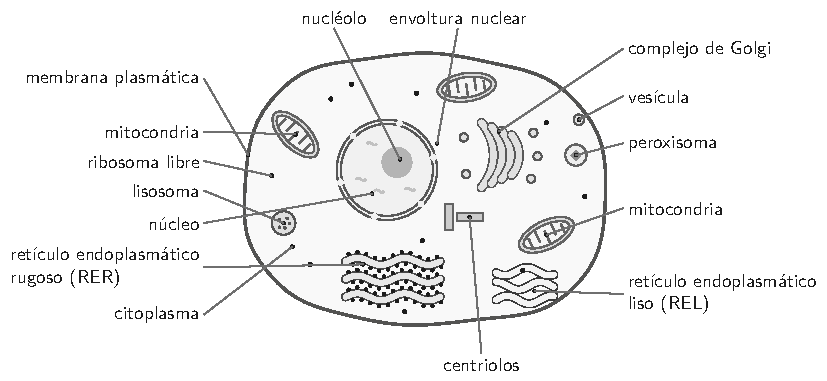
\includegraphics[max width=0.92\linewidth,max height=8.5cm]{bio/cel_organelos}
\end{center}
  

\textbf{Membrana plasmática.} Bicapa de fosfolípidos con proteínas y colesterol (en animales). Es \textbf{semipermeable}: deja pasar con facilidad algunas sustancias (O\textsubscript{2}, CO\textsubscript{2}, agua) y regula el paso de otras con proteínas transportadoras. Sus glicoproteínas permiten que las células se reconozcan.

  

\textbf{Organelos con membrana}: núcleo, retículos, Golgi, lisosomas, peroxisomas, vacuolas, mitocondrias y cloroplastos. \textbf{Estructuras sin membrana}: ribosomas, citoesqueleto, centriolos y nucléolo.

 

Tienen \textbf{doble membrana} el núcleo (envoltura nuclear), las mitocondrias y los cloroplastos.
\subsection{Citoesqueleto, centriolos, cilios y flagelos}
El \textbf{citoesqueleto} es una red de filamentos de proteína que recorre el citoplasma. Da forma a la célula, la hace resistente a fuerzas mecánicas, mueve los organelos y permite que la célula se desplace. Tiene tres tipos de filamentos:

 
\begin{itemize}
  \item \textbf{Microfilamentos} (actina): cambios de forma, emisión de pseudópodos, contracción muscular, división del citoplasma; sostienen las microvellosidades.
  \item \textbf{Filamentos intermedios} (como la queratina): resistencia a la tensión mecánica.
  \item \textbf{Microtúbulos} (tubulina): «rieles» por los que viajan vesículas y organelos; forman el \textbf{huso mitótico}, los cilios y los flagelos.
\end{itemize}
  

\textbf{Centriolos.} Par de cilindros de microtúbulos, perpendiculares entre sí, en el centrosoma de las células animales. Organizan los microtúbulos, por ejemplo durante la división celular.

 

\textbf{Cilios y flagelos.} Prolongaciones de la membrana con un esqueleto de microtúbulos que se mueven gastando ATP. Los \textbf{cilios} son cortos y numerosos: en la tráquea barren el mucus hacia arriba; en el oviducto mueven al ovocito. El \textbf{flagelo} es largo y suele ser único: mueve al espermatozoide.

 
\begin{clave}[{Recuerda}] Si un fármaco desarma los microtúbulos, se afectan a la vez el transporte de vesículas, la separación de cromosomas en la mitosis y el movimiento de cilios y flagelos.\end{clave}
\subsection{Núcleo, nucléolo y ribosomas}
\textbf{Núcleo.} Guarda el ADN y controla la actividad celular decidiendo qué genes se expresan. Está rodeado por la \textbf{envoltura nuclear}, de doble membrana, con \textbf{poros} por los que salen los ARN y entran proteínas. Dentro, el ADN está unido a proteínas (histonas) formando la \textbf{cromatina}.

 

\textbf{Nucléolo.} Zona del núcleo, sin membrana, donde se fabrica el \textbf{ARN ribosomal} y se arman las \textbf{subunidades de los ribosomas}, que luego salen al citoplasma por los poros. Las células que fabrican muchas proteínas tienen nucléolos grandes.

  

\textbf{Ribosomas.} Estructuras sin membrana, de ARN y proteínas, que \textbf{sintetizan proteínas} leyendo el ARN mensajero. Pueden estar:

 
\begin{itemize}
  \item \textbf{libres en el citoplasma:} hacen proteínas que se quedan en el citoplasma (por ejemplo, enzimas de la glucólisis);
  \item \textbf{adheridos al retículo endoplasmático rugoso:} hacen proteínas que se secretan (enzimas digestivas, hormonas como la insulina, anticuerpos), proteínas de membrana y enzimas de los lisosomas.
\end{itemize}
 
\begin{clave}[{Cadena de efectos}] Si se daña el nucléolo, se forman menos ribosomas; con menos ribosomas, con el tiempo baja la síntesis de proteínas. El efecto \textbf{directo} es el primero.\end{clave}
\subsection{Retículos endoplasmáticos y complejo de Golgi}
\textbf{Retículo endoplasmático rugoso (RER).} Sacos aplanados conectados con la envoltura nuclear y cubiertos de ribosomas. Allí se sintetizan las proteínas de secreción y de membrana; dentro del RER se pliegan y empiezan a modificarse. Luego salen en \textbf{vesículas de transporte} hacia el Golgi.

 

\textbf{Retículo endoplasmático liso (REL).} Túbulos sin ribosomas. Funciones:

 
\begin{itemize}
  \item síntesis de \textbf{lípidos}: fosfolípidos de membrana y \textbf{hormonas esteroidales} (testosterona, estrógenos, cortisol);
  \item \textbf{detoxificación} de fármacos, alcohol y otras sustancias, sobre todo en el hígado;
  \item almacenamiento de \textbf{calcio}: en el músculo se llama retículo sarcoplásmico.
\end{itemize}
  

\textbf{Complejo de Golgi.} Pila de sacos aplanados (cisternas). Recibe las proteínas del RER, las \textbf{modifica} (por ejemplo, les agrega azúcares), las \textbf{clasifica} y las \textbf{empaqueta} en vesículas según su destino: la membrana plasmática, los lisosomas o el exterior de la célula (secreción). En las plantas, además, fabrica componentes de la pared celular.

 
\begin{ejemplo}[{Ejemplo resuelto}] Las personas que toman por mucho tiempo ciertos fármacos tienen hepatocitos con el REL más desarrollado. Se explica porque el REL del hígado detoxifica esos fármacos: más fármaco, más REL.\end{ejemplo}
\subsection{Lisosomas, peroxisomas, vacuolas, mitocondrias y cloroplastos}
\begin{itemize}
  \item \textbf{Lisosomas:} vesículas con \textbf{enzimas digestivas} (hidrolasas) que trabajan en medio ácido. Digieren lo que la célula fagocita y reciclan organelos dañados (autofagia). Abundan en los glóbulos blancos fagocíticos.
  \item \textbf{Peroxisomas:} vesículas con enzimas oxidativas. Degradan ácidos grasos y sustancias tóxicas; en ese proceso se forma \textbf{peróxido de hidrógeno} (H\textsubscript{2}O\textsubscript{2}), que la enzima \textbf{catalasa} descompone en agua y oxígeno.
  \item \textbf{Vacuolas:} en plantas, una vacuola central grande guarda agua, iones, azúcares y pigmentos y mantiene la turgencia.
  \item \textbf{Mitocondrias:} hacen la \textbf{respiración celular}: usan glucosa (y otras moléculas) y O\textsubscript{2} para producir \textbf{ATP}, liberando CO\textsubscript{2} y agua. Abundan donde se gasta mucha energía.
  \item \textbf{Cloroplastos:} hacen la \textbf{fotosíntesis}: con la luz, convierten CO\textsubscript{2} y agua en glucosa y liberan O\textsubscript{2}.
\end{itemize}
  
\begin{center}
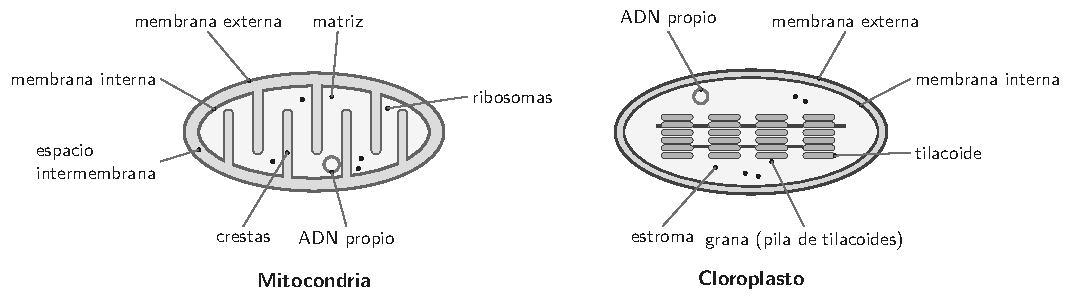
\includegraphics[max width=0.92\linewidth,max height=8.5cm]{bio/cel_mito_cloro}
\end{center}
 
\begin{clave}[{Recuerda}] Mitocondrias y cloroplastos tienen doble membrana, ADN y ribosomas propios. Las células vegetales tienen ambos organelos.\end{clave}
\subsection{La ruta de secreción y cómo se estudia}
\begin{center}
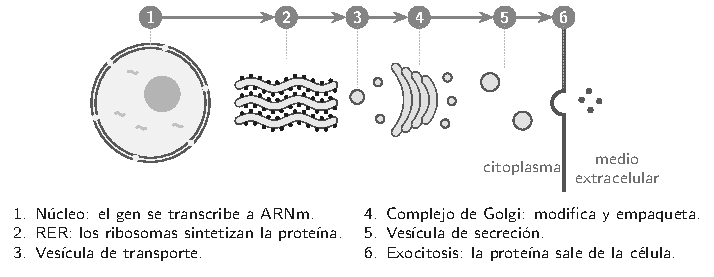
\includegraphics[max width=0.92\linewidth,max height=8.5cm]{bio/cel_secrecion}
\end{center}
  

\textbf{Marcaje radiactivo (pulso y caza).} Se entrega a las células, por pocos minutos, un aminoácido radiactivo (el \textbf{pulso}); luego se cambia por el mismo aminoácido sin marca (la \textbf{caza}). Las proteínas fabricadas durante el pulso quedan marcadas y se puede seguir dónde está la radiactividad a lo largo del tiempo: aparece primero en el \textbf{RER}, luego en el \textbf{Golgi} y al final en las \textbf{vesículas de secreción} y fuera de la célula.

  

\textbf{Organelos inhibidos.} Si un fármaco bloquea un paso, la proteína se \textbf{acumula en el compartimento anterior} al bloqueo y no llega a los siguientes. Por ejemplo, si se bloquea el paso del RER al Golgi, la marca queda en el RER; si se bloquea la salida del Golgi, la marca se acumula en el Golgi y no aparecen vesículas de secreción marcadas.

 
\begin{clave}[{Recuerda}] Para saber qué paso está bloqueado, busca el último compartimento donde la marca se acumula: el bloqueo está justo a la salida de ese compartimento.\end{clave}
\subsection{Lo clave del tema}
\begin{center}\small
\begin{tabularx}{\linewidth}{@{}>{\raggedright\arraybackslash\hsize=0.52\hsize}X>{\raggedright\arraybackslash\hsize=1.29\hsize}X>{\raggedright\arraybackslash\hsize=1.19\hsize}X@{}}
\toprule
\textbf{Organelo} & \textbf{Función principal} & \textbf{Si falla\dots{}} \\
\midrule
Nucléolo & arma subunidades de ribosomas & menos ribosomas \\
RER & sintetiza proteínas de secreción y de membrana & no se forman esas proteínas \\
REL & lípidos, esteroides, detoxificación, Ca\textsuperscript{2+} & se acumulan tóxicos; menos esteroides \\
Golgi & modifica, clasifica y empaqueta & proteínas retenidas, sin secretar \\
Lisosoma & digestión intracelular & material sin digerir acumulado \\
Peroxisoma & oxida ácidos grasos; degrada H\textsubscript{2}O\textsubscript{2} & acumulación de H\textsubscript{2}O\textsubscript{2} \\
Mitocondria & respiración celular: ATP & menos O\textsubscript{2} consumido y menos ATP \\
Citoesqueleto & forma, transporte interno, movimiento & la célula no migra ni mueve vesículas \\
\bottomrule
\end{tabularx}
\end{center}
 
\begin{clave}[{Método PAES}] 1. Subraya el efecto observado (menos ATP, H\textsubscript{2}O\textsubscript{2} acumulado, no se mueve, no secreta). 2. Pregúntate qué organelo produce o controla eso. 3. En experimentos de marcaje, sigue la ruta RER \ensuremath{\rightarrow} Golgi \ensuremath{\rightarrow} vesículas \ensuremath{\rightarrow} membrana y busca dónde se detiene la marca. 4. Distingue el efecto \textbf{directo} (el primero) de las consecuencias posteriores.\end{clave}
\begin{elejemplo}{PAES Invierno 2027, adaptada}
Para estudiar cómo se secretan las enzimas digestivas, se incubaron cortes de páncreas durante 3 minutos con un aminoácido radiactivo (pulso) y luego con el mismo aminoácido sin marca. A distintos tiempos se midió qué porcentaje de la radiactividad de las proteínas estaba en cada compartimento celular:
\begin{center}
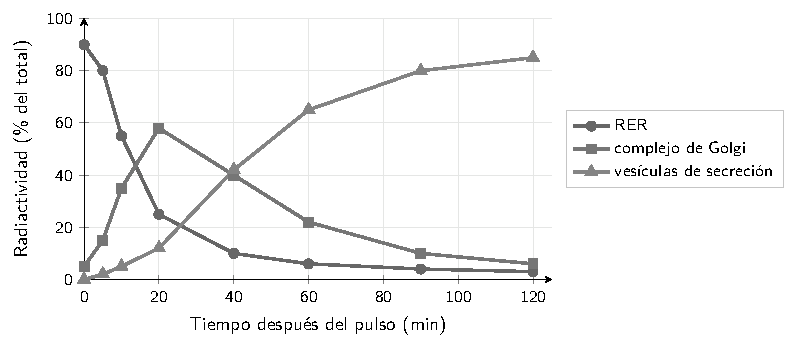
\includegraphics[max width=0.92\linewidth,max height=8.5cm]{bio/cel_pulso}
\end{center}
\altslargas{Las proteínas de secreción se sintetizan en el complejo de Golgi y luego pasan al RER.}{Las proteínas de secreción pasan del RER al complejo de Golgi y luego a las vesículas de secreción.}{Las vesículas de secreción sintetizan proteínas a partir del aminoácido marcado.}{La radiactividad desaparece de la célula a los 20 minutos.}
\solucion{\textbf{Paso 1. ¿Qué nos piden?} La conclusión que se desprende del orden en que la marca pasa por los compartimentos.

\textbf{Paso 2. Busca dónde está la marca al inicio.} Justo después del pulso, cerca del 90 \% de la radiactividad está en el \textbf{RER}: ahí se sintetizaron las proteínas con el aminoácido marcado.

\textbf{Paso 3. Sigue los máximos.} La marca del RER baja mientras sube la del \textbf{Golgi}, que llega a su máximo a los 20 minutos. Luego baja la del Golgi y sube la de las \textbf{vesículas de secreción}, que a los 120 minutos tienen el 85 \%.

\textbf{Respuesta:} las proteínas pasan del RER al complejo de Golgi y luego a las vesículas de secreción.

\textbf{¿Por qué no las otras?} El Golgi alcanza su máximo \textbf{después} que el RER, así que el orden es RER \ensuremath{\rightarrow} Golgi, no al revés. Las vesículas no sintetizan proteínas: reciben la marca al final, cuando ya pasó por el RER y el Golgi. La radiactividad no desaparece: a los 20 minutos está repartida entre RER, Golgi y vesículas, y la suma sigue cerca del 100 \%.

\textbf{\color{cienciaD}Para recordar.} El orden de los máximos de marca revela la ruta: RER \ensuremath{\rightarrow} Golgi \ensuremath{\rightarrow} vesículas de secreción.}{B}
\end{elejemplo}
\motivacion{Cada organelo hace su parte para que la célula funcione. Igual tú: cada tema estudiado suma al resultado final.}

%% =====================================================================
%% bio_especializadas
\section[Estructura y función: células especializadas]{Estructura y función: células especializadas}
\modcomun\ \ {\color{gris}\itshape Cómo la forma y los organelos de una célula se relacionan con su función: el enterocito y la célula secretora pancreática, y cómo deducir la función de una célula a partir de tablas y gráficos con la abundancia de sus organelos.\par}
\subsection{La estructura se ajusta a la función}
Casi todas las células de tu cuerpo tienen el mismo ADN, pero no son iguales: durante el desarrollo, cada tipo celular \textbf{expresa genes distintos} y se \textbf{especializa}. El resultado es que su forma y la cantidad de cada organelo calzan con lo que hace.

 

La idea clave para la PAES: \textbf{una célula tiene en abundancia los organelos que más usa}. Si sabes qué hace cada organelo, puedes deducir la función de una célula que nunca has visto, y al revés.

  
\begin{center}\small
\begin{tabularx}{\linewidth}{@{}>{\raggedright\arraybackslash\hsize=1.07\hsize}X>{\raggedright\arraybackslash\hsize=0.93\hsize}X@{}}
\toprule
\textbf{Si la célula\dots{}} & \textbf{tendrá muchos\dots{}} \\
\midrule
secreta proteínas (enzimas, hormonas proteicas, anticuerpos) & RER, Golgi y vesículas de secreción \\
fabrica hormonas esteroidales o detoxifica & REL \\
gasta mucha energía & mitocondrias \\
digiere lo que fagocita & lisosomas \\
absorbe sustancias & microvellosidades (más superficie) \\
se mueve o mueve líquidos & flagelo o cilios \\
\bottomrule
\end{tabularx}
\end{center}
\subsection{El enterocito: una célula para absorber}
Los \textbf{enterocitos} recubren el interior del intestino delgado y absorben los nutrientes ya digeridos (glucosa, aminoácidos, ácidos grasos) para pasarlos a la sangre.

 
\begin{itemize}
  \item \textbf{Microvellosidades:} miles de pliegues de la membrana en el polo que da a la luz del intestino (borde en cepillo). Multiplican la superficie de absorción; sostenidas por microfilamentos de actina.
  \item \textbf{Muchas mitocondrias:} parte de la absorción es \textbf{transporte activo} y gasta ATP; por ejemplo, la bomba de sodio y potasio mantiene el gradiente que permite absorber glucosa.
  \item \textbf{Uniones estrechas:} sellan el espacio entre células vecinas, así las sustancias pasan \textbf{a través} de las células y no entre ellas.
  \item \textbf{REL y Golgi:} rearman las grasas absorbidas y las empaquetan para enviarlas a la linfa.
\end{itemize}
  
\begin{center}
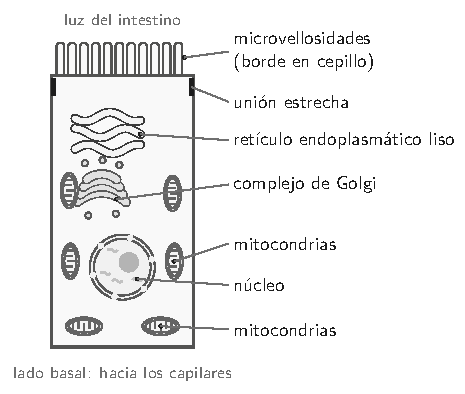
\includegraphics[max width=0.92\linewidth,max height=8.5cm]{bio/cel_enterocito}
\end{center}
\subsection{La célula acinar del páncreas: una célula para secretar}
Las \textbf{células acinares} del páncreas fabrican las enzimas digestivas del jugo pancreático. Tienen forma de pirámide truncada y una organización \textbf{polarizada}, de la base al ápice, que sigue la ruta de secreción:

 
\begin{itemize}
  \item \textbf{Base:} el núcleo y un \textbf{RER muy abundante}, donde se sintetizan las enzimas. El nucléolo es grande: se necesitan muchos ribosomas.
  \item \textbf{Sobre el núcleo:} un \textbf{complejo de Golgi} desarrollado, que modifica y empaqueta las enzimas.
  \item \textbf{Ápice:} muchos \textbf{gránulos de secreción} llenos de enzimas inactivas, que se liberan por exocitosis a la luz del acino.
\end{itemize}
 

Las células beta de los islotes del páncreas también son secretoras de proteínas (insulina) y muestran el mismo patrón: RER y Golgi abundantes.

  
\begin{center}
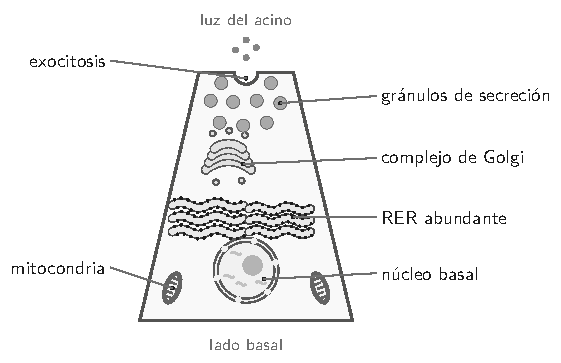
\includegraphics[max width=0.92\linewidth,max height=8.5cm]{bio/cel_acinar}
\end{center}
\subsection{Leer tablas y gráficos de organelos}
Muchas preguntas entregan una tabla o un gráfico con el \textbf{porcentaje del volumen celular} que ocupa cada organelo en varias células, y piden deducir su función. El procedimiento:

 
\begin{itemize}
  \item \textbf{1.} Para cada célula, busca el organelo que \textbf{destaca} respecto de las demás células.
  \item \textbf{2.} Traduce ese organelo a su función (usa la tabla de la primera diapositiva).
  \item \textbf{3.} Une esa función con el tipo de célula que la necesita.
\end{itemize}
 

Algunas parejas que conviene conocer:

 
\begin{itemize}
  \item \textbf{Célula plasmática} (secreta anticuerpos): RER y Golgi.
  \item \textbf{Células de Leydig} del testículo y de la corteza suprarrenal (hormonas esteroidales): REL.
  \item \textbf{Hepatocito:} REL (detoxificación), mitocondrias y peroxisomas.
  \item \textbf{Neutrófilos y macrófagos} (fagocitan): lisosomas.
\end{itemize}
  
\begin{ejemplo}[{Ejemplo resuelto}] En una célula las mitocondrias ocupan el 35 \% del volumen y en otra, el 6 \%. La primera tiene una capacidad mucho mayor de producir ATP: corresponde a una célula con alto gasto de energía sostenido, como las del músculo de vuelo de un ave que migra sin detenerse.\end{ejemplo}
 
\begin{clave}[{Recuerda}] Compara siempre entre células: un 8 \% de mitocondrias puede ser «mucho» o «poco» según con qué lo compares. Y lee bien las unidades del eje.\end{clave}
\subsection{Lo clave del tema}
\begin{center}\small
\begin{tabularx}{\linewidth}{@{}>{\raggedright\arraybackslash\hsize=0.80\hsize}X>{\raggedright\arraybackslash\hsize=0.93\hsize}X>{\raggedright\arraybackslash\hsize=1.28\hsize}X@{}}
\toprule
\textbf{Célula} & \textbf{Función} & \textbf{Estructuras destacadas} \\
\midrule
Enterocito & absorber nutrientes & microvellosidades, mitocondrias, uniones estrechas \\
Célula acinar pancreática & secretar enzimas & RER y Golgi abundantes, gránulos de secreción apicales \\
Célula plasmática & secretar anticuerpos & RER y Golgi abundantes \\
Célula de Leydig & fabricar testosterona & REL abundante \\
Neutrófilo & fagocitar y digerir bacterias & lisosomas abundantes \\
\bottomrule
\end{tabularx}
\end{center}
 
\begin{clave}[{Recuerda}] · Las microvellosidades aumentan la superficie de absorción.\par · Muchas mitocondrias indican un alto gasto de ATP, por ejemplo para el transporte activo o un trabajo sostenido.\par · En una célula secretora, el orden de base a ápice es núcleo y RER \ensuremath{\rightarrow} Golgi \ensuremath{\rightarrow} gránulos.\end{clave}
 
\begin{clave}[{Método PAES}] 1. Identifica el organelo o la estructura que destaca. 2. Recuerda su función. 3. Elige la célula o la función que necesita esa estructura. 4. En experimentos, pregúntate qué pasa si esa estructura falta o se daña: su función disminuye.\end{clave}
\begin{elejemplo}{PAES Invierno 2026, adaptada}
Un grupo de investigadores midió, en tres tipos celulares, qué porcentaje del volumen de la célula ocupan cuatro organelos. Los resultados (datos hipotéticos) se muestran en el gráfico:

¿Qué asociación entre célula y función es más coherente con estos datos?
\begin{center}
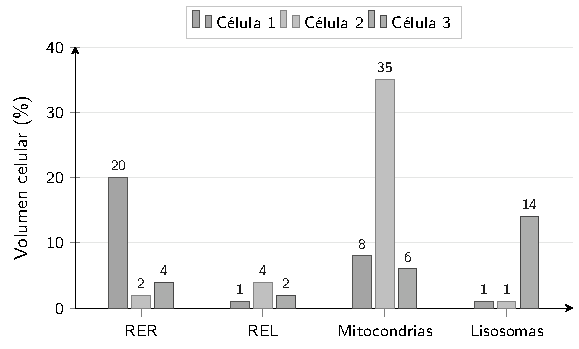
\includegraphics[max width=0.92\linewidth,max height=8.5cm]{bio/cel_vol_1}
\end{center}
\altslargas{Célula 1: secreción de enzimas digestivas.}{Célula 2: síntesis de hormonas esteroidales.}{Célula 3: contracción sostenida con alto gasto de ATP.}{Célula 1: digestión de bacterias fagocitadas.}
\solucion{\textbf{Paso 1. ¿Qué nos piden?} Relacionar el organelo que destaca en cada célula con una función.

\textbf{Paso 2. Busca lo que destaca.} Célula 1: el \textbf{RER} (20 \%, mucho más que en las otras). Célula 2: las \textbf{mitocondrias} (35 \%). Célula 3: los \textbf{lisosomas} (14 \%).

\textbf{Paso 3. Traduce a funciones.} Mucho RER \ensuremath{\rightarrow} síntesis de proteínas para secretar, como las enzimas digestivas. Muchas mitocondrias \ensuremath{\rightarrow} alto gasto de ATP, como en un músculo que se contrae sin pausa. Muchos lisosomas \ensuremath{\rightarrow} digestión intracelular, como en una célula que fagocita bacterias.

\textbf{Respuesta:} célula 1: secreción de enzimas digestivas.

\textbf{¿Por qué no las otras?} La síntesis de hormonas esteroidales necesita mucho REL, y la célula 2 tiene apenas 4 \%. La contracción sostenida corresponde a la célula 2 (mitocondrias), no a la 3. La digestión de bacterias fagocitadas corresponde a la célula 3 (lisosomas), no a la 1.

\textbf{\color{cienciaD}Para recordar.} Organelo que destaca \ensuremath{\rightarrow} función: RER = secretar proteínas; mitocondrias = gastar energía; lisosomas = digerir.}{A}
\end{elejemplo}
\motivacion{Forma y función van de la mano: ya entiendes por qué una neurona no se parece a un glóbulo rojo. ¡Excelente!}

\chapter{Procesos y funciones biológicas}
%% =====================================================================
%% bio_neurona
\section[Organización del sistema nervioso]{Organización del sistema nervioso}
\modcomun\ \ {\color{gris}\itshape Cómo coordina el sistema nervioso las respuestas del cuerpo frente a los estímulos y cómo se organiza: sistema nervioso central y periférico, divisiones somática y autónoma, y acciones opuestas de las divisiones simpática y parasimpática.\par}
\subsection{Cómo se organiza el sistema nervioso}
El sistema nervioso \textbf{coordina e integra} lo que hace el cuerpo frente a los \textbf{estímulos}, tanto externos (luz, sonido, calor) como internos (falta de agua, aumento de CO\textsubscript{2}). Cumple tres funciones en cadena:

 
\begin{itemize}
  \item \textbf{Sensitiva:} los receptores captan el estímulo.
  \item \textbf{Integradora:} el sistema nervioso central procesa la información y elabora una respuesta.
  \item \textbf{Motora:} la respuesta llega a un \textbf{efector}, un músculo o una glándula.
\end{itemize}
 

\textbf{Sistema nervioso central (SNC):} encéfalo (cerebro, cerebelo y tronco encefálico) y médula espinal. Está protegido por el cráneo, la columna vertebral, las meninges y el líquido cefalorraquídeo.

 

\textbf{Sistema nervioso periférico (SNP):} los nervios (12 pares craneales y 31 pares raquídeos) y los ganglios. Conecta el SNC con el resto del cuerpo.

  
\begin{clave}[{Las divisiones del SNP}] · \textbf{Somático:} controla los músculos esqueléticos; es voluntario (levantar la mano, caminar).\par · \textbf{Autónomo:} controla el corazón, el músculo liso y las glándulas; es involuntario.\par · \textbf{Simpático:} prepara para la acción, «lucha o huida»: aumenta la frecuencia cardíaca, dilata las pupilas y los bronquios, frena la digestión.\par · \textbf{Parasimpático:} «reposo y digestión»: baja la frecuencia cardíaca, contrae las pupilas, estimula la salivación y los movimientos del tubo digestivo.\end{clave}
  
\begin{center}
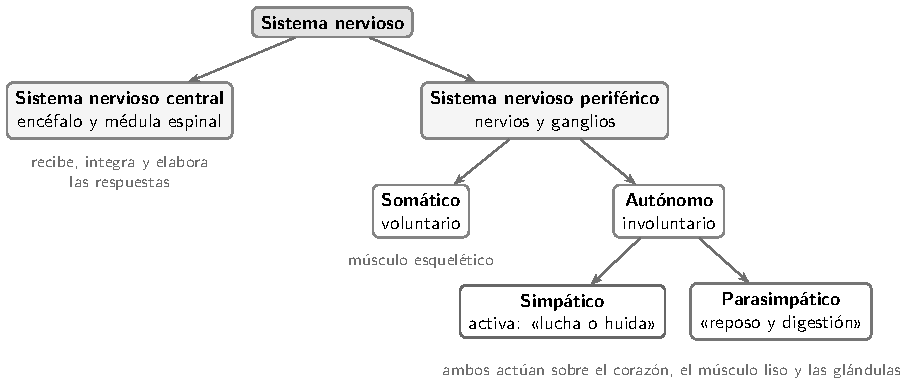
\includegraphics[max width=0.92\linewidth,max height=8.5cm]{bio/ner_organizacion}
\end{center}
\subsection{Lo clave del tema}
\begin{center}\small
\begin{tabularx}{\linewidth}{@{}>{\raggedright\arraybackslash\hsize=0.74\hsize}X>{\raggedright\arraybackslash\hsize=1.13\hsize}X>{\raggedright\arraybackslash\hsize=1.13\hsize}X@{}}
\toprule
\textbf{Parte} & \textbf{Qué incluye} & \textbf{Qué hace} \\
\midrule
SNC & encéfalo (cerebro, cerebelo, tronco encefálico) y médula espinal & integra la información y elabora respuestas \\
SNP somático & nervios hacia y desde la piel y los músculos esqueléticos & sensibilidad y movimiento voluntario \\
SNP autónomo simpático & nervios hacia el corazón, el músculo liso y las glándulas & «lucha o huida»: sube la frecuencia cardíaca, dilata pupilas y bronquios, frena la digestión \\
SNP autónomo parasimpático & nervios hacia los mismos órganos & «reposo y digestión»: baja la frecuencia cardíaca, contrae las pupilas, estimula la digestión \\
\bottomrule
\end{tabularx}
\end{center}
 
\begin{clave}[{Recuerda}] · Funciones en cadena: sensitiva (receptor) \ensuremath{\rightarrow} integradora (SNC) \ensuremath{\rightarrow} motora (efector: músculo o glándula).\par · SNC = encéfalo y médula espinal; SNP = nervios y ganglios.\par · El somático es voluntario; el autónomo es involuntario.\par · El simpático activa («lucha o huida»); el parasimpático favorece el reposo y la digestión.\end{clave}
 
\begin{clave}[{Método PAES}] 1. Pregúntate si la respuesta es voluntaria (somático) o involuntaria (autónomo). 2. Si es involuntaria, decide si prepara para la acción (simpático) o para el reposo y la digestión (parasimpático). 3. Para ubicar una estructura, recuerda que el SNC es solo encéfalo y médula espinal: todo nervio o ganglio es SNP.\end{clave}
\begin{elejemplo}{Estilo PAES}
Una persona camina de noche por una calle oscura y escucha un ruido fuerte detrás de ella. En pocos segundos su corazón late más rápido, sus pupilas se dilatan y su respiración se acelera. Estas respuestas son involuntarias.

¿Qué parte del sistema nervioso produce principalmente estas respuestas?
\altslargas{La división simpática del sistema nervioso autónomo.}{La división parasimpática del sistema nervioso autónomo.}{El sistema nervioso somático.}{El cerebelo, que coordina el equilibrio.}
\solucion{\textbf{Paso 1. ¿Qué nos piden?} La división que controla respuestas \textbf{involuntarias} que preparan al cuerpo frente a un peligro.

\textbf{Paso 2. Involuntario \ensuremath{\rightarrow} autónomo.} El corazón, el músculo de la pupila y los bronquios no se controlan a voluntad: los regula el sistema nervioso autónomo.

\textbf{Paso 3. ¿Cuál de sus divisiones?} Aumentar la frecuencia cardíaca, dilatar las pupilas y acelerar la respiración son respuestas de «lucha o huida»: las produce la división \textbf{simpática}.

\textbf{Respuesta:} la división simpática del sistema nervioso autónomo.

\textbf{¿Por qué no las otras?} La división parasimpática hace lo contrario: baja la frecuencia cardíaca y contrae las pupilas. El sistema somático controla los músculos esqueléticos de forma voluntaria. El cerebelo coordina el equilibrio y los movimientos, no el ritmo cardíaco ni las pupilas.

\textbf{\color{cienciaD}Para recordar.} Respuestas involuntarias de alerta («lucha o huida») = simpático.}{A}
\end{elejemplo}
\motivacion{Tu sistema nervioso acaba de aprender cómo funciona el sistema nervioso. ¡Eso sí que es pensar!}

%% =====================================================================
%% bio_sinapsis
\section[Arco reflejo, drogas y cuidado del sistema nervioso]{Arco reflejo, drogas y cuidado del sistema nervioso}
\modcomun\ \ {\color{gris}\itshape Cómo funciona el arco reflejo simple, qué efectos tienen la cafeína, el alcohol y las drogas de abuso sobre el sistema nervioso y qué cuidados lo protegen: dormir lo suficiente y prevenir traumatismos.\par}
\subsection{El arco reflejo}
Un \textbf{reflejo} es una respuesta \textbf{rápida, involuntaria y predecible} frente a un estímulo: retirar la mano de una olla caliente, el reflejo rotuliano, el parpadeo. El camino que sigue el impulso es el \textbf{arco reflejo}, con cinco componentes:

 
\begin{itemize}
  \item \textbf{Receptor:} capta el estímulo (en la piel, un receptor de dolor o de calor).
  \item \textbf{Vía aferente:} una neurona sensitiva lleva el impulso hacia el SNC. Entra a la médula por la raíz dorsal; su soma está en un ganglio.
  \item \textbf{Centro elaborador:} la médula espinal (o el tronco encefálico). Ahí la información pasa, a menudo a través de una interneurona, a una neurona motora.
  \item \textbf{Vía eferente:} una neurona motora lleva la orden hacia el efector.
  \item \textbf{Efector:} el músculo que se contrae o la glándula que secreta.
\end{itemize}
  
\begin{clave}[{¿Por qué es tan rápido?}] La respuesta se elabora en la médula, pasando por muy pocas neuronas, sin esperar al encéfalo. Al mismo tiempo, la información sube por la médula hasta el encéfalo: por eso sientes el dolor un instante \textbf{después} de haber retirado la mano.\end{clave}
 
\begin{clave}[{Recuerda}] El reflejo rotuliano es el arco más simple: la neurona sensitiva se conecta directamente con la neurona motora, sin interneurona.\end{clave}
  
\begin{center}
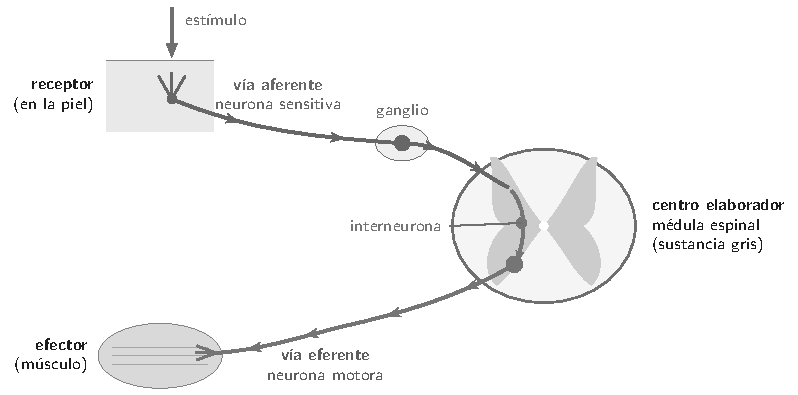
\includegraphics[max width=0.92\linewidth,max height=8.5cm]{bio/ner_arco}
\end{center}
\subsection{El café y la cafeína}
Mientras estamos despiertos, la actividad del encéfalo acumula \textbf{adenosina}. La adenosina se une a sus receptores en las neuronas y \textbf{disminuye} su actividad: así aparece la sensación de cansancio y sueño.

 

La \textbf{cafeína} (del café, el té, el mate, las bebidas cola y las bebidas energéticas) tiene una forma parecida a la adenosina. Se une a los receptores de adenosina \textbf{sin activarlos} y los bloquea. Resultado: la adenosina no puede actuar, y la persona se siente más alerta y con menos sueño.

 

La cafeína tarda unas 5 horas en reducirse a la mitad en la sangre. Por eso un café en la tarde puede retrasar el sueño en la noche.

  
\begin{clave}[{Efectos del consumo alto}] Insomnio, nerviosismo, ansiedad, taquicardia y molestias digestivas. Con el consumo diario aparece \textbf{tolerancia} (se necesita más para el mismo efecto), y al suspenderlo puede haber dolor de cabeza y cansancio por un par de días.\end{clave}
  
\begin{center}
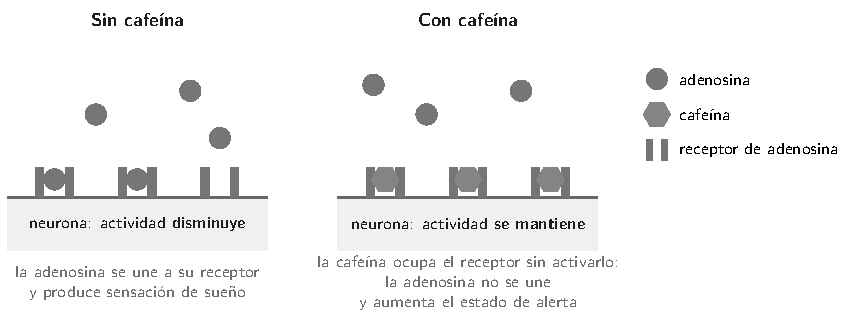
\includegraphics[max width=0.92\linewidth,max height=8.5cm]{bio/ner_cafeina}
\end{center}
\subsection{Alcohol y drogas de abuso}
Muchas sustancias alteran el funcionamiento del sistema nervioso y, con él, la conducta. Algunas lo \textbf{deprimen}: hacen más lentas sus respuestas. Otras lo \textbf{estimulan}: aumentan la alerta y la actividad.

 
\begin{center}\small
\begin{tabularx}{\linewidth}{@{}>{\raggedright\arraybackslash\hsize=0.63\hsize}X>{\raggedright\arraybackslash\hsize=0.79\hsize}X>{\raggedright\arraybackslash\hsize=1.58\hsize}X@{}}
\toprule
\textbf{Sustancia} & \textbf{Tipo} & \textbf{Efectos} \\
\midrule
Alcohol (etanol) & depresor del SNC & reflejos más lentos, falta de coordinación, peor juicio; en dosis altas, pérdida de conciencia y depresión respiratoria \\
Nicotina & estimulante & aumenta la alerta y la frecuencia cardíaca; muy adictiva \\
Cocaína & estimulante & euforia, taquicardia, hipertensión; alto riesgo de adicción \\
Anfetaminas & estimulantes & alerta, insomnio, taquicardia \\
Marihuana (THC) & altera la percepción & afecta la memoria, la atención y la coordinación \\
\bottomrule
\end{tabularx}
\end{center}
 
\begin{clave}[{Tolerancia y dependencia}] Las drogas de abuso activan el \textbf{circuito de recompensa} del encéfalo, el que produce la sensación de placer. Con el consumo repetido, el encéfalo se adapta: aparece la \textbf{tolerancia} (se necesita más droga para el mismo efecto), y al dejar la sustancia, el \textbf{síndrome de abstinencia}. Este cambio en el circuito de recompensa es la base de la adicción.\end{clave}
 
\begin{clave}[{Alcohol y conducción en Chile}] La ley considera «bajo la influencia del alcohol» a quien conduce con más de 0,3 g de alcohol por litro de sangre, y «en estado de ebriedad» desde 0,8 g/L. El alcohol alarga el tiempo de reacción incluso en dosis bajas.\end{clave}
\subsection{Cuidar el sistema nervioso}
\textbf{Dormir lo suficiente.} Durante el sueño el encéfalo consolida lo aprendido en el día (la memoria) y se recupera. Dormir poco empeora la atención, la memoria, el ánimo y el tiempo de reacción.

 
\begin{center}\small
\begin{tabular}{@{}ll@{}}
\toprule
\textbf{Edad} & \textbf{Horas de sueño recomendadas} \\
\midrule
6 a 12 años & 9 a 12 h \\
13 a 18 años & 8 a 10 h \\
Adultos & 7 a 9 h \\
\bottomrule
\end{tabular}
\end{center}
 

Ayudan a dormir bien: horarios regulares, evitar pantallas antes de acostarse y no tomar cafeína en la tarde.

  

\textbf{Prevenir traumatismos.} Las neuronas del SNC casi no se reemplazan cuando mueren: un daño en el encéfalo o en la médula espinal suele dejar secuelas permanentes.

 
\begin{itemize}
  \item \textbf{Traumatismo encéfalo craneano (TEC):} golpe en la cabeza en accidentes de tránsito, caídas o deportes. Se previene con \textbf{casco} (bicicleta, scooter, moto, esquí) y \textbf{cinturón de seguridad}, y con sillas para niños en el auto.
  \item \textbf{Lesión de la médula espinal:} se pierde la sensibilidad y el movimiento voluntario de las zonas del cuerpo que dependen de la médula bajo la lesión. Una causa frecuente en verano es lanzarse de cabeza en aguas poco profundas.
\end{itemize}
\subsection{Lo clave del tema}
\begin{center}\small
\begin{tabularx}{\linewidth}{@{}>{\raggedright\arraybackslash\hsize=0.67\hsize}X>{\raggedright\arraybackslash\hsize=1.33\hsize}X@{}}
\toprule
\textbf{Tema} & \textbf{Lo esencial} \\
\midrule
Arco reflejo & respuesta rápida e involuntaria que se elabora en la médula; si se corta una parte, lo que está antes del corte sigue funcionando \\
Cafeína & bloquea los receptores de adenosina: menos sueño; en exceso, insomnio, ansiedad y taquicardia \\
Alcohol & depresor del SNC: alarga el tiempo de reacción incluso en dosis bajas \\
Drogas de abuso & activan el circuito de recompensa: tolerancia, abstinencia y adicción \\
Sueño y traumatismos & el sueño consolida la memoria; las neuronas del SNC casi no se reemplazan \\
\bottomrule
\end{tabularx}
\end{center}
 
\begin{clave}[{Recuerda}] · Arco reflejo: receptor \ensuremath{\rightarrow} vía aferente \ensuremath{\rightarrow} centro elaborador (médula) \ensuremath{\rightarrow} vía eferente \ensuremath{\rightarrow} efector.\par · El reflejo es involuntario y rápido porque se elabora en la médula, sin esperar al encéfalo.\par · La cafeína bloquea los receptores de adenosina; el alcohol es un depresor del SNC.\par · Adolescentes: 8 a 10 horas de sueño. Casco y cinturón previenen traumatismos.\end{clave}
 
\begin{clave}[{Método PAES}] 1. En un arco reflejo, sigue el camino del impulso y fíjate qué parte quedó cortada: lo que está antes del corte sigue funcionando. 2. En un gráfico sobre una sustancia o sobre el sueño, describe la tendencia sin ir más allá de los datos. 3. En un experimento, busca el grupo control y la variable que se mide.\end{clave}
\begin{elejemplo}{Estilo PAES}
El esquema representa un arco reflejo. Los números indican sus componentes.

¿Qué números corresponden al centro elaborador y a la vía eferente, respectivamente?
\begin{center}
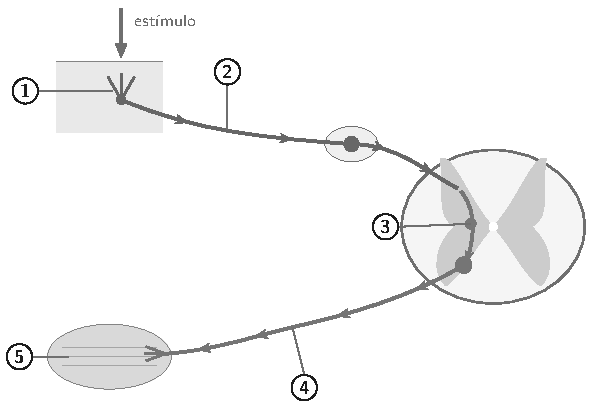
\includegraphics[max width=0.92\linewidth,max height=8.5cm]{bio/ner_arco_num}
\end{center}
\alts{2 y 4}{3 y 2}{3 y 4}{5 y 4}
\solucion{\textbf{Paso 1. ¿Qué nos piden?} El centro elaborador y la vía eferente.

\textbf{Paso 2. Sigue el camino del impulso.} 1: receptor en la piel. 2: neurona sensitiva, que lleva el impulso hacia la médula (vía aferente). 3: interneurona en la médula espinal (centro elaborador). 4: neurona motora, que lleva la orden desde la médula (vía eferente). 5: músculo (efector).

\textbf{Respuesta:} 3 y 4.

\textbf{¿Por qué no las otras?} El 2 es la vía aferente: lleva el impulso \textbf{hacia} el centro, no desde él. El 5 es el efector, el músculo que responde, no el centro elaborador.

\textbf{\color{cienciaD}Para recordar.} Aferente llega al centro; eferente sale del centro hacia el efector.}{C}
\end{elejemplo}
\motivacion{Cuidar tu sistema nervioso también es dormir bien y descansar. Estudia con constancia, no toda la noche antes.}

%% =====================================================================
%% bio_reproduccion
\section[Sistemas reproductores, gametos y fecundación]{Sistemas reproductores, gametos y fecundación}
\modcomun\ \ {\color{gris}\itshape Estructura y función de los sistemas reproductores femenino y masculino, cómo son el ovocito y el espermatozoide, dónde y cómo ocurre la fecundación, el camino del embrión hasta la implantación y las dimensiones de la sexualidad humana.\par}
\subsection{Sistema reproductor femenino}
El sistema reproductor femenino produce los \textbf{ovocitos} y las \textbf{hormonas sexuales}, recibe a los espermatozoides y alberga al embrión durante la gestación.

 
\begin{itemize}
  \item \textbf{Ovarios:} dos glándulas en la cavidad pelviana. Contienen los folículos, donde maduran los ovocitos, y producen \textbf{estrógeno} y \textbf{progesterona}.
  \item \textbf{Trompas uterinas (oviductos):} conductos que van de cada ovario al útero. Sus \textbf{fimbrias} captan el ovocito liberado. En su tercio externo (la ampolla) ocurre la \textbf{fecundación}.
  \item \textbf{Útero:} órgano hueco y muscular. Su pared tiene una capa muscular, el \textbf{miometrio}, que se contrae en el parto, y una capa interna, el \textbf{endometrio}, donde se implanta el embrión y que se desprende en cada menstruación.
  \item \textbf{Cuello uterino:} comunica el útero con la vagina. Produce el \textbf{moco cervical}, que cambia durante el ciclo.
  \item \textbf{Vagina:} conducto que recibe al pene en la relación sexual, por donde sale la menstruación y que forma parte del canal del parto. La \textbf{vulva} son los genitales externos.
\end{itemize}
  
\begin{center}
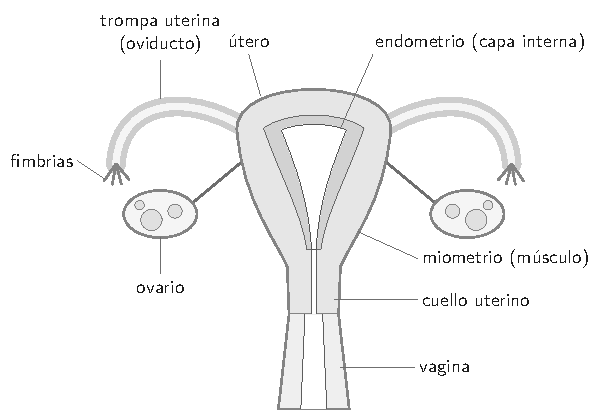
\includegraphics[max width=0.92\linewidth,max height=8.5cm]{bio/rep_femenino}
\end{center}
\subsection{Sistema reproductor masculino}
El sistema reproductor masculino produce los \textbf{espermatozoides} y la hormona \textbf{testosterona}, y los deposita en el sistema femenino.

 
\begin{itemize}
  \item \textbf{Testículos:} en los \textbf{túbulos seminíferos} se forman los espermatozoides (espermatogénesis), de manera continua desde la pubertad. Las \textbf{células de Leydig} producen testosterona.
  \item \textbf{Escroto:} bolsa de piel que aloja los testículos fuera del abdomen, a una temperatura unos 2 a 3 °C menor que la del cuerpo, necesaria para formar espermatozoides.
  \item \textbf{Epidídimo:} tubo enrollado sobre cada testículo. Allí los espermatozoides \textbf{maduran}, adquieren la capacidad de moverse y se almacenan.
  \item \textbf{Conductos deferentes:} llevan los espermatozoides desde el epidídimo hasta la uretra. Son los que se cortan en la vasectomía.
  \item \textbf{Glándulas anexas:} las \textbf{vesículas seminales} aportan un líquido con fructosa (energía); la \textbf{próstata}, un líquido que protege a los espermatozoides de la acidez vaginal; las \textbf{glándulas bulbouretrales}, un líquido que lubrica la uretra. Estos líquidos más los espermatozoides forman el \textbf{semen}.
  \item \textbf{Uretra y pene:} la uretra conduce el semen y también la orina, aunque nunca al mismo tiempo.
\end{itemize}
  
\begin{center}
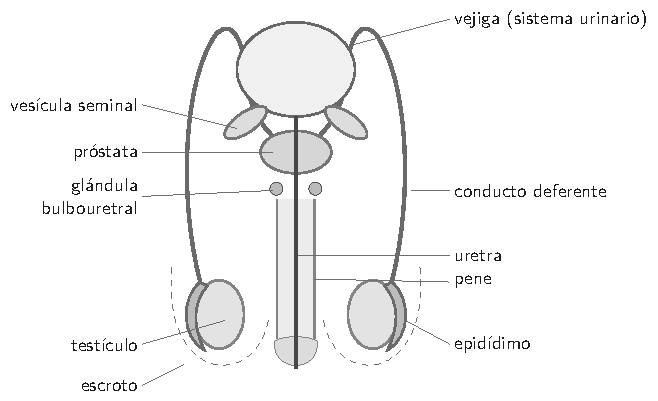
\includegraphics[max width=0.92\linewidth,max height=8.5cm]{bio/rep_masculino}
\end{center}
\subsection{Los gametos: ovocito y espermatozoide}
\begin{center}
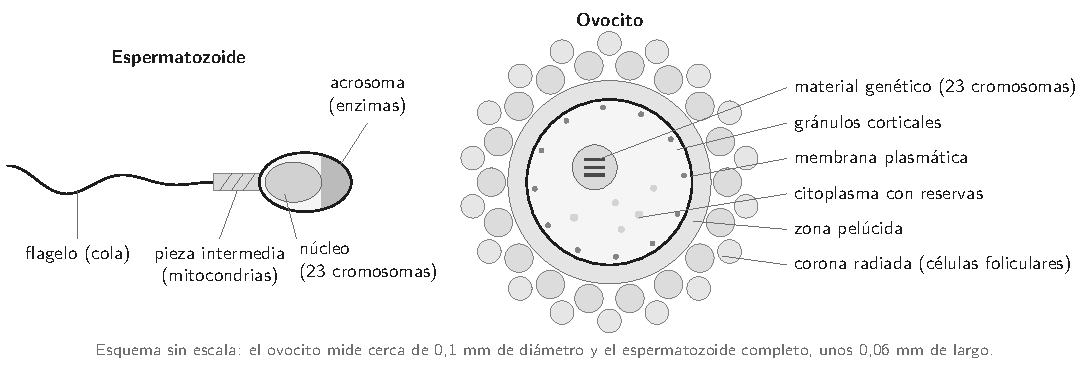
\includegraphics[max width=0.92\linewidth,max height=8.5cm]{bio/rep_gametos}
\end{center}
 
\begin{center}\small
\begin{tabularx}{\linewidth}{@{}>{\raggedright\arraybackslash\hsize=0.60\hsize}X>{\raggedright\arraybackslash\hsize=1.20\hsize}X>{\raggedright\arraybackslash\hsize=1.20\hsize}X@{}}
\toprule
 & \textbf{Espermatozoide} & \textbf{Ovocito} \\
\midrule
Dónde se forma & túbulos seminíferos del testículo & folículos del ovario \\
Cantidad & decenas o cientos de millones en cada eyaculación; se forman de manera continua desde la pubertad & en general uno por ciclo; su formación comienza antes del nacimiento \\
Tamaño y forma & muy pequeño (unos 0,06 mm), con cabeza, pieza intermedia y flagelo & una de las células más grandes del cuerpo (cerca de 0,1 mm), esférico \\
Movilidad & se mueve con su flagelo, gracias al ATP de las mitocondrias de la pieza intermedia & no se mueve por sí mismo; lo desplazan los cilios y las contracciones de la trompa \\
Qué aporta al cigoto & 23 cromosomas, entre ellos un X o un Y, que define el sexo cromosómico & 23 cromosomas (siempre un X), casi todo el citoplasma, las reservas y las mitocondrias \\
\bottomrule
\end{tabularx}
\end{center}
 
\begin{clave}[{Recuerda}] El \textbf{acrosoma} es una vesícula en la punta de la cabeza del espermatozoide. Contiene \textbf{enzimas} que digieren las cubiertas del ovocito (corona radiada y zona pelúcida). El ovocito que se libera en la ovulación está detenido en la segunda división de la meiosis y la termina solo si es fecundado.\end{clave}
\subsection{La fecundación}
La \textbf{fecundación} es la unión del espermatozoide con el ovocito. Ocurre normalmente en el \textbf{tercio externo de la trompa uterina}, poco después de la ovulación.

 

Tras la eyaculación, los espermatozoides recorren vagina, cuello uterino, útero y trompa. En el camino se \textbf{capacitan}: cambia su membrana y quedan listos para fecundar. Solo unos pocos cientos llegan cerca del ovocito.

 

\textbf{Etapas:}

 
\begin{enumerate}
  \item El espermatozoide atraviesa la \textbf{corona radiada}.
  \item Se une a la \textbf{zona pelúcida} y ocurre la \textbf{reacción acrosómica}: el acrosoma libera sus enzimas, que abren un camino a través de la zona pelúcida.
  \item Las \textbf{membranas} de ambos gametos se fusionan y el núcleo del espermatozoide entra al ovocito.
  \item \textbf{Reacción cortical:} los gránulos corticales liberan su contenido y la zona pelúcida cambia, de modo que no entran más espermatozoides (se evita la \textbf{polispermia}).
\end{enumerate}
 

El ovocito termina su meiosis, los dos núcleos (pronúcleos) se unen y se forma el \textbf{cigoto}, con 46 cromosomas: 23 de cada progenitor.

  
\begin{center}
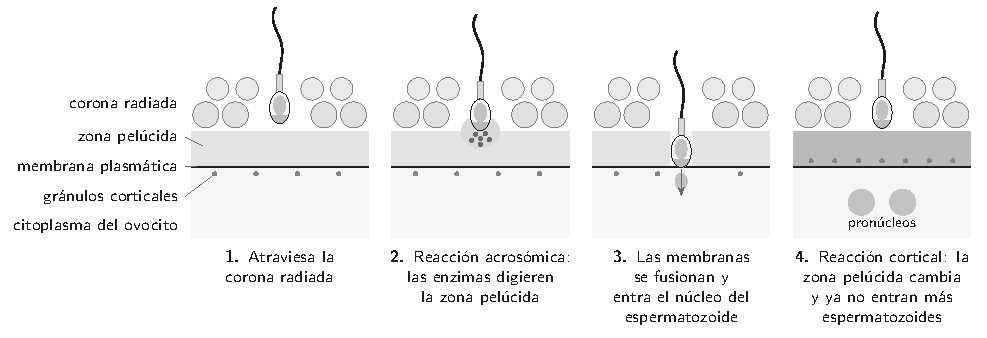
\includegraphics[max width=0.92\linewidth,max height=8.5cm]{bio/rep_fecundacion}
\end{center}
\subsection{Del cigoto a la implantación}
\begin{center}
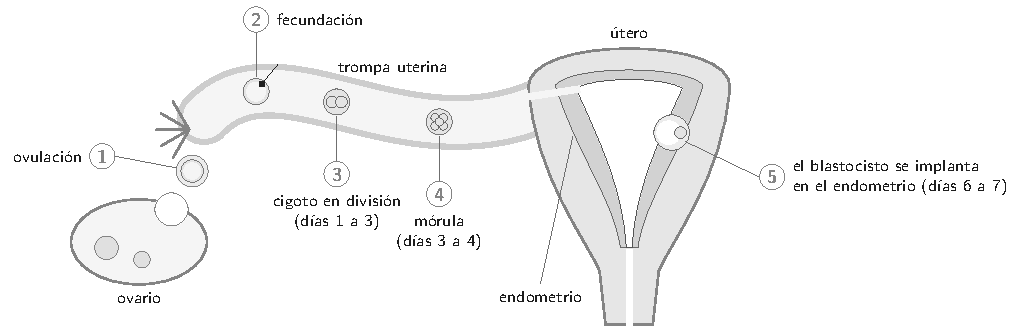
\includegraphics[max width=0.92\linewidth,max height=8.5cm]{bio/rep_trayecto}
\end{center}
  

Mientras viaja por la trompa hacia el útero, el cigoto se divide por mitosis (\textbf{segmentación}): 2, 4, 8 células\dots{} Hacia el día 3 o 4 es una esfera maciza de células, la \textbf{mórula}. Al llegar al útero se transforma en \textbf{blastocisto}, una esfera hueca.

 

Entre los días 6 y 7 después de la fecundación, el blastocisto se \textbf{implanta} (anida) en el \textbf{endometrio}. Sus células externas formarán parte de la \textbf{placenta} y empiezan a producir la hormona \textbf{hCG}, que es la que detectan las pruebas de embarazo.

  
\begin{clave}[{Recuerda}] · Fecundación: en la trompa uterina.\par · Implantación: en el endometrio del útero, unos 6 a 7 días después.\par · Si el embrión se implanta fuera del útero, por ejemplo en la trompa, se habla de embarazo \textbf{ectópico}, una urgencia médica.\par · La hCG se produce después de la implantación; por eso una prueba de embarazo hecha demasiado pronto puede salir negativa.\end{clave}
\subsection{Sexualidad humana}
La sexualidad es parte de la vida de todas las personas y va mucho más allá de la reproducción. Se suele describir con tres dimensiones que se relacionan entre sí:

 
\begin{itemize}
  \item \textbf{Biológica:} anatomía, hormonas, cambios de la pubertad, reproducción y salud sexual.
  \item \textbf{Psicológica y afectiva:} emociones, autoestima, identidad, vínculos, forma de vivir el afecto y la intimidad.
  \item \textbf{Social:} normas, cultura, valores, roles y la influencia de la familia, los pares y los medios.
\end{itemize}
 

Una sexualidad sana contribuye al \textbf{bienestar integral} de la persona y de sus relaciones.

  
\begin{clave}[{Claves para relaciones sanas}] · \textbf{Consentimiento:} libre, informado y entusiasta; se puede retirar en cualquier momento y se pide cada vez.\par · \textbf{Respeto:} a los tiempos, decisiones, límites y diversidad de cada persona.\par · \textbf{Cuidado:} de la propia salud y de la del otro (preservativo, exámenes de ITS, controles de salud).\par · \textbf{Responsabilidad:} tomar decisiones informadas y hacerse cargo de sus consecuencias.\par · \textbf{Comunicación:} conversar con confianza sobre lo que se siente, se quiere y no se quiere.\end{clave}
\subsection{Lo clave del tema}
\begin{center}\small
\begin{tabularx}{\linewidth}{@{}>{\raggedright\arraybackslash\hsize=0.64\hsize}X>{\raggedright\arraybackslash\hsize=1.36\hsize}X@{}}
\toprule
\textbf{Estructura} & \textbf{Función principal} \\
\midrule
Ovario & madura los ovocitos; produce estrógeno y progesterona \\
Trompa uterina & capta el ovocito; lugar de la fecundación; lleva el embrión al útero \\
Endometrio & lugar de implantación; se desprende en la menstruación \\
Testículo & forma espermatozoides (túbulos seminíferos) y testosterona (células de Leydig) \\
Epidídimo & maduración y almacenamiento; los espermatozoides adquieren movilidad \\
Conducto deferente & transporta espermatozoides hacia la uretra \\
Acrosoma & enzimas que digieren la corona radiada y la zona pelúcida \\
Pieza intermedia & mitocondrias que producen el ATP para el flagelo \\
Gránulos corticales & cambian la zona pelúcida y bloquean la polispermia \\
\bottomrule
\end{tabularx}
\end{center}
 
\begin{clave}[{Recuerda}] · Cada gameto tiene 23 cromosomas; el cigoto, 46.\par · El espermatozoide define el sexo cromosómico (lleva X o Y); el ovocito siempre lleva X.\par · El ovocito aporta casi todo el citoplasma y las mitocondrias del cigoto.\par · La fecundación ocurre en la trompa y la implantación, en el endometrio.\end{clave}
 
\begin{clave}[{Método PAES}] 1. Ubica la estructura o el proceso del que habla el enunciado (esquema numerado, gameto, etapa). 2. Recuerda su función. 3. Predice qué pasa si esa estructura falla: ¿qué paso de la reproducción se interrumpe y cuáles siguen igual? 4. En experimentos, compara cada grupo con el control y concluye solo lo que muestran los datos.\end{clave}
\begin{elejemplo}{PAES Regular 2026, adaptada}
Un espermiograma muestra que los espermatozoides de un paciente tienen forma normal y están en cantidad adecuada, pero casi no se desplazan. Al microscopio electrónico se observa que sus mitocondrias están alteradas. El siguiente esquema muestra las partes de un espermatozoide:

¿Qué estructura del esquema está alterada y qué función se ve afectada?
\begin{center}
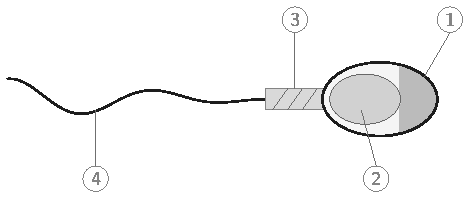
\includegraphics[max width=0.92\linewidth,max height=8.5cm]{bio/rep_esperm_num}
\end{center}
\altslargas{La estructura 1, que libera enzimas para atravesar las cubiertas del ovocito.}{La estructura 2, que aporta la información genética al cigoto.}{La estructura 3, que produce el ATP que mueve el flagelo.}{La estructura 4, que almacena las reservas de energía del espermatozoide.}
\solucion{\textbf{Paso 1. ¿Qué nos piden?} Relacionar un dato (mitocondrias alteradas y poco movimiento) con una parte del espermatozoide y su función.

\textbf{Paso 2. Identifica las partes.} 1 es el acrosoma, 2 el núcleo, 3 la pieza intermedia y 4 el flagelo.

\textbf{Paso 3. ¿Dónde están las mitocondrias?} En la \textbf{pieza intermedia}, enrolladas alrededor del inicio del flagelo. Producen el \textbf{ATP} que el flagelo usa para moverse. Si fallan, el flagelo existe pero no tiene energía: el espermatozoide casi no se desplaza.

\textbf{Respuesta:} la estructura 3, que produce el ATP que mueve el flagelo.

\textbf{¿Por qué no las otras?} El acrosoma (1) participa en la fecundación, no en el movimiento, y no tiene mitocondrias. El núcleo (2) lleva los cromosomas; su alteración no explica la falta de movimiento. El flagelo (4) es el que se mueve, pero no almacena reservas ni tiene mitocondrias: recibe la energía desde la pieza intermedia.

\textbf{\color{cienciaD}Para recordar.} Las mitocondrias de la pieza intermedia producen el ATP que mueve el flagelo.}{C}
\end{elejemplo}
\motivacion{Gametos, fecundación y sistemas reproductores: un tema largo y ya es tuyo. Te ganaste un descanso con ronroneo.}

%% =====================================================================
%% bio_ciclo
\section[Ciclo ovárico y ciclo uterino]{Ciclo ovárico y ciclo uterino}
\modcomun\ \ {\color{gris}\itshape Las fases del ciclo ovárico (folicular, ovulación y lútea) y del ciclo uterino (menstrual, proliferativa y secretora), las hormonas FSH, LH, estrógeno y progesterona, su regulación por el eje hipotálamo-hipófisis-ovario, la lectura de gráficos de 28 días y qué cambia si hay fecundación.\par}
\subsection{Dos ciclos que van juntos}
Desde la pubertad hasta la menopausia, el sistema reproductor femenino repite un ciclo que prepara, cada mes, un ovocito para ser fecundado y un endometrio para recibir al embrión. En realidad son \textbf{dos ciclos coordinados por hormonas}:

 
\begin{itemize}
  \item \textbf{Ciclo ovárico:} ocurre en el \textbf{ovario}. Madura un folículo, se libera un ovocito y se forma el cuerpo lúteo.
  \item \textbf{Ciclo uterino (o menstrual):} ocurre en el \textbf{endometrio}. Se desprende, crece y se prepara para la implantación.
\end{itemize}
 

Por convención, el \textbf{día 1} es el primer día de la menstruación. Un ciclo dura en promedio \textbf{28 días}, aunque es normal que dure entre unos 21 y 35 días y que varíe un poco de un mes a otro.

  
\begin{clave}[{Las cuatro hormonas del ciclo}] · \textbf{FSH} (hormona folículo estimulante), de la hipófisis: hace crecer los folículos.\par · \textbf{LH} (hormona luteinizante), de la hipófisis: su pico provoca la ovulación y forma el cuerpo lúteo.\par · \textbf{Estrógeno}, del folículo: engrosa el endometrio.\par · \textbf{Progesterona}, del cuerpo lúteo: prepara y mantiene el endometrio.\end{clave}
\subsection{El ciclo ovárico}
\begin{center}
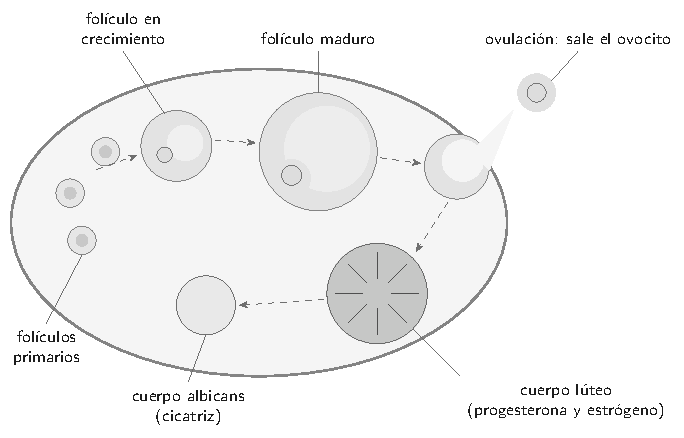
\includegraphics[max width=0.92\linewidth,max height=8.5cm]{bio/rep_ovario}
\end{center}
  

\textbf{Fase folicular} (días 1 a 13, aproximadamente). La \textbf{FSH} estimula el crecimiento de varios folículos; uno se vuelve dominante y llega a \textbf{folículo maduro}. Sus células producen cada vez más \textbf{estrógeno}.

 

\textbf{Ovulación} (cerca del día 14). Un \textbf{pico de LH} hace que el folículo maduro se rompa y libere el ovocito, que es captado por la trompa.

  

\textbf{Fase lútea} (días 15 a 28). Por acción de la LH, el folículo roto se transforma en \textbf{cuerpo lúteo}, que secreta \textbf{progesterona} y algo de estrógeno. Si no hay fecundación, el cuerpo lúteo dura unos 10 a 14 días y degenera en una cicatriz (cuerpo albicans).

 
\begin{clave}[{Recuerda}] La fase lútea dura casi siempre unos 14 días. Lo que cambia entre ciclos largos y cortos es la fase folicular. Por eso la ovulación ocurre unos \textbf{14 días antes} de la siguiente menstruación: en un ciclo de 32 días, cerca del día 18.\end{clave}
\subsection{El ciclo uterino}
\begin{itemize}
  \item \textbf{Fase menstrual} (días 1 a 5, aproximadamente): al caer la progesterona y el estrógeno, la capa superficial del endometrio se desprende y sale con sangre: es la \textbf{menstruación}.
  \item \textbf{Fase proliferativa} (días 6 a 14): el \textbf{estrógeno} del folículo hace que el endometrio se regenere y se engrose.
  \item \textbf{Fase secretora} (días 15 a 28): la \textbf{progesterona} del cuerpo lúteo hace que el endometrio se llene de glándulas y vasos sanguíneos, quede más grueso y secrete nutrientes. Está listo para recibir un embrión.
\end{itemize}
 
\begin{center}\small
\begin{tabularx}{\linewidth}{@{}>{\raggedright\arraybackslash\hsize=1.23\hsize}X>{\raggedright\arraybackslash\hsize=0.82\hsize}X>{\raggedright\arraybackslash\hsize=0.95\hsize}X@{}}
\toprule
\textbf{Ciclo ovárico} & \textbf{Ciclo uterino} & \textbf{Hormona que manda} \\
\midrule
inicio de la fase folicular & fase menstrual & caída de progesterona \\
fase folicular & fase proliferativa & estrógeno \\
fase lútea & fase secretora & progesterona \\
\bottomrule
\end{tabularx}
\end{center}
  
\begin{center}
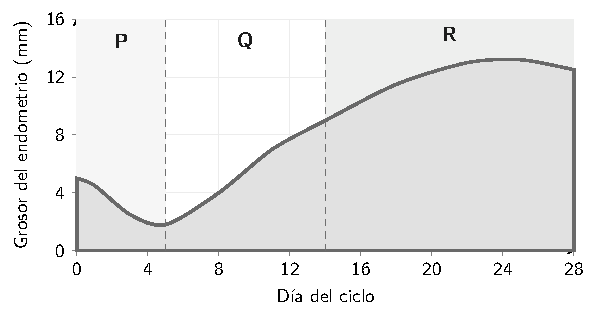
\includegraphics[max width=0.92\linewidth,max height=8.5cm]{bio/rep_endometrio}
\end{center}
 
\begin{clave}[{Recuerda}] P es la fase menstrual, Q la proliferativa (estrógeno) y R la secretora (progesterona).\end{clave}
\subsection{Quién regula a quién}
El ciclo se controla con un \textbf{eje hormonal}:

 
\begin{enumerate}
  \item El \textbf{hipotálamo} libera \textbf{GnRH}.
  \item La GnRH estimula a la \textbf{hipófisis anterior}, que libera \textbf{FSH} y \textbf{LH}.
  \item FSH y LH actúan sobre el \textbf{ovario}, que produce \textbf{estrógeno} y \textbf{progesterona}.
  \item Estas hormonas actúan sobre el \textbf{endometrio} y, además, vuelven al hipotálamo y a la hipófisis.
\end{enumerate}
 

\textbf{Retroalimentación negativa:} cuando el estrógeno y la progesterona están altos, frenan la liberación de GnRH, FSH y LH. Por eso en la fase lútea no maduran nuevos folículos, y por eso funcionan las píldoras anticonceptivas.

 

\textbf{Retroalimentación positiva:} a mitad del ciclo, un nivel alto y sostenido de estrógeno hace lo contrario: provoca el \textbf{pico de LH} que desencadena la ovulación.

  
\begin{center}
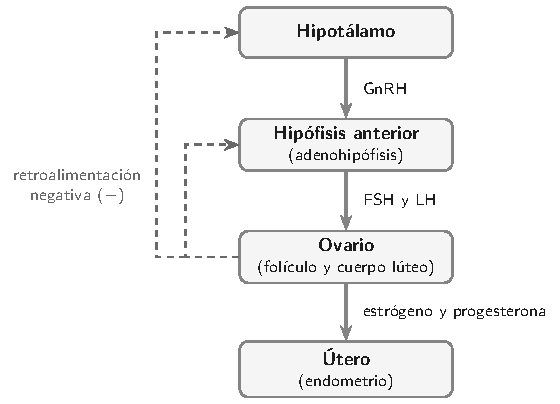
\includegraphics[max width=0.92\linewidth,max height=8.5cm]{bio/rep_eje}
\end{center}
 
\begin{clave}[{Recuerda}] Si el ovario deja de producir hormonas (por ejemplo, en la menopausia), desaparece el freno y la FSH y la LH \textbf{suben}.\end{clave}
\subsection{Leer el gráfico completo}
\begin{center}
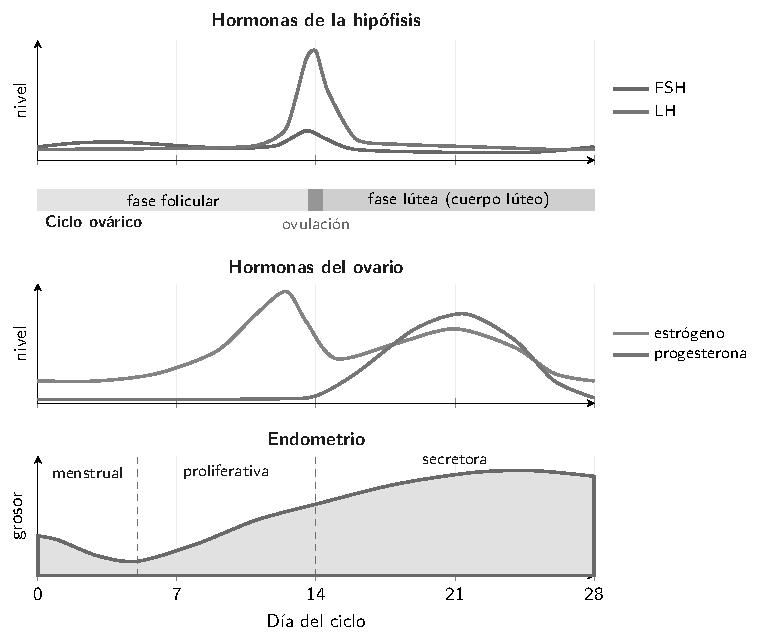
\includegraphics[max width=0.92\linewidth,max height=8.5cm]{bio/rep_ciclo_hormonas}
\end{center}
  

Para leer un gráfico del ciclo, recorre los días de izquierda a derecha y pregúntate qué hormona sube y qué efecto tiene:

 
\begin{itemize}
  \item \textbf{Días 1 a 5:} hormonas ováricas bajas; el endometrio se desprende.
  \item \textbf{Días 6 a 13:} la FSH hace crecer el folículo; el estrógeno sube y engrosa el endometrio.
  \item \textbf{Día 14:} el estrógeno alto provoca el pico de LH; ocurre la ovulación.
  \item \textbf{Días 15 a 25:} el cuerpo lúteo produce progesterona; el endometrio está en fase secretora.
  \item \textbf{Días 25 a 28:} si no hubo embarazo, el cuerpo lúteo degenera, la progesterona cae y comienza una nueva menstruación.
\end{itemize}
 
\begin{clave}[{Pistas rápidas}] Un pico agudo y breve a mitad del ciclo es la LH. La hormona que solo sube después de la ovulación es la progesterona. La que tiene dos subidas, una antes y otra después de la ovulación, es el estrógeno.\end{clave}
\subsection{¿Y si hay fecundación?}
\textbf{Sin fecundación:} el cuerpo lúteo degenera al final del ciclo, la progesterona y el estrógeno caen, el endometrio se desprende (menstruación) y, sin el freno hormonal, la FSH vuelve a subir para iniciar otro ciclo.

 

\textbf{Con fecundación:} el embrión se implanta y produce \textbf{hCG}. La hCG mantiene vivo el \textbf{cuerpo lúteo}, que sigue secretando progesterona. Así el endometrio se mantiene, \textbf{no hay menstruación} y no maduran nuevos folículos. Desde el segundo o tercer mes, la \textbf{placenta} asume la producción de progesterona.

  
\begin{center}
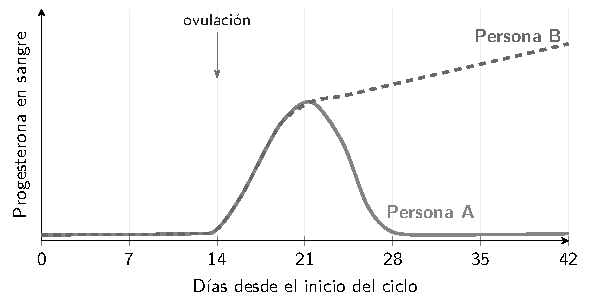
\includegraphics[max width=0.92\linewidth,max height=8.5cm]{bio/rep_embarazo}
\end{center}
 
\begin{clave}[{Recuerda}] En el gráfico, la persona B está embarazada: la hCG mantiene el cuerpo lúteo y la progesterona sigue alta.\end{clave}
\subsection{Lo clave del tema}
\begin{center}\small
\begin{tabularx}{\linewidth}{@{}>{\raggedright\arraybackslash\hsize=0.52\hsize}X>{\raggedright\arraybackslash\hsize=1.15\hsize}X>{\raggedright\arraybackslash\hsize=1.39\hsize}X>{\raggedright\arraybackslash\hsize=0.94\hsize}X@{}}
\toprule
\textbf{Hormona} & \textbf{La produce} & \textbf{Efecto principal} & \textbf{Cuándo está alta} \\
\midrule
GnRH & hipotálamo & estimula la liberación de FSH y LH & todo el ciclo, en pulsos \\
FSH & hipófisis anterior & crecimiento de los folículos & inicio de la fase folicular \\
LH & hipófisis anterior & ovulación y formación del cuerpo lúteo & pico cerca del día 14 \\
Estrógeno & folículo (y cuerpo lúteo) & engrosa el endometrio (fase proliferativa) & antes de la ovulación \\
Progesterona & cuerpo lúteo (luego, la placenta) & prepara y mantiene el endometrio (fase secretora) & fase lútea \\
hCG & embrión implantado & mantiene el cuerpo lúteo & inicio del embarazo \\
\bottomrule
\end{tabularx}
\end{center}
 
\begin{clave}[{Recuerda}] · El pico de LH provoca la ovulación.\par · La caída de progesterona provoca la menstruación.\par · La ovulación ocurre unos 14 días antes de la siguiente menstruación.\par · Estrógeno y progesterona altos frenan la FSH y la LH; si bajan, la FSH y la LH suben.\end{clave}
 
\begin{clave}[{Método PAES}] 1. Ubica el día o la fase del ciclo de la que habla la pregunta. 2. Identifica qué estructura está activa (folículo o cuerpo lúteo) y qué hormona produce. 3. Sigue la cadena: hipotálamo \ensuremath{\rightarrow} hipófisis \ensuremath{\rightarrow} ovario \ensuremath{\rightarrow} endometrio, y recuerda que las hormonas del ovario frenan a las de arriba. 4. Si cambia la duración del ciclo, cuenta 14 días hacia atrás desde la siguiente menstruación.\end{clave}
\begin{elejemplo}{PAES Regular 2026, adaptada}
En una clase de biología se presenta el siguiente gráfico con la concentración en sangre de dos hormonas producidas por el ovario a lo largo de un ciclo de 28 días sin embarazo:

¿Qué hormona es Y y qué estructura del ovario la produce principalmente?
\begin{center}
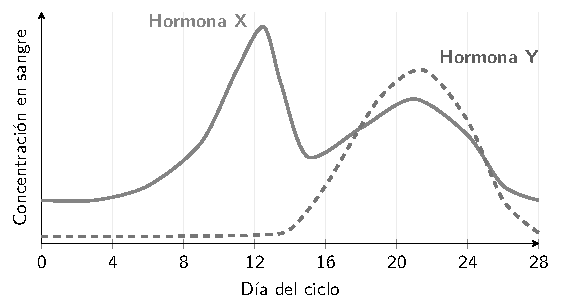
\includegraphics[max width=0.92\linewidth,max height=8.5cm]{bio/rep_ciclo_xy}
\end{center}
\altslargas{Estrógeno, producido por el folículo en crecimiento.}{Progesterona, producida por el cuerpo lúteo.}{LH, producida por la hipófisis.}{Progesterona, producida por el folículo maduro antes de la ovulación.}
\solucion{\textbf{Paso 1. ¿Qué nos piden?} Identificar la hormona Y por la forma de su curva y decir qué estructura la produce.

\textbf{Paso 2. Lee la curva Y.} Está baja durante toda la primera mitad del ciclo, sube \textbf{solo después del día 14}, llega a su máximo cerca del día 21 y cae al final.

\textbf{Paso 3. Relaciona con el ovario.} Después de la ovulación, el folículo roto se transforma en \textbf{cuerpo lúteo}, que secreta progesterona. Cuando el cuerpo lúteo degenera (si no hay embarazo), la progesterona cae. Esa es exactamente la forma de Y.

\textbf{Respuesta:} Y es progesterona, producida por el cuerpo lúteo.

\textbf{¿Por qué no las otras?} El estrógeno es X: sube antes de la ovulación, producido por el folículo en crecimiento. La LH no la produce el ovario y su curva es un pico agudo y breve cerca del día 14. Antes de la ovulación todavía no existe el cuerpo lúteo y la progesterona está baja.

\textbf{\color{cienciaD}Para recordar.} La hormona que solo sube después de la ovulación es la progesterona del cuerpo lúteo.}{B}
\end{elejemplo}
\motivacion{FSH, LH, estrógeno y progesterona: ordenar el ciclo hormonal pide precisión, y tú la tienes.}

%% =====================================================================
%% bio_natalidad
\section[Control de la natalidad e ITS]{Control de la natalidad e ITS}
\modcomun\ \ {\color{gris}\itshape Cómo actúan los métodos naturales (Billings, calendario y temperatura basal), los artificiales reversibles (hormonales y de barrera) y los quirúrgicos (vasectomía y ligadura), cuál protege de las ITS, y las características del VIH, el herpes, la gonorrea y la clamidia.\par}
\subsection{Los métodos y cómo se clasifican}
\begin{center}
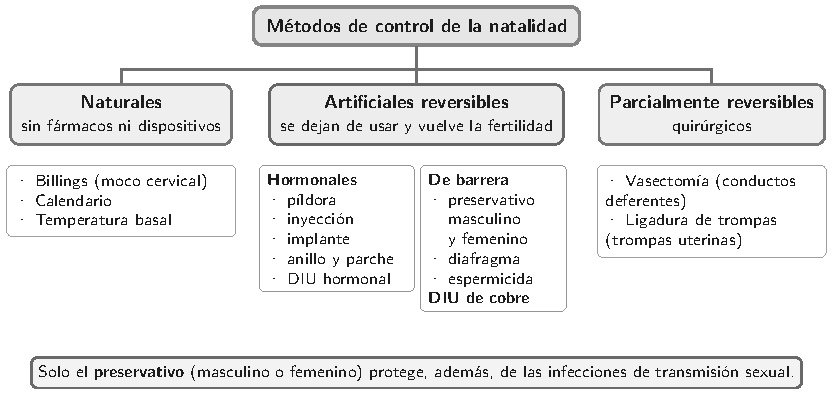
\includegraphics[max width=0.92\linewidth,max height=8.5cm]{bio/rep_metodos}
\end{center}
  

Los métodos de control de la natalidad permiten decidir si tener hijos y cuándo. Todos actúan sobre algún paso de la reproducción:

 
\begin{itemize}
  \item \textbf{impedir la ovulación} (hormonales);
  \item \textbf{impedir que los gametos se encuentren} (barrera, DIU de cobre, quirúrgicos, naturales);
  \item \textbf{dificultar la implantación} o el paso de espermatozoides por el moco cervical (efecto adicional de algunos hormonales).
\end{itemize}
  
\begin{clave}[{Recuerda}] · La \textbf{eficacia} depende del método y también de usarlo bien y siempre.\par · El único método que, además de prevenir el embarazo, protege de las ITS es el \textbf{preservativo}. Por eso se recomienda usarlo siempre, incluso junto a otro método (doble protección).\par · Elegir un método es una decisión informada y compartida, idealmente con orientación de un profesional de la salud.\end{clave}
\subsection{Métodos naturales}
Se basan en reconocer los \textbf{días fértiles} del ciclo y evitar las relaciones sexuales con penetración en esos días. Recuerda que los espermatozoides pueden vivir hasta unos 5 días en el sistema femenino y el ovocito, cerca de un día: los días fértiles van desde unos 5 días antes de la ovulación hasta el día siguiente a ella.

 
\begin{itemize}
  \item \textbf{Billings (moco cervical):} cerca de la ovulación el moco es abundante, transparente y elástico, como clara de huevo. Después se vuelve escaso y espeso.
  \item \textbf{Calendario (Ogino-Knaus):} se registran varios ciclos y se calcula cuándo ocurre la ovulación (unos 14 días antes de la siguiente menstruación).
  \item \textbf{Temperatura basal:} se mide al despertar, antes de levantarse. Después de la ovulación sube entre 0,3 y 0,5 °C por la progesterona y se mantiene alta hasta la menstruación.
\end{itemize}
  
\begin{center}
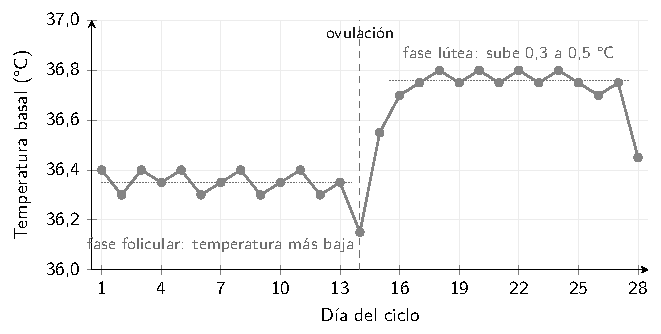
\includegraphics[max width=0.92\linewidth,max height=8.5cm]{bio/rep_temp_basal}
\end{center}
 
\begin{clave}[{Recuerda}] Son métodos de baja eficacia en el uso real, funcionan mejor con ciclos regulares y no protegen de las ITS. El alza de temperatura confirma que la ovulación \textbf{ya ocurrió}; no la anuncia antes.\end{clave}
\subsection{Métodos hormonales}
Contienen hormonas sintéticas parecidas al estrógeno y a la progesterona (progestinas): \textbf{píldora}, \textbf{inyección}, \textbf{implante subdérmico}, \textbf{anillo vaginal}, \textbf{parche} y \textbf{DIU hormonal}.

 

\textbf{Cómo actúan:}

 
\begin{enumerate}
  \item Mantienen altas estas hormonas y, por \textbf{retroalimentación negativa}, frenan la FSH y la LH: no madura un folículo y no hay pico de LH, así que \textbf{no hay ovulación}.
  \item Espesan el \textbf{moco cervical}, lo que dificulta el paso de los espermatozoides.
  \item Modifican el endometrio.
\end{enumerate}
 

Son muy eficaces y reversibles: al dejarlos, la fertilidad vuelve. Requieren indicación y control de salud.

  
\begin{clave}[{Anticoncepción de emergencia}] Es una dosis de hormona que se toma lo antes posible después de una relación sin protección (idealmente dentro de 72 horas). Retrasa o impide la ovulación. No interrumpe un embarazo ya implantado y no reemplaza a un método regular.\end{clave}
 
\begin{clave}[{Recuerda}] Ningún método hormonal protege de las ITS.\end{clave}
\subsection{Métodos de barrera y DIU}
\begin{itemize}
  \item \textbf{Preservativo masculino (condón):} funda de látex u otro material que se coloca sobre el pene erecto. Retiene el semen. Protege del embarazo y de las ITS.
  \item \textbf{Preservativo femenino:} funda que se coloca dentro de la vagina. También protege de las ITS.
  \item \textbf{Diafragma:} copa flexible que cubre el cuello uterino; se usa con espermicida.
  \item \textbf{Espermicida:} sustancia química que inmoviliza o destruye a los espermatozoides.
  \item \textbf{DIU de cobre:} dispositivo que se coloca dentro del útero; el cobre es tóxico para los espermatozoides e impide la fecundación. Dura varios años y se retira cuando se desea.
\end{itemize}
  
\begin{clave}[{Para usar bien el preservativo}] · Revisar la fecha de vencimiento y que el envase esté intacto.\par · Ponerlo desde el inicio de la relación, no solo antes de eyacular.\par · Usar uno nuevo en cada relación y solo uno a la vez.\par · Con lubricante, usar uno a base de agua si es de látex.\end{clave}
\subsection{Métodos quirúrgicos}
\begin{center}
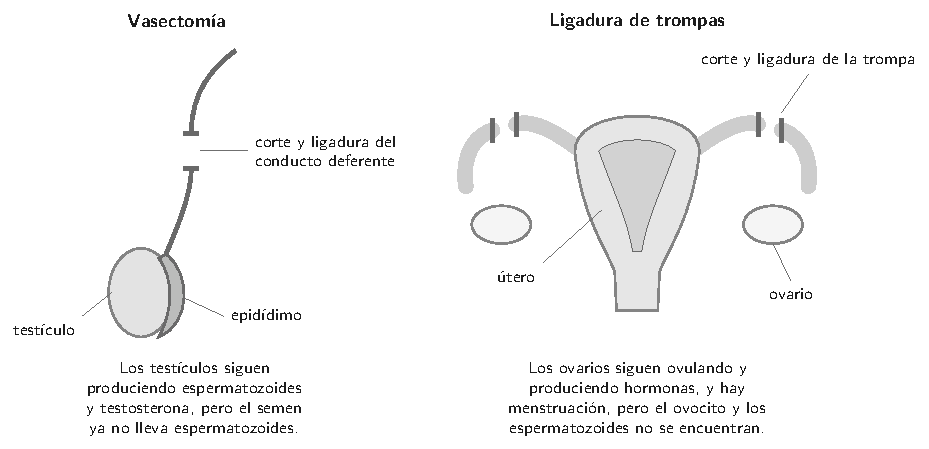
\includegraphics[max width=0.92\linewidth,max height=8.5cm]{bio/rep_quirurgicos}
\end{center}
  

\textbf{Vasectomía:} se cortan y ligan los \textbf{conductos deferentes}. Los testículos siguen produciendo espermatozoides (que el cuerpo reabsorbe) y testosterona; la erección y la eyaculación no cambian, pero el semen ya no lleva espermatozoides. No es inmediata: hay que esperar unos meses y confirmarlo con un examen de semen.

  

\textbf{Ligadura de trompas:} se cortan, ligan o bloquean las \textbf{trompas uterinas}. Los ovarios siguen ovulando y produciendo hormonas, y la menstruación continúa, pero el ovocito y los espermatozoides no se encuentran.

 
\begin{clave}[{Recuerda}] Se consideran \textbf{definitivos}. Se clasifican como parcialmente reversibles porque una cirugía puede reconectar los conductos, pero no siempre se recupera la fertilidad. No protegen de las ITS.\end{clave}
\subsection{Infecciones de transmisión sexual (ITS)}
\begin{center}\small
\begin{tabularx}{\linewidth}{@{}>{\raggedright\arraybackslash\hsize=0.42\hsize}X>{\raggedright\arraybackslash\hsize=0.96\hsize}X>{\raggedright\arraybackslash\hsize=1.20\hsize}X>{\raggedright\arraybackslash\hsize=1.20\hsize}X>{\raggedright\arraybackslash\hsize=1.20\hsize}X@{}}
\toprule
\textbf{ITS} & \textbf{Agente} & \textbf{Transmisión} & \textbf{Síntomas generales} & \textbf{Tratamiento} \\
\midrule
VIH / sida & virus (retrovirus) & relaciones sexuales, sangre (jeringas compartidas), de madre a hijo en el embarazo, parto o lactancia & puede pasar años sin síntomas; destruye linfocitos T CD4 y debilita el sistema inmune; el sida es su etapa avanzada, con infecciones oportunistas & antirretrovirales: no curan, pero controlan el virus; con carga viral indetectable no se transmite por vía sexual \\
Herpes genital & virus (VHS-2 y también VHS-1) & contacto de piel o mucosas con la zona infectada & vesículas y úlceras dolorosas que reaparecen; el virus queda latente en el cuerpo & antivirales que reducen los brotes; no hay cura \\
Gonorrea & bacteria (\emph{Neisseria gonorrhoeae}) & relaciones sexuales & secreción con pus y ardor al orinar; a menudo sin síntomas, sobre todo en mujeres; puede causar infertilidad & antibióticos \\
Clamidia & bacteria (\emph{Chlamydia trachomatis}) & relaciones sexuales & con frecuencia sin síntomas; secreción o dolor; si no se trata, daña las trompas y puede causar infertilidad & antibióticos \\
\bottomrule
\end{tabularx}
\end{center}
 
\begin{clave}[{Prevención}] Usar preservativo en todas las relaciones, hacerse exámenes periódicos (muchas ITS no dan síntomas), conversar con la pareja, no compartir jeringas y consultar ante cualquier síntoma. Las ITS bacterianas se curan con antibióticos; las virales no responden a antibióticos.\end{clave}
\subsection{Lo clave del tema}
\begin{center}\small
\begin{tabularx}{\linewidth}{@{}>{\raggedright\arraybackslash\hsize=1.21\hsize}X>{\raggedright\arraybackslash\hsize=1.21\hsize}X>{\raggedright\arraybackslash\hsize=1.09\hsize}X>{\raggedright\arraybackslash\hsize=0.48\hsize}X@{}}
\toprule
\textbf{Método} & \textbf{Cómo actúa} & \textbf{Clasificación} & \textbf{¿Protege de ITS?} \\
\midrule
Billings, calendario, temperatura basal & evitar las relaciones en los días fértiles & natural & no \\
Píldora, inyección, implante, anillo, parche & impiden la ovulación (frenan FSH y LH) y espesan el moco & artificial reversible (hormonal) & no \\
Preservativo masculino y femenino & retiene el semen: los gametos no se encuentran & artificial reversible (barrera) & \textbf{sí} \\
Diafragma y espermicida & barrera en el cuello uterino; inmoviliza espermatozoides & artificial reversible (barrera) & no \\
DIU de cobre & el cobre afecta a los espermatozoides & artificial reversible & no \\
Vasectomía y ligadura & cortan los conductos deferentes o las trompas & parcialmente reversible (quirúrgico) & no \\
\bottomrule
\end{tabularx}
\end{center}
 
\begin{clave}[{Recuerda}] · VIH y herpes son virus; gonorrea y clamidia, bacterias.\par · Muchas ITS no dan síntomas: el examen es la única forma de saberlo.\par · La vasectomía y la ligadura no cambian las hormonas ni la menstruación.\end{clave}
 
\begin{clave}[{Método PAES}] 1. Ubica qué paso de la reproducción bloquea el método (ovulación, encuentro de los gametos o implantación). 2. Para ITS, identifica el agente: bacteria (antibióticos) o virus (antivirales). 3. En tablas y gráficos, compara por grupos y concluye solo lo que muestran los datos. 4. En preguntas de investigación, busca qué se mide y qué se compara.\end{clave}
\begin{elejemplo}{Estilo PAES}
Una persona registra cada mañana, al despertar, su temperatura basal durante un ciclo de 28 días. Obtiene el siguiente gráfico:

¿Qué indica el alza sostenida de la temperatura desde el día 15?
\begin{center}
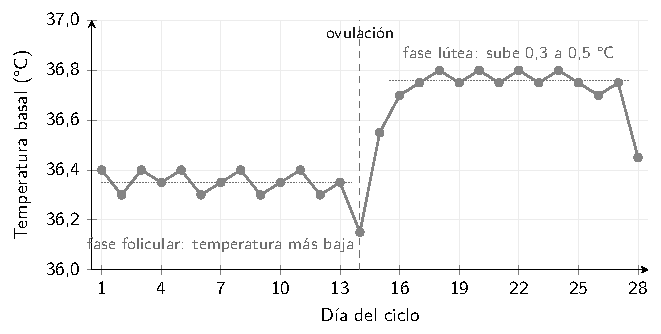
\includegraphics[max width=0.92\linewidth,max height=8.5cm]{bio/rep_temp_basal}
\end{center}
\altslargas{Que la ovulación ocurrirá en los próximos días.}{Que comenzó la menstruación.}{Que la persona tiene una infección.}{Que la ovulación ya ocurrió y el cuerpo lúteo está secretando progesterona.}
\solucion{\textbf{Paso 1. ¿Qué nos piden?} Interpretar el cambio de temperatura en la segunda mitad del ciclo.

\textbf{Paso 2. Recuerda la causa.} Después de la ovulación se forma el cuerpo lúteo, que secreta progesterona. La progesterona sube la temperatura basal entre 0,3 y 0,5 °C, y se mantiene alta mientras el cuerpo lúteo funciona.

\textbf{Paso 3. Lee el gráfico.} La temperatura se mantiene baja hasta el día 14 y sube desde el día 15 hasta casi el final: la ovulación ocurrió cerca del día 14.

\textbf{Respuesta:} que la ovulación ya ocurrió y el cuerpo lúteo está secretando progesterona.

\textbf{¿Por qué no las otras?} El alza aparece \textbf{después} de la ovulación, no antes: por eso este método confirma la ovulación, pero no la anticipa. La menstruación ocurre cuando la progesterona baja, y en el gráfico corresponde a la caída del día 28. Una fiebre por infección no forma este patrón de dos niveles que se repite en cada ciclo.

\textbf{\color{cienciaD}Para recordar.} El alza de la temperatura basal confirma que la ovulación ya ocurrió (efecto de la progesterona).}{D}
\end{elejemplo}
\motivacion{Conocer los métodos anticonceptivos y las ITS es cuidar tu salud y la de los demás. Este tema sirve para la prueba y para la vida.}

\chapter{Herencia y evolución}
%% =====================================================================
%% bio_ciclo_celular
\section[Cromatina y ciclo celular]{Cromatina y ciclo celular}
\modcomun\ \ {\color{gris}\itshape Cómo se empaqueta el ADN (nucleosomas, fibra, cromosoma, cromátidas hermanas y centrómero), las etapas del ciclo celular (G1, S, G2 y fase M), sus puntos de control y el cáncer como pérdida de control.\par}
\subsection{La cromatina y sus grados de compactación}
Una célula humana tiene cerca de \textbf{2 metros} de ADN dentro de un núcleo de unos 6 micrómetros. Cabe porque el ADN no está suelto: se enrolla en proteínas llamadas \textbf{histonas}. El conjunto de ADN e histonas es la \textbf{cromatina}.

 

La cromatina tiene varios \textbf{grados de compactación}:

 
\begin{itemize}
  \item \textbf{Nucleosoma:} un tramo de ADN da casi dos vueltas alrededor de un grupo de ocho histonas. Una hilera de nucleosomas parece un «collar de perlas».
  \item \textbf{Fibra de cromatina:} los nucleosomas se pliegan y se acercan entre sí.
  \item \textbf{Cromosoma:} la fibra forma bucles y se pliega más. Al dividirse la célula alcanza su \textbf{máxima compactación} y se ve al microscopio.
\end{itemize}
  
\begin{clave}[{¿Por qué cambia la compactación?}] En la interfase la cromatina está más \textbf{descondensada}: así las enzimas pueden leer los genes y replicar el ADN. Al dividirse, la cromatina se \textbf{condensa} al máximo: así los cromosomas se reparten entre las células hijas sin enredarse ni cortarse.\end{clave}
 
\begin{clave}[{Recuerda}] Cromatina y cromosoma son el mismo material (ADN con histonas) en distinto grado de compactación.\end{clave}
  
\begin{center}
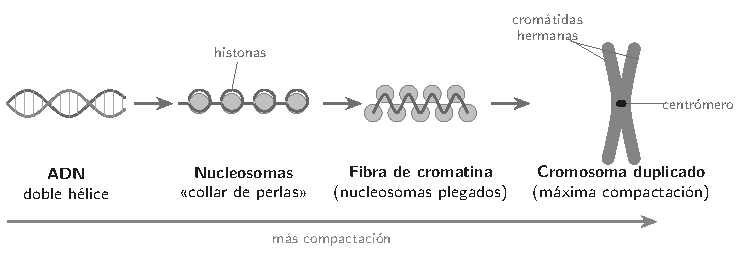
\includegraphics[max width=0.92\linewidth,max height=8.5cm]{bio/div_compactacion}
\end{center}
\subsection{Cromosomas, cromátidas y centrómero}
Antes de dividirse, la célula \textbf{copia su ADN}. Desde ese momento cada cromosoma tiene dos \textbf{cromátidas hermanas}: dos moléculas de ADN idénticas, unidas por el \textbf{centrómero}. Es un cromosoma \textbf{duplicado}.

 

Cuando las cromátidas hermanas se separan, cada una pasa a ser un cromosoma \textbf{simple} (de una cromátida).

 

\textbf{Cromosomas homólogos.} Las células del cuerpo son \textbf{diploides (2n)}: tienen pares de cromosomas, uno heredado de la madre y otro del padre. Los dos cromosomas de un par son \textbf{homólogos}: llevan los mismos genes en el mismo orden, pero pueden tener versiones distintas (alelos). En el ser humano, 2n = 46: 23 pares.

  
\begin{clave}[{Cómo contar}] · Número de \textbf{cromosomas} = número de \textbf{centrómeros}.\par · Cada cromosoma duplicado aporta \textbf{dos cromátidas} (dos moléculas de ADN).\par · Cada cromosoma simple aporta \textbf{una cromátida}.\end{clave}
 
\begin{center}\small
\begin{tabular}{@{}lll@{}}
\toprule
\textbf{Célula humana} & \textbf{Cromosomas} & \textbf{Cromátidas} \\
\midrule
En G1 (antes de replicar) & 46 & 46 \\
En G2 (después de replicar) & 46 & 92 \\
\bottomrule
\end{tabular}
\end{center}
 
\begin{clave}[{Recuerda}] Las cromátidas hermanas son \textbf{copias idénticas} que vienen de la replicación. Los homólogos son \textbf{dos cromosomas distintos}, uno de cada progenitor.\end{clave}
\subsection{Las etapas del ciclo celular}
El \textbf{ciclo celular} es la secuencia de etapas que vive una célula desde que se forma hasta que se divide en dos. Tiene dos grandes partes:

 

\textbf{Interfase} (la más larga, en muchas células más del 90 \% del ciclo):

 
\begin{itemize}
  \item \textbf{G1:} la célula crece, fabrica proteínas y organelos y cumple su función.
  \item \textbf{S:} síntesis (replicación) del ADN. Cada cromosoma queda con dos cromátidas.
  \item \textbf{G2:} la célula sigue creciendo y se prepara para dividirse.
\end{itemize}
 

\textbf{Fase M:} la \textbf{mitosis} (reparto del núcleo) y la \textbf{citocinesis} (reparto del citoplasma).

 

Algunas células salen del ciclo desde G1 a un estado de reposo llamado \textbf{G0}: siguen vivas y funcionando, pero no se dividen. Ejemplos: la mayoría de las neuronas y las células del músculo cardíaco.

  
\begin{center}
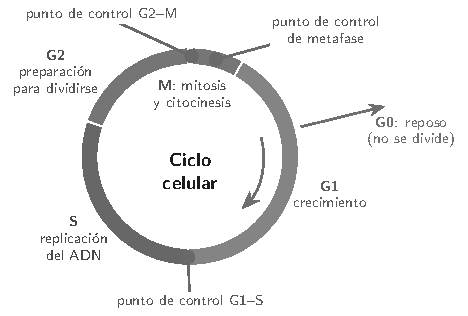
\includegraphics[max width=0.92\linewidth,max height=8.5cm]{bio/div_ciclo}
\end{center}
\subsection{Los puntos de control}
El ciclo no avanza «a ciegas». En ciertos momentos, proteínas de control revisan si todo está en orden. Si algo falla, el ciclo \textbf{se detiene} hasta que se corrige; si el daño no tiene arreglo, la célula activa la \textbf{apoptosis} (muerte celular programada).

 
\begin{center}\small
\begin{tabularx}{\linewidth}{@{}>{\raggedright\arraybackslash\hsize=0.57\hsize}X>{\raggedright\arraybackslash\hsize=1.43\hsize}X@{}}
\toprule
\textbf{Punto de control} & \textbf{Qué revisa} \\
\midrule
G1--S & tamaño celular, nutrientes, señales para dividirse y ADN sin daño, antes de replicarlo \\
G2--M & ADN replicado por completo y sin daño, antes de entrar en mitosis \\
Metafase & todos los cromosomas unidos al huso mitótico, antes de separar las cromátidas \\
\bottomrule
\end{tabularx}
\end{center}
  
\begin{ejemplo}[{Ejemplo resuelto}] Se trata un cultivo con un fármaco que impide armar el huso mitótico. Los cromosomas no logran unirse al huso, así que el punto de control de metafase no deja pasar a la anafase: las células se \textbf{acumulan en metafase}. Así actúan algunos fármacos contra el cáncer y así se preparan las células para fotografiar cromosomas.\end{ejemplo}
 
\begin{clave}[{Recuerda}] Cada punto de control revisa lo que acaba de pasar y deja avanzar solo si está bien: antes de replicar (G1--S), antes de dividir (G2--M) y antes de separar (metafase).\end{clave}
\subsection{Cáncer: cuando se pierde el control}
Los puntos de control dependen de genes. Hay dos grupos importantes:

 
\begin{itemize}
  \item \textbf{Protooncogenes:} codifican proteínas que estimulan la división, como un acelerador. Si mutan y quedan siempre activos (\textbf{oncogenes}), la célula recibe la orden de dividirse sin parar.
  \item \textbf{Genes supresores de tumores:} codifican proteínas que frenan el ciclo o activan la apoptosis, como el freno. El más conocido es \textbf{p53}, que detiene el ciclo en G1 si el ADN está dañado. Si se pierde, las células con ADN dañado siguen dividiéndose.
\end{itemize}
 

El \textbf{cáncer} aparece cuando se acumulan mutaciones en estos genes: las células se dividen sin control y forman un \textbf{tumor}. Si invaden otros tejidos y viajan por la sangre o la linfa, hay \textbf{metástasis}.

  
\begin{clave}[{Factores de riesgo}] Todo lo que daña el ADN aumenta el riesgo: radiación UV, humo de tabaco, algunos virus (como el VPH) y ciertas sustancias químicas. También influyen la edad y la herencia.\end{clave}
 
\begin{clave}[{Tratamientos}] La quimioterapia y la radioterapia atacan sobre todo a las células que se dividen rápido. Por eso también afectan a tejidos sanos que se dividen mucho, como la raíz del pelo y la mucosa del intestino.\end{clave}
\subsection{Lo clave del tema}
\begin{center}\small
\begin{tabularx}{\linewidth}{@{}>{\raggedright\arraybackslash\hsize=0.60\hsize}X>{\raggedright\arraybackslash\hsize=1.20\hsize}X>{\raggedright\arraybackslash\hsize=1.20\hsize}X@{}}
\toprule
\textbf{Etapa} & \textbf{Qué ocurre} & \textbf{Cromosomas} \\
\midrule
G1 & crecimiento y función & 2n, de una cromátida \\
S & replicación del ADN & 2n, pasan a dos cromátidas \\
G2 & preparación para dividirse & 2n, de dos cromátidas \\
Mitosis & reparto de los cromosomas & 2n \\
Células hijas & vuelven a G1 & 2n, de una cromátida \\
\bottomrule
\end{tabularx}
\end{center}
 
\begin{clave}[{Recuerda}] · En la fase S se replica el ADN: cada cromosoma pasa a tener dos cromátidas, pero el número de cromosomas no cambia.\par · Cromátidas hermanas: copias idénticas unidas por el centrómero. Homólogos: un cromosoma materno y uno paterno.\par · La cromatina está descondensada en interfase y alcanza su máxima compactación en la metafase.\par · Un punto de control detiene el ciclo hasta corregir el problema; si no se puede, la célula muere por apoptosis.\end{clave}
 
\begin{clave}[{Método PAES}] 1. Ubica la etapa: ¿antes o después de replicar? ¿antes o después de dividirse? 2. En un punto de control, pregúntate qué revisa y qué etapa impide comenzar. 3. En un experimento con fármacos, compara con el control: si se acumulan células en una etapa, el fármaco bloquea el paso a la siguiente.\end{clave}
\begin{elejemplo}{PAES Invierno 2026, adaptada}
Para estudiar un nuevo fármaco contra el cáncer, se cultivaron células tumorales en dos condiciones: con y sin el fármaco. Después de 24 horas se midió el porcentaje de células en cada etapa del ciclo celular:

Según estos resultados, ¿cuál es el efecto más probable del fármaco?
\begin{center}
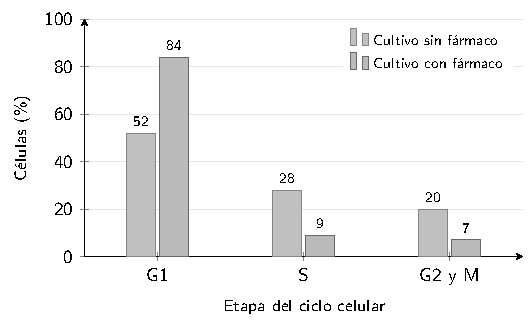
\includegraphics[max width=0.92\linewidth,max height=8.5cm]{bio/div_farmaco}
\end{center}
\altslargas{Acelera la replicación del ADN.}{Bloquea la separación de las cromátidas en la anafase.}{Impide que las células pasen de G1 a la fase S.}{Aumenta el número de células que se dividen.}
\solucion{\textbf{Paso 1. ¿Qué nos piden?} Inferir el efecto del fármaco comparando con el cultivo sin fármaco (control).

\textbf{Paso 2. Compara las barras.} Con el fármaco, las células en G1 suben de 52 \% a 84 \%. Las células en S bajan de 28 \% a 9 \% y las de G2 y M bajan de 20 \% a 7 \%.

\textbf{Paso 3. Interpreta.} Las células se acumulan en G1 y llegan menos a las etapas siguientes: el fármaco frena el paso de G1 a S. Es como si activara el punto de control G1--S.

\textbf{Respuesta:} impide que las células pasen de G1 a la fase S.

\textbf{¿Por qué no las otras?} Si acelerara la replicación no habría menos células en S y más en G1. Si bloqueara la anafase, las células se acumularían en M, pero ese grupo bajó. Hay menos células en S, G2 y M, así que se dividen menos, no más.

\textbf{\color{cienciaD}Para recordar.} Si las células se acumulan en una etapa, el fármaco bloquea el paso a la siguiente.}{C}
\end{elejemplo}
\motivacion{Interfase, cromatina y control del ciclo: ya sabes cómo se prepara una célula para dividirse. Prepárate tú de la misma forma.}

%% =====================================================================
%% bio_mitosis
\section[Mitosis]{Mitosis}
\modcomun\ \ {\color{gris}\itshape Las etapas de la mitosis (profase, metafase, anafase y telofase) y la citocinesis, cómo reconocerlas en un dibujo y su importancia para conservar la información genética, crecer, desarrollarse y reparar tejidos.\par}
\subsection{Qué es la mitosis y para qué sirve}
La \textbf{mitosis} es la división del núcleo que produce \textbf{dos núcleos con la misma información genética} que la célula original. Le sigue la \textbf{citocinesis}, que reparte el citoplasma: el resultado son dos células hijas idénticas entre sí y a la célula madre.

 

Si la célula madre es diploide (2n), las hijas también lo son: \textbf{2n \ensuremath{\rightarrow} 2n}.

 

La mitosis permite:

 
\begin{itemize}
  \item \textbf{Conservar la información genética:} cada célula del cuerpo tiene los mismos cromosomas que el cigoto del que proviene.
  \item \textbf{Crecer y desarrollarse:} de un cigoto se llega a un cuerpo con billones de células.
  \item \textbf{Reparar tejidos:} reemplazar células de la piel, cerrar una herida o soldar un hueso.
  \item \textbf{Reproducirse asexualmente:} levaduras, esquejes de plantas, estolones de la frutilla.
\end{itemize}
  
\begin{clave}[{La clave de la mitosis}] Antes de dividirse, en la fase S, cada cromosoma se copió: tiene dos cromátidas hermanas idénticas. En la mitosis esas cromátidas se separan y \textbf{cada célula hija recibe una copia de cada cromosoma}. Por eso las hijas son idénticas.\end{clave}
 
\begin{clave}[{Recuerda}] La mitosis ocurre en las células del cuerpo (somáticas). Los gametos se forman por meiosis.\end{clave}
\subsection{Profase y metafase}
\textbf{Profase.}

 
\begin{itemize}
  \item La cromatina se \textbf{condensa}: aparecen los cromosomas, cada uno con dos cromátidas hermanas.
  \item Desaparece el nucléolo y la \textbf{envoltura nuclear se desorganiza}.
  \item Los centrosomas (con sus centriolos, en células animales) se van a polos opuestos y entre ellos se arma el \textbf{huso mitótico}, hecho de microtúbulos.
  \item Los microtúbulos se unen a los cromosomas en el centrómero, en unas estructuras de proteína llamadas \textbf{cinetocoros}.
\end{itemize}
  

\textbf{Metafase.}

 
\begin{itemize}
  \item Los cromosomas, con su máxima condensación, se ordenan en el \textbf{plano ecuatorial} de la célula (placa metafásica).
  \item Cada cromátida hermana queda unida a fibras de un polo distinto.
  \item Actúa el \textbf{punto de control de metafase}: la anafase no comienza hasta que todos los cromosomas estén unidos al huso.
\end{itemize}
 
\begin{clave}[{Recuerda}] En la profase y la metafase los cromosomas siguen siendo duplicados: cada uno tiene dos cromátidas hermanas unidas por el centrómero.\end{clave}
\subsection{Anafase, telofase y citocinesis}
\textbf{Anafase.} Se rompen las uniones entre las cromátidas hermanas, que se \textbf{separan} y son arrastradas a polos opuestos por las fibras del huso. Desde ese momento cada cromátida es un cromosoma simple. Es la etapa más corta.

 

\textbf{Telofase.} Los cromosomas llegan a los polos y se \textbf{descondensan}. Se forma una envoltura nuclear alrededor de cada grupo y reaparece el nucléolo: hay dos núcleos.

  

\textbf{Citocinesis.} Se divide el citoplasma:

 
\begin{itemize}
  \item En \textbf{células animales}, un anillo de actina y miosina estrangula la célula desde afuera hacia adentro: el \textbf{surco de segmentación}.
  \item En \textbf{células vegetales}, la pared rígida no deja estrangular: vesículas del aparato de Golgi forman en el centro una \textbf{placa celular} que crece hacia los bordes y da origen a la nueva pared.
\end{itemize}
  
\begin{center}
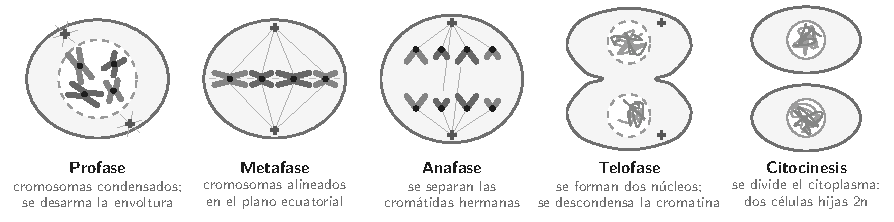
\includegraphics[max width=0.92\linewidth,max height=8.5cm]{bio/div_mitosis}
\end{center}
\subsection{Cómo reconocer cada etapa en un dibujo}
\begin{center}\small
\begin{tabularx}{\linewidth}{@{}>{\raggedright\arraybackslash\hsize=1.29\hsize}X>{\raggedright\arraybackslash\hsize=0.71\hsize}X@{}}
\toprule
\textbf{Si ves\dots{}} & \textbf{La etapa es\dots{}} \\
\midrule
núcleo con envoltura y cromatina sin cromosomas visibles & interfase \\
cromosomas duplicados condensándose; envoltura que se desarma & profase \\
cromosomas duplicados en fila en el centro de la célula & metafase \\
dos grupos de cromosomas simples (en forma de V) que van a los polos & anafase \\
dos núcleos que se reorganizan en los polos; surco o placa celular & telofase y citocinesis \\
\bottomrule
\end{tabularx}
\end{center}
  
\begin{clave}[{Pistas para reconocer}] Mira la forma de los cromosomas: en X tienen dos cromátidas (todavía no se separan); en V o bastón tienen una (ya se separaron). Luego mira dónde están: dispersos en el núcleo, en fila al centro o yendo hacia los polos.\end{clave}
  
\begin{ejemplo}[{Ejemplo resuelto}] En un dibujo hay una célula con dos grupos de cromosomas en forma de V que se alejan hacia polos opuestos. Son cromátidas hermanas que se separan: es una \textbf{anafase}. Cada célula hija recibirá una copia de cada cromosoma.\end{ejemplo}
\subsection{Lo clave del tema}
\begin{center}\small
\begin{tabularx}{\linewidth}{@{}>{\raggedright\arraybackslash\hsize=0.45\hsize}X>{\raggedright\arraybackslash\hsize=1.28\hsize}X>{\raggedright\arraybackslash\hsize=1.28\hsize}X@{}}
\toprule
\textbf{Etapa} & \textbf{Evento principal} & \textbf{Cómo se ven los cromosomas} \\
\midrule
Profase & condensación, se desarma la envoltura, se forma el huso & duplicados (en X), condensándose \\
Metafase & alineación en el plano ecuatorial; punto de control & duplicados (en X), en fila al centro \\
Anafase & separación de las cromátidas hermanas & simples (en V), hacia los polos \\
Telofase & dos núcleos; descondensación & simples, descondensándose en cada núcleo \\
Citocinesis & división del citoplasma (surco o placa celular) & dos células 2n idénticas \\
\bottomrule
\end{tabularx}
\end{center}
 
\begin{clave}[{Recuerda}] · En la anafase de la mitosis se separan las cromátidas hermanas.\par · Las células hijas tienen el mismo número de cromosomas que la madre: 2n \ensuremath{\rightarrow} 2n.\par · La mitosis conserva la información genética: sirve para crecer, desarrollarse, reparar tejidos y reproducirse asexualmente.\end{clave}
 
\begin{clave}[{Método PAES}] 1. Para reconocer una etapa, mira la envoltura nuclear, la posición de los cromosomas y su forma (X o V). 2. En una tabla de duraciones, relaciona cada etapa con su evento. 3. Si un fármaco afecta un componente (huso, actina, cohesión), deduce en qué etapa quedan detenidas las células.\end{clave}
\begin{elejemplo}{PAES Regular 2026, adaptada}
Una profesora muestra a su curso el siguiente esquema, con cuatro células de un mismo tejido en distintas etapas de la mitosis, numeradas al azar:

¿En qué orden ocurren estas etapas?
\begin{center}
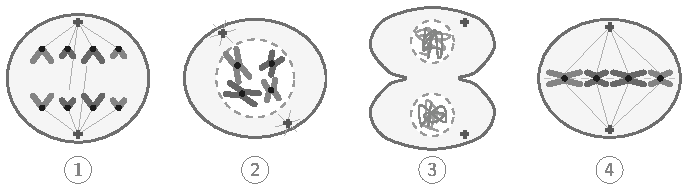
\includegraphics[max width=0.92\linewidth,max height=8.5cm]{bio/div_mitosis_q}
\end{center}
\alts{4, 2, 1 y 3.}{2, 4, 1 y 3.}{2, 1, 4 y 3.}{3, 2, 4 y 1.}
\solucion{\textbf{Paso 1. ¿Qué nos piden?} Ordenar las cuatro células según la secuencia de la mitosis.

\textbf{Paso 2. Identifica cada célula.} Célula 2: cromosomas duplicados condensándose y envoltura que se desarma \ensuremath{\rightarrow} \textbf{profase}. Célula 4: cromosomas duplicados en fila en el centro \ensuremath{\rightarrow} \textbf{metafase}. Célula 1: cromosomas simples en forma de V que van a los polos \ensuremath{\rightarrow} \textbf{anafase}. Célula 3: dos núcleos en formación y la célula estrangulándose \ensuremath{\rightarrow} \textbf{telofase} con citocinesis.

\textbf{Paso 3. Ordena.} Profase, metafase, anafase y telofase: 2, 4, 1 y 3.

\textbf{Respuesta:} 2, 4, 1 y 3.

\textbf{¿Por qué no las otras?} «4, 2, 1 y 3» pone la metafase antes que la profase, pero los cromosomas primero se condensan y después se alinean. «2, 1, 4 y 3» pone la anafase antes que la metafase: las cromátidas solo se separan una vez que todos los cromosomas están alineados. «3, 2, 4 y 1» empieza con la telofase, que es la última etapa.

\textbf{\color{cienciaD}Para recordar.} Profase, metafase, anafase, telofase: condensar, alinear, separar, rehacer los núcleos.}{B}
\end{elejemplo}
\motivacion{Profase, metafase, anafase y telofase: ya las ordenas sin pensarlo. Tu conocimiento también se multiplica.}

%% =====================================================================
%% bio_meiosis
\section[Meiosis y variabilidad genética]{Meiosis y variabilidad genética}
\modcomun\ \ {\color{gris}\itshape Las etapas de la meiosis I y II, el entrecruzamiento y la permutación cromosómica, el paso de células 2n a células n, la comparación con la mitosis y su aporte a la variabilidad genética.\par}
\subsection{Qué es la meiosis y para qué sirve}
La \textbf{meiosis} es la división que forma las células sexuales. Ocurre en las \textbf{células germinales} de las gónadas: en los testículos (espermatozoides) y los ovarios (ovocitos). En las plantas ocurre en las anteras y en los óvulos de la flor.

 

Tiene tres rasgos que la definen:

 
\begin{itemize}
  \item Una sola replicación del ADN, seguida de \textbf{dos divisiones}: meiosis I y meiosis II.
  \item Reduce a la mitad el número de cromosomas: de una célula \textbf{2n} salen células \textbf{n} (haploides), con un cromosoma de cada par.
  \item Las cuatro células que produce son \textbf{genéticamente distintas} entre sí y distintas de la célula madre.
\end{itemize}
  
\begin{clave}[{¿Por qué reducir a la mitad?}] En la fecundación se unen dos gametos. Si cada uno fuera 2n, el cigoto sería 4n y el número de cromosomas se duplicaría en cada generación. Con gametos n (en humanos, 23 cromosomas), el cigoto vuelve a ser 2n = 46.\end{clave}
 
\begin{clave}[{Recuerda}] Meiosis: 2n \ensuremath{\rightarrow} n, cuatro células distintas. Fecundación: n + n \ensuremath{\rightarrow} 2n.\end{clave}
\subsection{Meiosis I: se separan los homólogos}
La célula llega a la meiosis con el ADN ya replicado: cada cromosoma tiene dos cromátidas.

 
\begin{itemize}
  \item \textbf{Profase I.} Es la etapa más larga. Los cromosomas se condensan y cada par de \textbf{homólogos se aparea} a lo largo (sinapsis), unidos por el complejo sinaptonémico. Cada par forma un \textbf{bivalente} o tétrada (cuatro cromátidas). Ocurre el \textbf{entrecruzamiento}.
  \item \textbf{Metafase I.} Los \textbf{pares de homólogos} se ubican en el plano ecuatorial, uno a cada lado.
\end{itemize}
  
\begin{itemize}
  \item \textbf{Anafase I.} Se separan los \textbf{cromosomas homólogos} y van a polos opuestos. Las cromátidas hermanas siguen unidas.
  \item \textbf{Telofase I.} Se forman dos células \textbf{haploides (n)}, cada una con un cromosoma de cada par, todavía con dos cromátidas.
\end{itemize}
 
\begin{clave}[{Recuerda}] La meiosis I es la \textbf{división reduccional}: es la que reduce el número de cromosomas de 2n a n.\end{clave}
  
\begin{center}
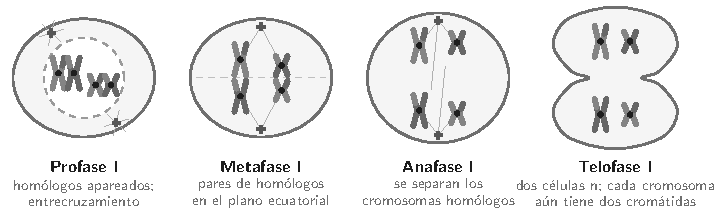
\includegraphics[max width=0.92\linewidth,max height=8.5cm]{bio/div_meiosis1}
\end{center}
\subsection{Meiosis II: se separan las cromátidas}
Entre la meiosis I y la meiosis II \textbf{no hay replicación del ADN}. La meiosis II se parece a una mitosis, pero en células haploides:

 
\begin{itemize}
  \item \textbf{Profase II:} los cromosomas se condensan y se forma un nuevo huso.
  \item \textbf{Metafase II:} los cromosomas, cada uno con dos cromátidas, se alinean en el plano ecuatorial.
  \item \textbf{Anafase II:} se separan las \textbf{cromátidas hermanas} hacia polos opuestos.
  \item \textbf{Telofase II:} se forman los núcleos y se divide el citoplasma.
\end{itemize}
  
\begin{clave}[{Resultado}] De una célula 2n salen \textbf{cuatro células n}, cada una con cromosomas de una cromátida. Gracias al entrecruzamiento, ni siquiera las cromátidas hermanas son ya idénticas: por eso las cuatro células son distintas.\end{clave}
 
\begin{clave}[{Recuerda}] Meiosis I separa homólogos (2n \ensuremath{\rightarrow} n). Meiosis II separa cromátidas hermanas (n \ensuremath{\rightarrow} n).\end{clave}
  
\begin{center}
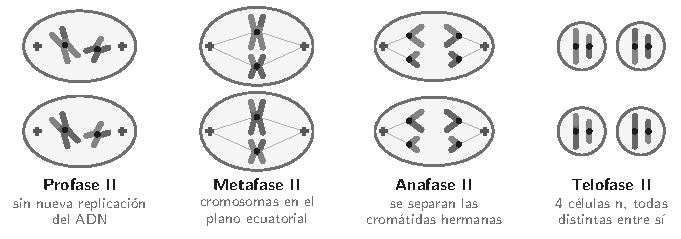
\includegraphics[max width=0.92\linewidth,max height=8.5cm]{bio/div_meiosis2}
\end{center}
\subsection{Entrecruzamiento (crossing-over)}
Durante la profase I, cuando los homólogos están apareados, una cromátida de cada homólogo se corta en el mismo punto y ambas \textbf{intercambian segmentos}. El punto donde quedan unidas se ve como una X y se llama \textbf{quiasma}.

 

Resultado: aparecen \textbf{cromátidas recombinantes}, con una combinación de alelos que no existía en los cromosomas de la madre ni del padre.

 

En el ejemplo, un homólogo tenía los alelos A y B, y el otro, a y b. Tras el entrecruzamiento hay cuatro cromátidas distintas: AB, aB, Ab y ab.

  
\begin{clave}[{Los quiasmas también sirven para repartir bien}] Mantienen unidos a los homólogos hasta la anafase I, para que cada uno vaya a un polo distinto. Si se forman pocos quiasmas, aumenta el riesgo de que un par no se separe (\textbf{no disyunción}) y se formen gametos con un cromosoma de más o de menos.\end{clave}
  
\begin{center}
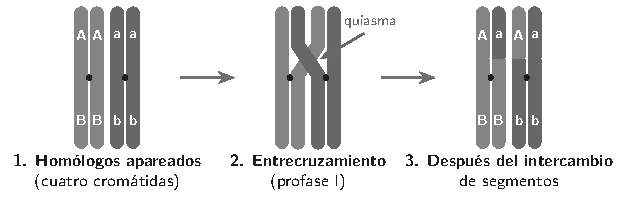
\includegraphics[max width=0.92\linewidth,max height=8.5cm]{bio/div_crossing}
\end{center}
\subsection{Permutación cromosómica y fecundación}
En la metafase I, cada par de homólogos se orienta \textbf{al azar}: el cromosoma materno puede quedar mirando a cualquiera de los dos polos, sin importar cómo se ordenan los otros pares. A esto se le llama \textbf{permutación cromosómica} o segregación independiente.

 

Con n pares de cromosomas hay \textbf{2\textsuperscript{n}} combinaciones posibles de cromosomas en los gametos (sin contar el entrecruzamiento).

 
\begin{itemize}
  \item Con 2 pares: 2\textsuperscript{2} = 4 combinaciones.
  \item En humanos, con 23 pares: 2\textsuperscript{23}, más de 8 millones.
\end{itemize}
  
\begin{center}
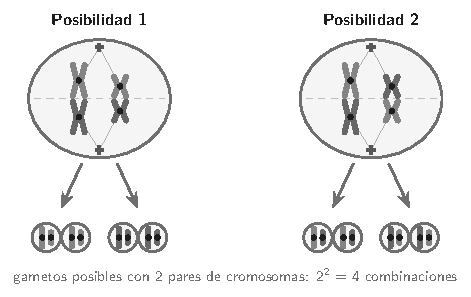
\includegraphics[max width=0.92\linewidth,max height=8.5cm]{bio/div_permutacion}
\end{center}
 
\begin{clave}[{Las fuentes de variabilidad genética}] · \textbf{Mutaciones:} crean alelos nuevos.\par · \textbf{Entrecruzamiento} (profase I): mezcla alelos dentro de un cromosoma.\par · \textbf{Permutación cromosómica} (metafase I): mezcla cromosomas maternos y paternos.\par · \textbf{Fecundación al azar:} cualquier óvulo con cualquier espermatozoide.\end{clave}
\subsection{Lo clave del tema}
\begin{center}\small
\begin{tabularx}{\linewidth}{@{}>{\raggedright\arraybackslash\hsize=0.94\hsize}X>{\raggedright\arraybackslash\hsize=1.12\hsize}X>{\raggedright\arraybackslash\hsize=0.94\hsize}X@{}}
\toprule
 & \textbf{Mitosis} & \textbf{Meiosis} \\
\midrule
Células que la hacen & somáticas & germinales (gónadas) \\
Divisiones & una & dos, tras una sola replicación \\
Células resultantes & 2, diploides (2n), idénticas & 4, haploides (n), distintas \\
Apareamiento y entrecruzamiento & no ocurren & sí, en la profase I \\
Qué se separa en la anafase & cromátidas hermanas & homólogos (I) y cromátidas (II) \\
Función & crecer, reparar, reproducción asexual & formar gametos, variabilidad \\
\bottomrule
\end{tabularx}
\end{center}
 
\begin{clave}[{Recuerda}] · En la anafase I se separan los cromosomas homólogos; en la anafase II, las cromátidas hermanas.\par · Las células que salen de la meiosis I ya son haploides, aunque sus cromosomas tengan dos cromátidas.\par · La variabilidad viene del entrecruzamiento (profase I), la permutación (metafase I) y la fecundación al azar.\end{clave}
 
\begin{clave}[{Método PAES}] 1. En un dibujo, mira qué se mueve hacia los polos: cromosomas en forma de X (homólogos, anafase I) o en forma de V (cromátidas, anafase II o mitosis). 2. Mira cada polo: si tiene pares de homólogos es 2n; si tiene uno de cada tipo es n. 3. Para la variabilidad, usa 2\textsuperscript{n} y suma el entrecruzamiento.\end{clave}
\begin{elejemplo}{PAES Invierno 2026, adaptada}
El siguiente dibujo muestra una célula en división, obtenida del testículo de un animal. Los colores indican el origen de cada cromosoma (materno o paterno):

¿En qué etapa está la célula y cuál es el número diploide de la especie?
\begin{center}
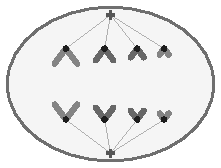
\includegraphics[max width=0.92\linewidth,max height=8.5cm]{bio/div_anafase2_q}
\end{center}
\alts{Anafase de la mitosis; 2n = 4.}{Anafase II de la meiosis; 2n = 8.}{Anafase I de la meiosis; 2n = 8.}{Anafase II de la meiosis; 2n = 4.}
\solucion{\textbf{Paso 1. ¿Qué nos piden?} La etapa de la célula y el número 2n de la especie.

\textbf{Paso 2. ¿Qué se separa?} Los cromosomas tienen forma de V: son cromátidas sueltas. Se están separando cromátidas hermanas: puede ser una mitosis o una anafase II.

\textbf{Paso 3. Mira cada polo.} Cada polo recibe cuatro cromosomas, todos de tamaño distinto: hay \textbf{uno de cada tipo}, sin pares de homólogos. La célula es haploide: es una \textbf{anafase II} y n = 4.

\textbf{Paso 4. Número diploide.} Si n = 4, la especie tiene 2n = 8.

\textbf{Respuesta:} anafase II de la meiosis; 2n = 8.

\textbf{¿Por qué no las otras?} En una mitosis cada polo tendría pares de cromosomas del mismo tamaño. En la anafase I se mueven cromosomas con dos cromátidas (forma de X). 2n = 4 confunde el número de cromosomas de cada polo (4, que es n) con el número diploide.

\textbf{\color{cienciaD}Para recordar.} Cromátidas que se separan y polos sin pares de homólogos: anafase II.}{B}
\end{elejemplo}
\motivacion{La meiosis crea variabilidad, y la variabilidad hace única a cada persona. Tú también tienes tu forma única de aprender.}

%% =====================================================================
%% bio_ingenieria
\section[Manipulación genética]{Manipulación genética}
\modcomun\ \ {\color{gris}\itshape Qué es la manipulación genética, el ADN recombinante y los organismos transgénicos; aplicaciones en alimentos, detergentes, vestuario y fármacos como la insulina humana producida por bacterias; y los beneficios, riesgos y debates que generan.\par}
\subsection{Qué es la manipulación genética}
La \textbf{manipulación genética} (o ingeniería genética) es el conjunto de técnicas que permiten \textbf{modificar el ADN} de un organismo: cortar un gen, copiarlo, cambiarlo o llevarlo de una especie a otra.

 

Cuando se une ADN de dos orígenes distintos (por ejemplo, un gen humano dentro de ADN bacteriano) se obtiene \textbf{ADN recombinante}.

 

Un organismo que lleva en su ADN un gen de \textbf{otra especie} es un \textbf{organismo transgénico} (un tipo de organismo genéticamente modificado, OGM).

  
\begin{clave}[{¿Por qué funciona?}] El \textbf{código genético es universal}: casi todos los seres vivos leen el ADN con las mismas reglas. Por eso una bacteria que recibe el gen humano de la insulina fabrica insulina humana.\end{clave}
 
\begin{clave}[{Recuerda}] Transgénico: tiene un gen de otra especie. Un clon (como la oveja Dolly) es una copia genética de otro individuo, sin genes de otra especie.\end{clave}
\subsection{Aplicaciones}
\begin{center}\small
\begin{tabularx}{\linewidth}{@{}>{\raggedright\arraybackslash\hsize=0.45\hsize}X>{\raggedright\arraybackslash\hsize=1.28\hsize}X>{\raggedright\arraybackslash\hsize=1.28\hsize}X@{}}
\toprule
\textbf{Área} & \textbf{Ejemplo} & \textbf{Cómo se logra} \\
\midrule
Alimentos & maíz y soya resistentes a insectos; arroz dorado con provitamina A & se agrega el gen de la toxina Bt de la bacteria \emph{Bacillus thuringiensis}; genes para fabricar betacaroteno en el grano \\
Detergentes & enzimas que eliminan manchas en agua fría & microorganismos modificados producen en gran cantidad proteasas (proteínas), lipasas (grasas) y amilasas (almidón) \\
Vestuario & algodón Bt & la planta fabrica la toxina Bt y resiste a las larvas que dañan el capullo de fibra; se aplican menos insecticidas \\
Fármacos & insulina humana, hormona del crecimiento, vacuna contra la hepatitis B & bacterias o levaduras con el gen humano producen la proteína \\
\bottomrule
\end{tabularx}
\end{center}
 
\begin{clave}[{Recuerda}] En todas estas aplicaciones el organismo modificado fabrica una proteína nueva porque recibió el gen que la codifica: la toxina Bt, una enzima o una hormona humana.\end{clave}
\subsection{La insulina humana producida por bacterias}
Las personas con diabetes tipo 1 no producen insulina y deben inyectársela. Hasta los años ochenta, la insulina se extraía del páncreas de cerdos y vacas: hacían falta miles de páncreas, y la insulina animal es levemente distinta de la humana.

 

En 1982 se aprobó la primera insulina humana fabricada por bacterias con el gen humano. Fue el primer medicamento obtenido por ingeniería genética.

  
\begin{clave}[{Ventajas}] · Es \textbf{idéntica} a la insulina humana.\par · Se produce en \textbf{grandes cantidades} en fermentadores, sin depender de animales.\par · Su calidad es constante de un lote a otro.\end{clave}
 
\begin{clave}[{Recuerda}] La bacteria no se convierte en célula humana: solo lleva un gen humano y fabrica la proteína que ese gen codifica.\end{clave}
\subsection{Beneficios, riesgos y debates}
\textbf{Beneficios.} Más producción con menos insecticidas, alimentos más nutritivos, medicamentos seguros y abundantes, procesos industriales que ahorran energía y agua.

 

\textbf{Riesgos que se investigan.}

 
\begin{itemize}
  \item Que un gen transgénico pase por polinización a plantas silvestres emparentadas.
  \item Que las plagas se vuelvan resistentes a la toxina Bt.
  \item Que una proteína nueva provoque alergias.
\end{itemize}
  
\begin{clave}[{Ciencia y sociedad}] Algunas preguntas se responden con experimentos (¿pasa el gen a otras plantas?, ¿causa alergia?). Otras dependen de valores y decisiones de la sociedad (¿se deben patentar los seres vivos?, ¿cómo se etiquetan los alimentos?). Ambas son parte del debate, pero se responden de forma distinta.\end{clave}
\subsection{Lo clave del tema}
\begin{center}\small
\begin{tabularx}{\linewidth}{@{}>{\raggedright\arraybackslash\hsize=0.77\hsize}X>{\raggedright\arraybackslash\hsize=1.23\hsize}X@{}}
\toprule
\textbf{Concepto} & \textbf{Qué es} \\
\midrule
Manipulación genética & técnicas para modificar el ADN: cortar un gen, copiarlo o llevarlo de una especie a otra \\
ADN recombinante & ADN formado al unir ADN de dos orígenes distintos \\
Organismo transgénico & lleva en su ADN un gen de otra especie y lo expresa \\
Clon & copia genética de otro individuo, sin genes de otra especie \\
Código genético universal & casi todos los seres vivos leen el ADN con las mismas reglas: por eso una bacteria fabrica una proteína humana \\
\bottomrule
\end{tabularx}
\end{center}
 
\begin{clave}[{Recuerda}] · Un organismo transgénico lleva un gen de otra especie y lo expresa gracias a que el código genético es universal.\par · Un clon o una planta obtenida al cruzar dos variedades de la misma especie no son transgénicos.\par · La insulina producida por bacterias es idéntica a la humana y se fabrica en grandes cantidades.\end{clave}
 
\begin{clave}[{Método PAES}] 1. Para reconocer un transgénico, pregúntate si recibió un gen de otra especie. 2. En las aplicaciones, nombra qué gen se agregó y qué ventaja da. 3. En los detergentes, relaciona cada enzima con lo que digiere: proteasas, proteínas; lipasas, grasas; amilasas, almidón. 4. En un debate, distingue las preguntas que se responden con experimentos de las que dependen de valores.\end{clave}
\begin{elejemplo}{PAES Invierno 2026, adaptada}
El arroz no fabrica betacaroteno (provitamina A) en su grano. Para obtener «arroz dorado», un equipo identificó dos genes, uno de narciso y otro de una bacteria, que codifican las enzimas necesarias para fabricar betacaroteno.

¿Cuál de los siguientes pasos es indispensable para obtener este arroz transgénico?
\altslargas{Regar las plantas de arroz con una solución de betacaroteno.}{Insertar los dos genes en el ADN de células de arroz, de modo que se expresen en el grano.}{Cruzar plantas de arroz con plantas de narciso.}{Inyectar en las semillas las enzimas ya fabricadas por la bacteria.}
\solucion{\textbf{Paso 1. ¿Qué nos piden?} El paso que no puede faltar para obtener un arroz transgénico.

\textbf{Paso 2. Recuerda la definición.} Un organismo transgénico lleva en su \textbf{ADN} genes de otra especie, y los expresa. Para que el arroz fabrique betacaroteno y lo herede a la siguiente generación, los genes deben quedar en el ADN de sus células.

\textbf{Respuesta:} insertar los dos genes en el ADN de células de arroz, de modo que se expresen en el grano.

\textbf{¿Por qué no las otras?} Regar con betacaroteno no cambia el ADN: la planta no aprendería a fabricarlo. Arroz y narciso son especies distintas que no pueden cruzarse. Inyectar las enzimas solo dura hasta que se degraden y no pasa a la descendencia, porque no hay un gen nuevo.

\textbf{\color{cienciaD}Para recordar.} Transgénico: el gen de otra especie se integra en el ADN y se expresa.}{B}
\end{elejemplo}
\motivacion{Transgénicos, clonación y edición genética: ya puedes opinar con fundamentos. Eso es ciencia con criterio.}

%% =====================================================================
%% bio_evidencias
\section[Evidencias de la evolución]{Evidencias de la evolución}
\modcomun\ \ {\color{gris}\itshape Cómo sabemos que las especies evolucionan: anatomía comparada (estructuras homólogas, análogas y vestigiales), embriología, comparación de secuencias de ADN y proteínas, registro fósil y lectura de árboles filogenéticos.\par}
\subsection{La evolución y sus evidencias}
La \textbf{evolución biológica} es el cambio en las características heredables de las \textbf{poblaciones} a lo largo de muchas generaciones. Una de sus ideas centrales es la \textbf{descendencia con modificación}: las especies actuales descienden de especies anteriores, y dos especies cualesquiera comparten, en algún momento del pasado, un \textbf{ancestro común}.

 

Esta idea es una \textbf{teoría científica}: una explicación amplia, puesta a prueba muchas veces y respaldada por evidencias de áreas muy distintas que apuntan a la misma conclusión.

 
\begin{itemize}
  \item \textbf{Anatomía comparada:} se comparan estructuras del cuerpo de especies actuales.
  \item \textbf{Embriología comparada:} se compara el desarrollo de los embriones.
  \item \textbf{Biología molecular:} se comparan secuencias de ADN y de proteínas.
  \item \textbf{Registro fósil:} se estudian restos de organismos del pasado conservados en las rocas.
\end{itemize}
  
\begin{clave}[{La pregunta que se repite}] En todas estas evidencias la PAES pregunta lo mismo: \textbf{¿qué tan emparentadas están estas especies?} Mientras más rasgos compartan por haberlos heredado de un ancestro (huesos, etapas del embrión, secuencias de ADN), más reciente es su ancestro común.\end{clave}
 
\begin{clave}[{Recuerda}] Evolucionan las poblaciones, a lo largo de generaciones. Un individuo no evoluciona durante su vida: crece, aprende o se entrena, pero esos cambios no modifican el ADN de sus gametos.\end{clave}
\subsection{Anatomía comparada: estructuras homólogas}
Las \textbf{estructuras homólogas} tienen el \textbf{mismo origen embrionario} y el \textbf{mismo plan básico}, aunque hoy cumplan funciones distintas.

 

El ejemplo clásico son las extremidades anteriores de los mamíferos. El brazo humano, la pata del gato, la aleta de la ballena y el ala del murciélago sirven para tomar objetos, caminar, nadar y volar, pero todas tienen la misma secuencia de huesos: un \textbf{húmero}, luego \textbf{radio y cúbito}, luego los \textbf{carpos} y al final \textbf{metacarpos y falanges}.

 

Lo que cambia es la forma y el largo de cada hueso: dedos muy largos que sostienen la membrana del ala en el murciélago, huesos cortos y anchos dentro de la aleta en la ballena.

 

\textbf{Qué indican:} que estas especies heredaron ese plan de un \textbf{ancestro común}. A partir de él, cada linaje se fue adaptando a ambientes distintos: es la \textbf{evolución divergente}.

  
\begin{center}
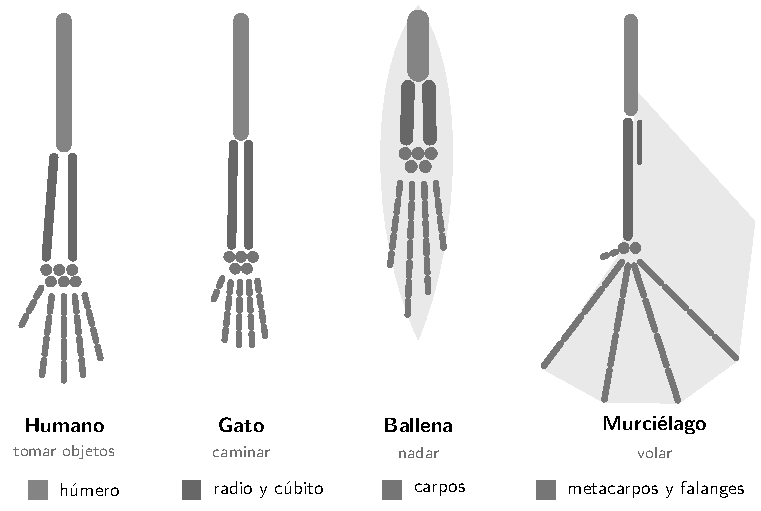
\includegraphics[max width=0.92\linewidth,max height=8.5cm]{bio/evo_extremidades}
\end{center}
\subsection{Estructuras análogas, vestigiales y embriología}
\textbf{Estructuras análogas.} Cumplen la \textbf{misma función}, pero tienen \textbf{distinto origen} y distinta estructura interna. El ala de una mariposa es una lámina sin huesos; el ala de un ave está sostenida por huesos. Otros ejemplos: el ojo del pulpo y el ojo humano, o la forma hidrodinámica del tiburón y la del delfín. Indican \textbf{evolución convergente}: ambientes o modos de vida parecidos favorecieron soluciones parecidas en linajes poco emparentados.

 

\textbf{Estructuras vestigiales.} Son estructuras \textbf{reducidas}, que no cumplen función o cumplen una función menor que en los ancestros. Ejemplos: los pequeños huesos de la cadera (pelvis) dentro del cuerpo de las ballenas, el cóccix humano y las alas diminutas del kiwi. Indican que la especie desciende de ancestros en los que esa estructura estaba desarrollada.

  

\textbf{Embriología comparada.} En las primeras etapas del desarrollo, los embriones de peces, aves y mamíferos se parecen mucho: todos tienen \textbf{arcos y hendiduras faríngeas} y una \textbf{cola}. Después, cada uno sigue su camino: en los peces los arcos faríngeos originan las branquias y en los mamíferos originan partes de la mandíbula, del oído medio y del cuello. Este desarrollo compartido indica un \textbf{ancestro común} de los vertebrados.

 
\begin{clave}[{Recuerda}] · Homólogas: mismo origen, función distinta \ensuremath{\rightarrow} ancestro común (divergencia).\par · Análogas: misma función, origen distinto \ensuremath{\rightarrow} convergencia.\par · Las alas del ave y del murciélago son homólogas como extremidades anteriores (mismos huesos), y análogas como alas: el vuelo surgió por separado en cada grupo.\par · Las hendiduras faríngeas del embrión humano originan estructuras de la cabeza y el cuello; el ser humano respira con pulmones.\end{clave}
\subsection{Biología molecular}
Todos los seres vivos usan el ADN como material genético y prácticamente el mismo \textbf{código genético}. Esa universalidad ya es una evidencia de un origen común.

 

Además, se pueden comparar las \textbf{secuencias de nucleótidos} de un mismo gen, o las \textbf{secuencias de aminoácidos} de una misma proteína, en distintas especies. Las diferencias se acumulan con el tiempo por mutaciones. Por eso:

 
\begin{clave}[{Regla de lectura}] Mientras \textbf{menos diferencias} (o más porcentaje de similitud) haya entre dos especies, \textbf{más reciente} es su ancestro común y más estrecho su parentesco.\end{clave}
 

\textbf{Ejemplo real:} el citocromo c, una proteína de la respiración celular, es idéntico en el ser humano y el chimpancé, y difiere en más de 40 aminoácidos entre el ser humano y la levadura.

 

Esta evidencia es muy útil cuando la anatomía engaña: dos especies pueden verse parecidas por convergencia, pero sus secuencias revelan su parentesco real.

  
\begin{center}
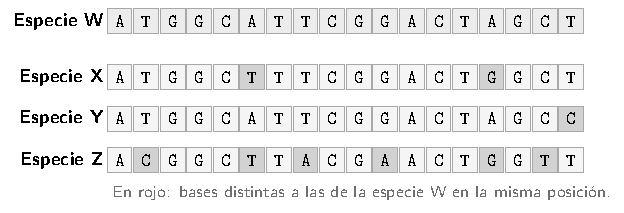
\includegraphics[max width=0.92\linewidth,max height=8.5cm]{bio/evo_secuencias}
\end{center}
 
\begin{ejemplo}[{Ejemplo resuelto}] En la figura, la especie Y difiere de W en 1 base, X en 2 y Z en 6. De mayor a menor parentesco con W: \textbf{Y, X, Z}.\end{ejemplo}
\subsection{Registro fósil}
Un \textbf{fósil} es un resto (huesos, conchas, dientes) o una huella de un organismo del pasado conservado en las rocas. La mayoría se forma en \textbf{rocas sedimentarias}, que se depositan en capas o \textbf{estratos}.

 

\textbf{Datación relativa.} Si los estratos no han sido alterados, los de abajo se depositaron primero: son \textbf{más antiguos} (principio de superposición). Así se ordenan los fósiles del más antiguo al más reciente, sin saber su edad en años.

 

\textbf{Datación absoluta.} Mide la edad en años usando isótopos radiactivos de las rocas o de los restos, como el carbono-14 para restos de hasta unos 50 000 años.

 

\textbf{Fósiles de transición.} Tienen rasgos de dos grupos. \emph{Archaeopteryx} (unos 150 millones de años) tenía plumas y alas como un ave, y dientes, garras en las alas y una cola larga con huesos como un reptil. \emph{Tiktaalik} (unos 375 millones de años) era un pez con cuello móvil y aletas con huesos similares a los de un brazo.

  
\begin{center}
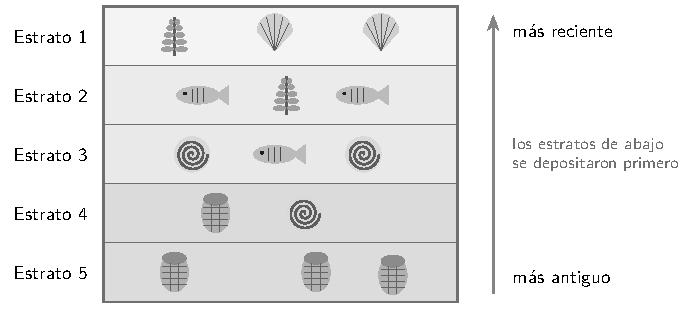
\includegraphics[max width=0.92\linewidth,max height=8.5cm]{bio/evo_estratos}
\end{center}
 
\begin{clave}[{Qué responde y qué no}] Con una columna de estratos se puede responder \textbf{qué especie es más antigua} y \textbf{cuáles vivieron en la misma época} (aparecen en el mismo estrato). No basta para saber la causa de una extinción ni quién desciende de quién.\end{clave}
\subsection{Árboles filogenéticos}
Un \textbf{árbol filogenético} resume las relaciones de parentesco que se deducen de todas las evidencias. Se lee así:

 
\begin{itemize}
  \item Las \textbf{puntas} de las ramas son las especies (actuales o extintas).
  \item Cada \textbf{nodo} (punto donde se separan dos ramas) representa un \textbf{ancestro común}.
  \item Dos especies están más emparentadas mientras \textbf{más reciente} sea el nodo que comparten (más cerca de las puntas).
\end{itemize}
 

En el árbol de la figura, el lagarto y el ave comparten un ancestro más reciente que el que comparten el lagarto y el ratón. Por eso el lagarto está más emparentado con el ave que con el ratón, aunque a simple vista se parezca más al ratón (cuatro patas, sin plumas).

  
\begin{center}
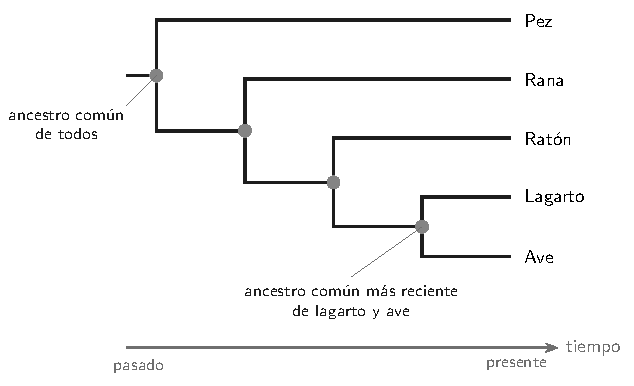
\includegraphics[max width=0.92\linewidth,max height=8.5cm]{bio/evo_arbol}
\end{center}
 
\begin{clave}[{Recuerda}] · Lo que importa son los nodos, no el orden vertical de los nombres: girar las ramas en un nodo no cambia el árbol.\par · Las especies actuales no descienden unas de otras: comparten ancestros. El ser humano y el chimpancé comparten un ancestro común.\end{clave}
\subsection{Lo clave del tema}
\begin{center}\small
\begin{tabularx}{\linewidth}{@{}>{\raggedright\arraybackslash\hsize=0.66\hsize}X>{\raggedright\arraybackslash\hsize=1.06\hsize}X>{\raggedright\arraybackslash\hsize=1.14\hsize}X>{\raggedright\arraybackslash\hsize=1.14\hsize}X@{}}
\toprule
\textbf{Evidencia} & \textbf{Qué se compara} & \textbf{Qué indica} & \textbf{Ejemplo} \\
\midrule
Estructuras homólogas & mismo origen y plan, distinta función & ancestro común (divergencia) & brazo, aleta de ballena, ala de murciélago \\
Estructuras análogas & misma función, distinto origen & convergencia, no parentesco cercano & ala de mariposa y ala de ave \\
Estructuras vestigiales & estructuras reducidas & ancestros con la estructura desarrollada & pelvis de ballena, cóccix \\
Embriología & etapas tempranas del desarrollo & ancestro común & arcos faríngeos y cola en vertebrados \\
Biología molecular & secuencias de ADN o de aminoácidos & menos diferencias = parentesco más cercano & citocromo c \\
Registro fósil & fósiles en estratos & orden de aparición, formas de transición & \emph{Archaeopteryx}, \emph{Tiktaalik} \\
\bottomrule
\end{tabularx}
\end{center}
 
\begin{clave}[{Recuerda}] · Solo las estructuras homólogas indican parentesco; las análogas indican ambientes parecidos.\par · En estratos no alterados, más abajo es más antiguo.\par · Una tabla de diferencias o de similitud indica parentesco, no qué especie apareció primero.\par · En un árbol, el parentesco lo da el nodo compartido más reciente.\end{clave}
 
\begin{clave}[{Método PAES}] 1. Identifica la evidencia (anatomía, embrión, secuencia, fósil). 2. Pregúntate qué permite concluir esa evidencia y qué no (parentesco, orden de antigüedad, causa). 3. En tablas, busca la menor diferencia o la mayor similitud. 4. En árboles, busca el nodo más reciente que une a las especies. 5. Descarta las alternativas que van más allá de los datos.\end{clave}
\begin{elejemplo}{PAES Regular 2026, adaptada}
Un equipo de investigación secuenció el mismo fragmento de un gen en cuatro especies de anfibios, W, X, Y y Z. La figura muestra las secuencias alineadas; en rojo están las bases que difieren de las de la especie W en la misma posición.

A partir de estos datos, ¿cuál de las siguientes opciones ordena las especies X, Y y Z de \textbf{mayor a menor} parentesco con la especie W?
\begin{center}
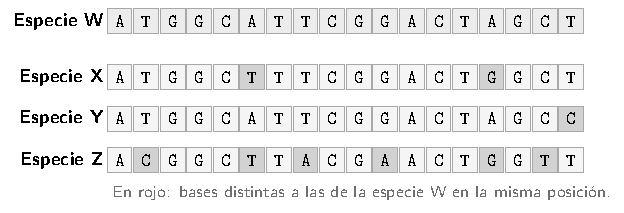
\includegraphics[max width=0.92\linewidth,max height=8.5cm]{bio/evo_secuencias}
\end{center}
\alts{X, Y, Z}{Z, X, Y}{Y, X, Z}{Y, Z, X}
\solucion{\textbf{Paso 1. ¿Qué nos piden?} Ordenar las especies según su parentesco con W, usando la comparación de secuencias de ADN.

\textbf{Paso 2. Cuenta las diferencias.} Recorre cada secuencia y cuenta las bases marcadas: X tiene 2 (posiciones 6 y 15), Y tiene 1 (posición 18) y Z tiene 6.

\textbf{Paso 3. Aplica la regla.} Las diferencias se acumulan con el tiempo desde que dos linajes se separaron. Menos diferencias significa un ancestro común más reciente, es decir, un parentesco más cercano.

\textbf{Respuesta:} Y (1 diferencia), X (2) y Z (6).

\textbf{¿Por qué no las otras?} «X, Y, Z» pone primero a X, que tiene más diferencias que Y. «Z, X, Y» invierte la regla: ordena de menor a mayor parentesco. «Y, Z, X» pone a Z antes que X, aunque Z tiene 6 diferencias y X solo 2.

\textbf{\color{cienciaD}Para recordar.} Menos diferencias en la secuencia = ancestro común más reciente = parentesco más cercano.}{C}
\end{elejemplo}
\motivacion{Fósiles, órganos homólogos y ADN: las evidencias se van sumando. Tus horas de estudio también.}

%% =====================================================================
%% bio_seleccion
\section[Darwin, Wallace y la selección natural]{Darwin, Wallace y la selección natural}
\modcomun\ \ {\color{gris}\itshape Los aportes de Darwin y Wallace, los fundamentos de la selección natural y sus ejemplos (polilla moteada, resistencia a antibióticos y pesticidas, pinzones), y la lectura de gráficos de frecuencia a lo largo de generaciones.\par}
\subsection{Darwin y Wallace}
\textbf{Charles Darwin} viajó alrededor del mundo en el barco \emph{Beagle} (1831-1836), con largas estadías en Sudamérica, incluido Chile, y una visita a las islas Galápagos. Allí notó que especies muy parecidas, como los pinzones y las tortugas, variaban de una isla a otra.

 

Al volver, reunió más evidencias: la \textbf{selección artificial} que hacen los criadores de palomas y ganado, y las ideas de Malthus sobre poblaciones que crecen más rápido que sus recursos.

 

\textbf{Alfred Russel Wallace}, estudiando la fauna del Amazonas y del archipiélago malayo, llegó por su cuenta a la misma explicación. En 1858 le envió a Darwin un ensayo con la idea, y ese mismo año se presentaron juntos los trabajos de ambos en la Sociedad Linneana de Londres.

 

En 1859 Darwin publicó \emph{El origen de las especies}, con abundantes evidencias de la \textbf{evolución por selección natural}.

  
\begin{clave}[{Qué aportó cada uno}] · \textbf{Darwin:} la teoría de la descendencia con modificación y de la selección natural, sostenida con una enorme cantidad de evidencias.\par · \textbf{Wallace:} llegó de forma independiente a la selección natural y estudió la distribución geográfica de las especies (biogeografía).\end{clave}
 
\begin{clave}[{Recuerda}] Darwin y Wallace no conocían los genes. Durante el siglo XX, la genética explicó el origen de la variación (mutaciones y recombinación) y se unió a la selección natural en la \textbf{teoría sintética} de la evolución.\end{clave}
\subsection{Fundamentos de la selección natural}
La selección natural se apoya en cuatro hechos observables:

 
\begin{enumerate}
  \item \textbf{Variación heredable.} Los individuos de una población difieren en sus características, y parte de esas diferencias se heredan.
  \item \textbf{Sobreproducción.} Nacen más individuos de los que el ambiente puede sostener.
  \item \textbf{Lucha por la existencia.} Los recursos son limitados: los individuos compiten por alimento, espacio o pareja, y enfrentan depredadores y enfermedades.
  \item \textbf{Supervivencia y reproducción diferencial.} Los individuos con características más favorables en ese ambiente sobreviven y dejan \textbf{más descendencia}.
\end{enumerate}
 

\textbf{Resultado:} a lo largo de generaciones aumenta en la población la frecuencia de las características favorables. Así se forman las \textbf{adaptaciones}.

  
\begin{clave}[{Adaptación}] Característica heredable que aumenta la supervivencia o la reproducción de un individuo en un ambiente determinado. Lo que cuenta es el \textbf{éxito reproductivo}: un rasgo que atrae más parejas también es adaptativo.\end{clave}
 
\begin{clave}[{Recuerda}] · La variación existe \textbf{antes} del cambio ambiental; surge al azar por mutaciones y recombinación.\par · El ambiente \textbf{selecciona} entre variantes que ya existen.\par · La selección actúa sobre individuos, y lo que cambia es la frecuencia de las características en la \textbf{población}.\end{clave}
\subsection{Ejemplos: polilla moteada y pinzones}
\textbf{Polilla moteada} (\emph{Biston betularia}). En Inglaterra hay polillas claras y oscuras; el color es heredable. Antes de la Revolución Industrial, los troncos estaban cubiertos de líquenes claros y casi todas las polillas eran claras. El hollín de las fábricas oscureció los troncos: las polillas oscuras quedaron mejor camufladas frente a las aves que las cazan, sobrevivieron y se reprodujeron más, y llegaron a ser la gran mayoría. Cuando las leyes redujeron la contaminación, los troncos se aclararon y la tendencia se invirtió.

 

\textbf{Pinzones de Galápagos.} Las distintas especies descienden de un ancestro que llegó desde el continente; sus picos se diversificaron según el alimento de cada ambiente. Peter y Rosemary Grant lo midieron en la isla Daphne Mayor: tras la sequía de 1977 quedaron sobre todo semillas grandes y duras, sobrevivieron más los pinzones de pico más grande y profundo, y la generación siguiente tuvo, en promedio, picos más profundos.

  
\begin{center}
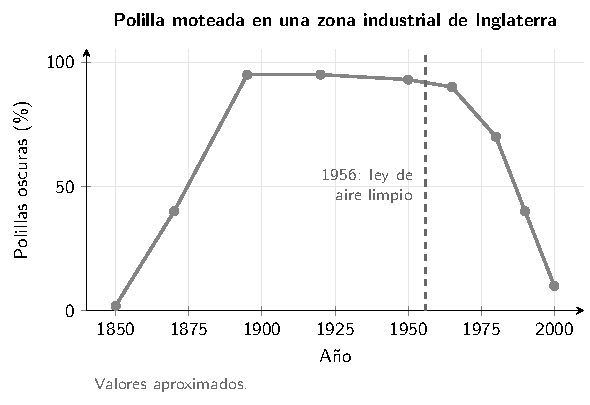
\includegraphics[max width=0.92\linewidth,max height=8.5cm]{bio/evo_polilla}
\end{center}
 
\begin{clave}[{Cómo leer un gráfico de frecuencias}] 1. Mira qué característica se mide y en qué unidad (\% de la población). 2. Ubica cuándo cambia el ambiente. 3. Describe la tendencia después del cambio: si una variante aumenta generación tras generación, el ambiente la está favoreciendo.\end{clave}
\subsection{Ejemplos: resistencia a antibióticos y pesticidas}
En una población de bacterias hay variación: por \textbf{mutaciones al azar}, o por genes recibidos de otras bacterias, algunas pocas son resistentes a un antibiótico antes de que se use.

 
\begin{enumerate}
  \item Al aplicar el antibiótico, mueren las bacterias sensibles. El antibiótico actúa como \textbf{presión de selección}.
  \item Las resistentes sobreviven y se reproducen, con poca competencia.
  \item Tras varias generaciones, casi toda la población es resistente.
\end{enumerate}
 

Lo mismo ocurre con los \textbf{insectos y los pesticidas}, y con las malezas y los herbicidas: el producto elimina a los sensibles y deja a los que ya eran resistentes.

 

Por eso los antibióticos se usan solo con receta, nunca contra virus (como el resfrío), y el tratamiento se cumple completo, como lo indique el médico.

  
\begin{center}
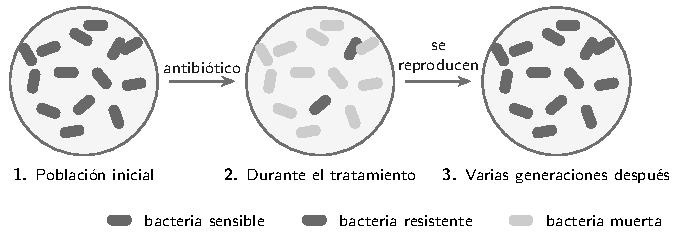
\includegraphics[max width=0.92\linewidth,max height=8.5cm]{bio/evo_bacterias}
\end{center}
 
\begin{clave}[{Recuerda}] El antibiótico no crea la resistencia: selecciona a las bacterias que ya la tenían. La población cambia porque cambia la proporción de bacterias resistentes.\end{clave}
\subsection{Lo clave del tema}
\begin{center}\small
\begin{tabularx}{\linewidth}{@{}>{\raggedright\arraybackslash\hsize=0.79\hsize}X>{\raggedright\arraybackslash\hsize=1.13\hsize}X>{\raggedright\arraybackslash\hsize=1.08\hsize}X@{}}
\toprule
\textbf{Concepto} & \textbf{Idea central} & \textbf{Ejemplo} \\
\midrule
Darwin y Wallace (1858-1859) & evolución por selección natural & pinzones, selección artificial \\
Variación heredable & existe antes del cambio ambiental & polillas claras y oscuras \\
Presión de selección & factor del ambiente que favorece a unas variantes & antibiótico, depredador, sequía \\
Reproducción diferencial & los mejor adaptados dejan más descendencia & pinzones de pico profundo en la sequía \\
Adaptación & rasgo heredable que aumenta la supervivencia o la reproducción & camuflaje, resistencia \\
\bottomrule
\end{tabularx}
\end{center}
 
\begin{clave}[{Recuerda}] · Los caracteres adquiridos durante la vida no se heredan.\par · La variación surge al azar; el ambiente selecciona.\par · Evoluciona la población, no el individuo.\par · Ser adaptativo significa dejar más descendencia en ese ambiente.\end{clave}
 
\begin{clave}[{Método PAES}] 1. Busca la variación previa en la población. 2. Identifica la presión de selección (qué cambió en el ambiente). 3. Pregunta qué variante sobrevive y se reproduce más. 4. Predice: esa variante aumenta su frecuencia a lo largo de generaciones. 5. Descarta las alternativas que dicen «para», «porque lo necesitaban» o «lo adquirieron y lo heredaron».\end{clave}
\begin{elejemplo}{Estilo PAES}
En una isla vive una especie de ave que se alimenta de semillas; la profundidad del pico es una característica heredable. Durante una sequía de dos años, las plantas de semillas pequeñas y blandas casi desaparecieron, y quedaron sobre todo semillas grandes y duras, que solo las aves de pico profundo logran romper. El gráfico muestra la profundidad del pico en la población antes de la sequía y en la generación nacida después.

¿Qué explicación del cambio es coherente con la selección natural?
\begin{center}
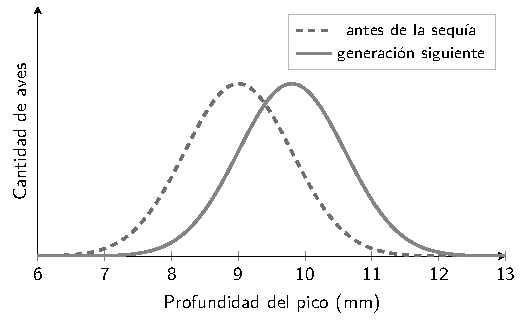
\includegraphics[max width=0.92\linewidth,max height=8.5cm]{bio/evo_pinzones}
\end{center}
\altslargas{Al romper semillas duras, cada ave fortaleció y agrandó su pico, y heredó ese cambio a sus crías.}{Las aves de pico más profundo sobrevivieron y se reprodujeron más durante la sequía, y sus crías heredaron esa característica.}{La sequía causó mutaciones que hicieron crecer el pico de todas las aves de la isla.}{Las aves necesitaban picos más grandes, por lo que sus crías nacieron con picos más profundos.}
\solucion{\textbf{Paso 1. ¿Qué nos piden?} Explicar con la selección natural por qué la curva se desplazó hacia picos más profundos.

\textbf{Paso 2. Variación previa.} Antes de la sequía ya había aves con picos de distintas profundidades: la curva gris va de unos 7 a unos 11 mm.

\textbf{Paso 3. Presión de selección.} La sequía dejó solo semillas grandes y duras. Las aves de pico profundo podían comerlas: sobrevivieron y se reprodujeron más que las de pico poco profundo.

\textbf{Paso 4. Herencia.} Como la profundidad del pico es heredable, la generación siguiente tuvo más aves de pico profundo: la curva naranja está corrida hacia la derecha.

\textbf{Respuesta:} las aves de pico más profundo sobrevivieron y se reprodujeron más, y sus crías heredaron esa característica.

\textbf{¿Por qué no las otras?} Que el pico de cada ave cambie por el uso no explica nada: un cambio adquirido durante la vida no modifica el ADN de los gametos y no se transmite. Las mutaciones ocurren al azar, no son causadas por la necesidad ni afectan a toda la población a la vez. «Necesitaban picos más grandes» tampoco sirve: la necesidad no produce la variación.

\textbf{\color{cienciaD}Para recordar.} El ambiente no cambia a los individuos: favorece a las variantes que ya existían, y la población cambia.}{B}
\end{elejemplo}
\motivacion{Sobreviven los que mejor se adaptan, y tú te estás adaptando a la PAES tema por tema.}

\chapter{Organismo y ambiente}
%% =====================================================================
%% bio_fotosintesis
\section[Fotosíntesis]{Fotosíntesis}
\modcomun\ \ {\color{gris}\itshape Qué es la fotosíntesis y su ecuación global, el efecto de la luz, el CO\textsubscript{2} y la temperatura (factor limitante), y los experimentos clásicos con Elodea, agua marcada y lugol.\par}
\subsection{Qué es la fotosíntesis}
La \textbf{fotosíntesis} es el proceso en que los organismos \textbf{autótrofos fotosintéticos} (plantas, algas y cianobacterias) usan la \textbf{energía de la luz} para fabricar materia orgánica (glucosa) a partir de materia inorgánica: \textbf{dióxido de carbono} y \textbf{agua}.

 

Su ecuación global es:

 
\begin{center}
\textbf{6 CO\textsubscript{2} + 6 H\textsubscript{2}O \ensuremath{\rightarrow} C\textsubscript{6}H\textsubscript{12}O\textsubscript{6} + 6 O\textsubscript{2}}\par \textcolor{gris}{(con luz y clorofila)}
\end{center}
 
\begin{itemize}
  \item \textbf{Reactantes:} CO\textsubscript{2} (entra a la hoja por los estomas) y H\textsubscript{2}O (sube desde las raíces).
  \item \textbf{Productos:} glucosa, que la planta usa como combustible o guarda como \textbf{almidón}, y O\textsubscript{2}, que se libera al ambiente.
  \item \textbf{Transformación de energía:} la energía luminosa queda guardada como \textbf{energía química} en los enlaces de la glucosa.
\end{itemize}
  
\begin{clave}[{Por qué importa}] Casi toda la energía que circula por los ecosistemas entró por la fotosíntesis. Además, es la principal fuente del O\textsubscript{2} de la atmósfera y saca CO\textsubscript{2} del aire: es la puerta de entrada del carbono a los seres vivos.\end{clave}
 
\begin{clave}[{Recuerda}] En plantas y algas la fotosíntesis ocurre en los \textbf{cloroplastos}, organelos que abundan en las células de las hojas y contienen la \textbf{clorofila}, el pigmento que capta la luz. El O\textsubscript{2} liberado viene del \textbf{agua}; el carbono de la glucosa, del \textbf{CO\textsubscript{2}}.\end{clave}
\subsection{Factores que afectan la tasa fotosintética}
\begin{center}
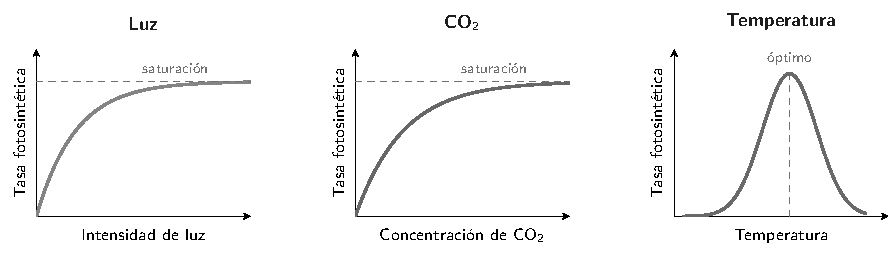
\includegraphics[max width=0.92\linewidth,max height=8.5cm]{bio/amb_factores}
\end{center}
  
\begin{itemize}
  \item \textbf{Intensidad de luz:} al aumentarla, sube la tasa, hasta un punto de \textbf{saturación} en que más luz ya no aumenta la tasa.
  \item \textbf{Concentración de CO\textsubscript{2}:} igual que la luz, sube y se satura.
  \item \textbf{Temperatura:} las enzimas de la fotosíntesis tienen una temperatura \textbf{óptima}. Bajo ella trabajan lento; muy por sobre ella se desnaturalizan y la tasa cae a cero.
\end{itemize}
  
\begin{clave}[{Factor limitante}] Es el factor que está en menor cantidad respecto de lo que se necesita: él fija la tasa, aunque los demás sobren. En la parte que sube de la curva de luz, el limitante es la luz. En la meseta, el limitante es otro factor (CO\textsubscript{2} o temperatura): si se aumenta ese otro factor, la meseta sube.\end{clave}
\subsection{Experimentos clásicos}
\textbf{Elodea y burbujas de O\textsubscript{2}.} Se pone una planta acuática (Elodea) en agua con bicarbonato (fuente de CO\textsubscript{2}) y se ilumina con una lámpara a distintas distancias. Se cuentan las burbujas de O\textsubscript{2} por minuto: a menor distancia (más luz), más burbujas. La distancia de la lámpara es la \textbf{variable independiente}; las burbujas por minuto, la \textbf{dependiente}; la temperatura y el bicarbonato se mantienen \textbf{constantes}.

 

\textbf{Origen del O\textsubscript{2} (agua marcada).} Se usa oxígeno pesado (\textsuperscript{18}O) como marcador. Si se marca el agua, el O\textsubscript{2} liberado sale marcado; si se marca el CO\textsubscript{2}, no. Conclusión: el O\textsubscript{2} de la fotosíntesis viene del \textbf{agua}.

 

\textbf{Almidón y lugol.} El lugol tiñe de azul oscuro el almidón. En una hoja con zonas blancas (sin clorofila), solo las zonas verdes se tiñen: sin clorofila no hay fotosíntesis.

  
\begin{center}
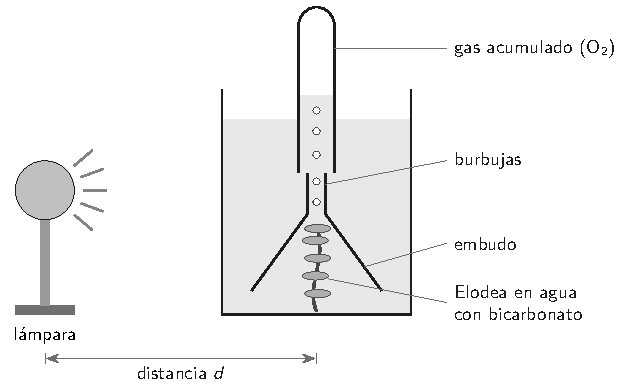
\includegraphics[max width=0.92\linewidth,max height=8.5cm]{bio/amb_elodea}
\end{center}
 
\begin{center}
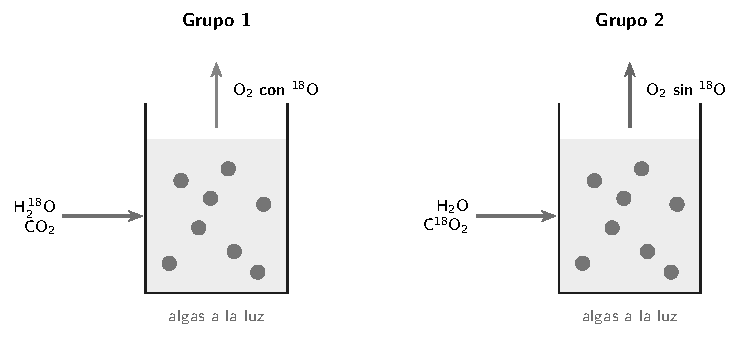
\includegraphics[max width=0.92\linewidth,max height=8.5cm]{bio/amb_isotopos}
\end{center}
\subsection{Lo clave del tema}
\begin{center}\small
\begin{tabularx}{\linewidth}{@{}>{\raggedright\arraybackslash\hsize=0.67\hsize}X>{\raggedright\arraybackslash\hsize=1.33\hsize}X@{}}
\toprule
\textbf{Factor} & \textbf{Efecto sobre la tasa fotosintética} \\
\midrule
Intensidad de luz & sube hasta una saturación \\
Concentración de CO\textsubscript{2} & sube hasta una saturación \\
Temperatura & máxima en el óptimo; baja a ambos lados y se detiene si las enzimas se desnaturalizan \\
\bottomrule
\end{tabularx}
\end{center}
 
\begin{clave}[{Recuerda}] · 6 CO\textsubscript{2} + 6 H\textsubscript{2}O \ensuremath{\rightarrow} C\textsubscript{6}H\textsubscript{12}O\textsubscript{6} + 6 O\textsubscript{2}, con luz y clorofila.\par · El O\textsubscript{2} liberado viene del agua; el carbono de la glucosa, del CO\textsubscript{2}.\par · La glucosa se usa como combustible o se guarda como almidón, que se detecta con lugol.\par · Luz y CO\textsubscript{2} aumentan la tasa hasta una saturación; la temperatura tiene un óptimo.\par · El factor limitante es el que fija la tasa; al aumentarlo, la tasa sube.\end{clave}
 
\begin{clave}[{Método PAES}] 1. Identifica qué mide el experimento (O\textsubscript{2} liberado, CO\textsubscript{2} captado, glucosa o almidón): todos indican cuánta fotosíntesis hubo. 2. Separa la variable independiente (la que se cambia), la dependiente (la que se mide) y las controladas. 3. En un gráfico, busca dónde la curva sube (ese factor limita) y dónde se aplana (limita otro). 4. Revisa cada alternativa contra los datos: no aceptes conclusiones que el experimento no midió.\end{clave}
\begin{elejemplo}{PAES Regular 2026, adaptada}
Un grupo de estudiantes mide la producción de O\textsubscript{2} de una planta acuática a distintas intensidades de luz, con dos concentraciones de CO\textsubscript{2} en el agua y siempre a 25 °C. Sus resultados se muestran en el gráfico:

Con una intensidad de luz de 8 u.a. y CO\textsubscript{2} al 0,03 \%, ¿qué factor limita la producción de O\textsubscript{2}?
\begin{center}
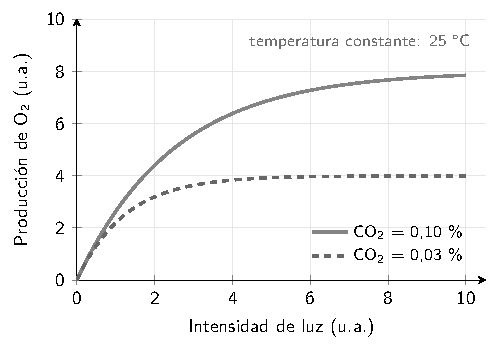
\includegraphics[max width=0.92\linewidth,max height=8.5cm]{bio/amb_limitante}
\end{center}
\alts{La intensidad de luz.}{La concentración de CO\textsubscript{2}.}{La temperatura.}{La cantidad de agua disponible.}
\solucion{\textbf{Paso 1. ¿Qué nos piden?} El factor limitante en un punto del gráfico: el que, si se aumenta, hace subir la producción de O\textsubscript{2}.

\textbf{Paso 2. Mira la curva de CO\textsubscript{2} al 0,03 \%.} Desde una intensidad de 4 u.a. la curva está plana: al pasar de 4 a 8 u.a. de luz la producción se queda en 4 u.a. Más luz no cambia nada, así que la luz ya no limita.

\textbf{Paso 3. Compara con la otra curva.} Con la misma luz (8 u.a.) y la misma temperatura, pero con CO\textsubscript{2} al 0,10 \%, la producción sube a casi 8 u.a. El único factor que cambió fue el CO\textsubscript{2}, y al aumentarlo la producción subió.

\textbf{Respuesta:} la concentración de CO\textsubscript{2} limita la producción en ese punto.

\textbf{¿Por qué no las otras?} La intensidad de luz limita solo en la parte de la curva que sube (bajo 3 u.a. aproximadamente). La temperatura fue la misma, 25 °C, en ambas curvas, así que no explica la diferencia. El agua no fue una variable del experimento: la planta está sumergida.

\textbf{\color{cienciaD}Para recordar.} En la meseta la luz ya no limita: limita el factor que, al aumentarlo, eleva la meseta.}{B}
\end{elejemplo}
\motivacion{Una planta convierte la luz en energía química. Convierte tú este esfuerzo en puntaje.}

%% =====================================================================
%% bio_respiracion
\section[Respiración celular y nutrición]{Respiración celular y nutrición}
\modcomun\ \ {\color{gris}\itshape Nutrición autótrofa y heterótrofa, la respiración celular en la mitocondria (reactantes, productos, ATP y ecuación global), la relación complementaria entre fotosíntesis y respiración y los experimentos con azul de bromotimol y semillas en germinación.\par}
\subsection{Nutrición autótrofa y heterótrofa}
Todo ser vivo necesita materia orgánica: como fuente de \textbf{energía} y como material para \textbf{construir} su cuerpo. Según cómo la obtiene, su nutrición es de dos tipos.

 
\begin{itemize}
  \item \textbf{Autótrofa:} el organismo fabrica su propia materia orgánica a partir de materia inorgánica (CO\textsubscript{2}, agua, sales).\par · \textbf{Fotosintéticos:} usan la energía de la luz (plantas, algas, cianobacterias).\par · \textbf{Quimiosintéticos:} usan la energía de reacciones químicas con sustancias inorgánicas (algunas bacterias de fuentes hidrotermales o del suelo).
  \item \textbf{Heterótrofa:} el organismo obtiene la materia orgánica de otros seres vivos o de sus restos: animales, hongos, la mayoría de las bacterias y muchos protozoos.
\end{itemize}
  
\begin{center}\small
\begin{tabularx}{\linewidth}{@{}>{\raggedright\arraybackslash\hsize=0.78\hsize}X>{\raggedright\arraybackslash\hsize=0.97\hsize}X>{\raggedright\arraybackslash\hsize=1.25\hsize}X@{}}
\toprule
 & \textbf{Autótrofos} & \textbf{Heterótrofos} \\
\midrule
Fuente de carbono & CO\textsubscript{2} & materia orgánica de otros \\
Fuente de energía & luz o reacciones químicas & la materia orgánica que consumen \\
Rol en el ecosistema & productores & consumidores y descomponedores \\
¿Respiran? & sí & sí \\
\bottomrule
\end{tabularx}
\end{center}
 
\begin{clave}[{Recuerda}] Las plantas también respiran, de día y de noche, en todas sus células vivas: la fotosíntesis fabrica la glucosa y la respiración celular la usa para obtener ATP.\end{clave}
\subsection{La respiración celular}
La \textbf{respiración celular aeróbica} degrada la glucosa usando O\textsubscript{2} y guarda parte de su energía en moléculas de \textbf{ATP}, la "moneda energética" de la célula. Ocurre en las células de casi todos los seres vivos, autótrofos y heterótrofos.

 
\begin{center}
\textbf{C\textsubscript{6}H\textsubscript{12}O\textsubscript{6} + 6 O\textsubscript{2} \ensuremath{\rightarrow} 6 CO\textsubscript{2} + 6 H\textsubscript{2}O + energía (ATP y calor)}
\end{center}
 
\begin{itemize}
  \item \textbf{Reactantes:} glucosa y O\textsubscript{2}.
  \item \textbf{Productos:} CO\textsubscript{2}, H\textsubscript{2}O y energía. Parte queda en el ATP (unas 30 a 32 moléculas por glucosa) y el resto se libera como \textbf{calor}.
  \item \textbf{Lugar:} comienza en el citoplasma (glucólisis) y se completa en la \textbf{mitocondria}.
\end{itemize}
  
\begin{center}
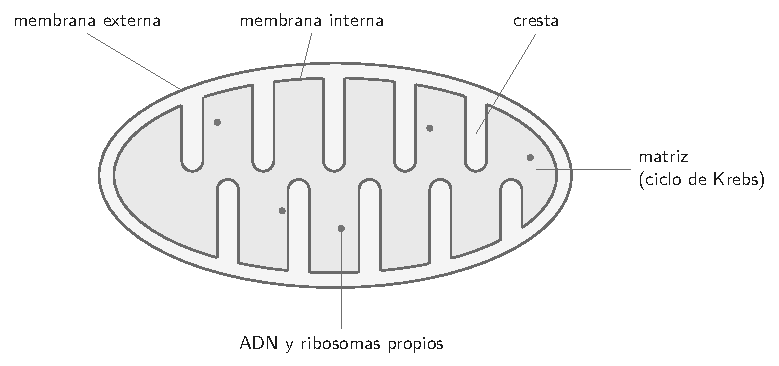
\includegraphics[max width=0.92\linewidth,max height=8.5cm]{bio/amb_mitocondria}
\end{center}
 
\begin{clave}[{Recuerda}] Es un proceso \textbf{catabólico}: rompe una molécula grande (glucosa) en moléculas pequeñas (CO\textsubscript{2} y H\textsubscript{2}O) y libera energía.\end{clave}
\subsection{Las etapas, en resumen}
\begin{center}\small
\begin{tabularx}{\linewidth}{@{}>{\raggedright\arraybackslash\hsize=1.11\hsize}X>{\raggedright\arraybackslash\hsize=0.74\hsize}X>{\raggedright\arraybackslash\hsize=1.14\hsize}X@{}}
\toprule
\textbf{Etapa} & \textbf{Lugar} & \textbf{Qué pasa} \\
\midrule
Glucólisis & citoplasma & la glucosa se divide en dos moléculas de piruvato; se forman 2 ATP \\
Ciclo de Krebs & matriz mitocondrial & el piruvato se oxida por completo; se libera \textbf{CO\textsubscript{2}} \\
Cadena transportadora y síntesis de ATP & membrana interna (crestas) & el \textbf{O\textsubscript{2}} recibe los electrones y forma \textbf{H\textsubscript{2}O}; se produce la mayor parte del ATP \\
\bottomrule
\end{tabularx}
\end{center}
  
\begin{clave}[{¿De dónde viene y a dónde va cada cosa?}] · El CO\textsubscript{2} que exhalas se forma en la \textbf{matriz} (ciclo de Krebs).\par · El O\textsubscript{2} que inhalas se usa al final, en las \textbf{crestas}, y termina formando agua.\end{clave}
 
\begin{clave}[{Sin oxígeno}] Algunas células, como las levaduras o las musculares en ejercicio intenso, pueden obtener energía sin O\textsubscript{2} por \textbf{fermentación}. Rinde solo 2 ATP por glucosa, mucho menos que la respiración aeróbica.\end{clave}
\subsection{Fotosíntesis y respiración: procesos complementarios}
\begin{center}
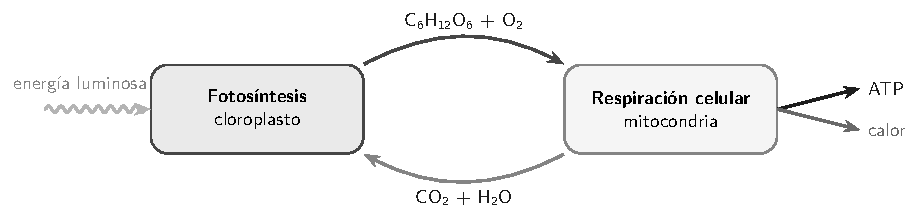
\includegraphics[max width=0.92\linewidth,max height=8.5cm]{bio/amb_complemento}
\end{center}
 
\begin{center}\small
\begin{tabularx}{\linewidth}{@{}>{\raggedright\arraybackslash\hsize=0.42\hsize}X>{\raggedright\arraybackslash\hsize=1.29\hsize}X>{\raggedright\arraybackslash\hsize=1.29\hsize}X@{}}
\toprule
 & \textbf{Fotosíntesis} & \textbf{Respiración celular} \\
\midrule
Organelo & cloroplasto & mitocondria (y citoplasma) \\
Organismos & autótrofos fotosintéticos & autótrofos y heterótrofos \\
Reactantes & CO\textsubscript{2} y H\textsubscript{2}O (más luz) & glucosa y O\textsubscript{2} \\
Productos & glucosa y O\textsubscript{2} & CO\textsubscript{2}, H\textsubscript{2}O y ATP \\
Energía & la luz queda guardada como energía química & la energía química se libera como ATP y calor \\
Cuándo & solo con luz & siempre, de día y de noche \\
\bottomrule
\end{tabularx}
\end{center}
 
\begin{clave}[{La idea clave}] Los productos de una son los reactantes de la otra. La materia (C, H, O) circula entre ambos procesos; la energía no: entra como luz y sale como calor.\end{clave}
\subsection{Experimentos con indicadores}
El \textbf{azul de bromotimol} es un indicador de pH. El CO\textsubscript{2} disuelto en agua forma ácido carbónico y baja el pH.

 
\begin{itemize}
  \item \textbf{Azul:} poco CO\textsubscript{2} (se consumió CO\textsubscript{2}).
  \item \textbf{Verde:} nivel intermedio.
  \item \textbf{Amarillo:} mucho CO\textsubscript{2} (se liberó CO\textsubscript{2}).
\end{itemize}
 

En los tubos de la figura, todos parten verdes. La Elodea a la luz hace más fotosíntesis que respiración y saca CO\textsubscript{2}: el tubo se vuelve azul. En la oscuridad solo respira y el tubo se vuelve amarillo, igual que con el caracol. El tubo sin organismos es el \textbf{control}: muestra que el color no cambia solo.

  
\begin{center}
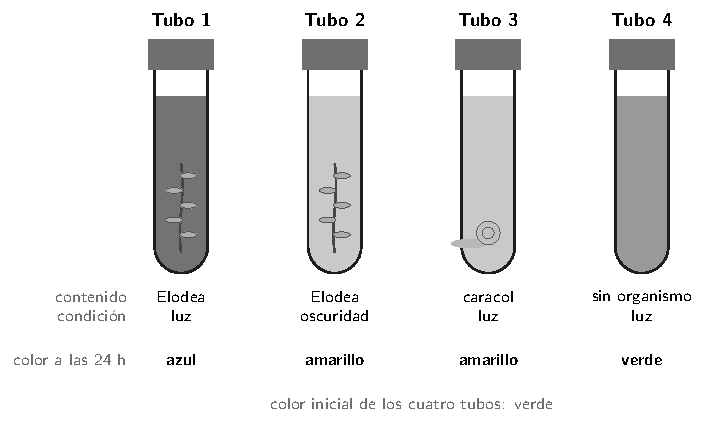
\includegraphics[max width=0.92\linewidth,max height=8.5cm]{bio/amb_tubos_abt}
\end{center}
   

\textbf{Semillas en germinación.} Una semilla que germina respira con mucha intensidad: usa sus reservas, libera CO\textsubscript{2} y desprende calor. Si se comparan con semillas hervidas (muertas), solo en el frasco de las semillas vivas sube la temperatura y el indicador se pone amarillo.

  
\begin{center}
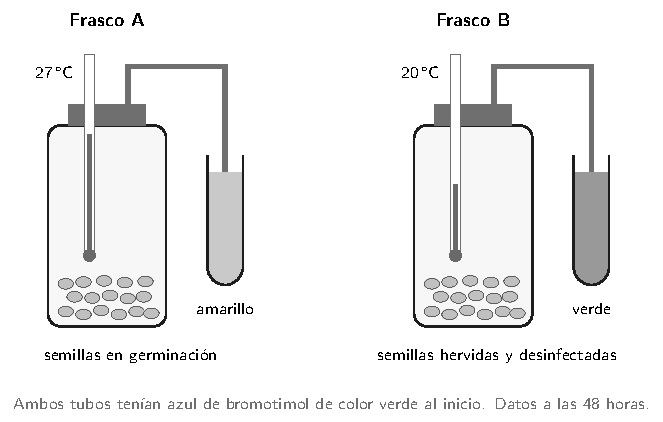
\includegraphics[max width=0.92\linewidth,max height=8.5cm]{bio/amb_semillas}
\end{center}
\subsection{Lo clave del tema}
\begin{center}\small
\begin{tabularx}{\linewidth}{@{}>{\raggedright\arraybackslash\hsize=0.69\hsize}X>{\raggedright\arraybackslash\hsize=1.31\hsize}X@{}}
\toprule
\textbf{Concepto} & \textbf{Idea central} \\
\midrule
Nutrición autótrofa & fabrica materia orgánica desde CO\textsubscript{2} (con luz o energía química) \\
Nutrición heterótrofa & obtiene la materia orgánica de otros seres vivos \\
Respiración celular & glucosa + O\textsubscript{2} \ensuremath{\rightarrow} CO\textsubscript{2} + H\textsubscript{2}O + ATP y calor; en la mitocondria \\
Azul de bromotimol & amarillo = más CO\textsubscript{2}; azul = menos CO\textsubscript{2} \\
\bottomrule
\end{tabularx}
\end{center}
 
\begin{clave}[{Recuerda}] · Autótrofos y heterótrofos respiran; las plantas respiran de día y de noche.\par · El CO\textsubscript{2} de la respiración se forma en la matriz; el O\textsubscript{2} se usa en las crestas y forma agua.\par · Los productos de la fotosíntesis son los reactantes de la respiración, y viceversa.\end{clave}
 
\begin{clave}[{Método PAES}] 1. Anota qué proceso puede ocurrir en cada condición: con luz, fotosíntesis y respiración; sin luz, solo respiración; en animales y semillas, solo respiración. 2. Decide cuál predomina y qué gas se acumula. 3. Traduce a la medición: más CO\textsubscript{2} \ensuremath{\rightarrow} indicador amarillo; menos CO\textsubscript{2} \ensuremath{\rightarrow} azul; más respiración \ensuremath{\rightarrow} más calor. 4. Busca el control: el tubo o frasco que muestra qué pasa sin el factor estudiado.\end{clave}
\begin{elejemplo}{PAES Invierno 2027, adaptada}
Una profesora prepara cuatro tubos con azul de bromotimol, todos de color verde al inicio, y los tapa. El indicador se vuelve amarillo cuando aumenta el CO\textsubscript{2} disuelto y azul cuando disminuye. Después de 24 horas observa los colores que muestra la figura:

¿Cuál conclusión es correcta?
\begin{center}
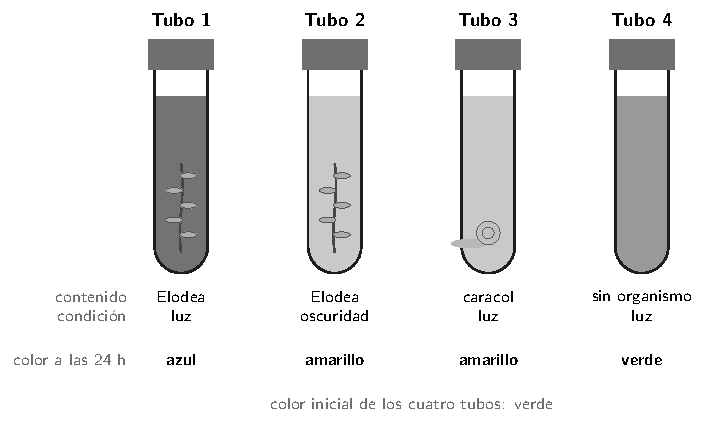
\includegraphics[max width=0.92\linewidth,max height=8.5cm]{bio/amb_tubos_abt}
\end{center}
\altslargas{En el tubo 1, la Elodea consumió más CO\textsubscript{2} del que liberó.}{En el tubo 2, la Elodea hizo fotosíntesis, pero no respiró.}{En el tubo 3, el caracol consumió el CO\textsubscript{2} disuelto.}{El tubo 4 muestra que la luz, por sí sola, vuelve azul el indicador.}
\solucion{\textbf{Paso 1. ¿Qué nos piden?} Interpretar cada color según el CO\textsubscript{2}: azul = bajó, amarillo = subió, verde = no cambió.

\textbf{Paso 2. Tubo 1 (Elodea, luz): azul.} El CO\textsubscript{2} bajó. La planta respira y libera CO\textsubscript{2}, pero a la luz también hace fotosíntesis, que lo consume. Como bajó, consumió más del que liberó.

\textbf{Paso 3. Los demás.} Tubo 2 (oscuridad): amarillo; sin luz no hay fotosíntesis y la respiración liberó CO\textsubscript{2}. Tubo 3: el caracol respira y liberó CO\textsubscript{2}. Tubo 4: sin organismos, el color no cambió.

\textbf{Respuesta:} en el tubo 1, la Elodea consumió más CO\textsubscript{2} del que liberó.

\textbf{¿Por qué no las otras?} En el tubo 2 ocurrió lo contrario: sin luz no hay fotosíntesis, y la planta siguió respirando. El caracol no hace fotosíntesis: libera CO\textsubscript{2} y por eso su tubo se puso amarillo. El tubo 4 recibió luz y quedó verde: la luz sola no cambia el color.

\textbf{\color{cienciaD}Para recordar.} Azul = se consumió CO\textsubscript{2} (fotosíntesis mayor que respiración); amarillo = se liberó CO\textsubscript{2} (respiración).}{A}
\end{elejemplo}
\motivacion{Glucosa y oxígeno: así sacan energía tus células para estudiar. Come bien, respira hondo y sigue.}

%% =====================================================================
%% bio_flujo
\section[Flujo de energía y ciclos del carbono y del oxígeno]{Flujo de energía y ciclos del carbono y del oxígeno}
\modcomun\ \ {\color{gris}\itshape Productores, consumidores y descomponedores; cadenas y tramas tróficas; flujo unidireccional de la energía con pérdida de cerca del 90 \% en cada nivel; pirámides ecológicas; ciclos del carbono y del oxígeno, el rol de la fotosíntesis y la respiración, y el efecto de la combustión y la deforestación.\par}
\subsection{Niveles tróficos}
En un ecosistema, cada organismo ocupa un \textbf{nivel trófico} según cómo obtiene su materia orgánica.

 
\begin{itemize}
  \item \textbf{Productores} (autótrofos): plantas, algas, fitoplancton y cianobacterias. Fabrican materia orgánica por fotosíntesis. Son la puerta de entrada de la energía y del carbono.
  \item \textbf{Consumidores} (heterótrofos): se alimentan de otros seres vivos.\par · \textbf{Primarios} (herbívoros): comen productores.\par · \textbf{Secundarios}: comen consumidores primarios.\par · \textbf{Terciarios}: comen consumidores secundarios.
  \item \textbf{Descomponedores} (hongos y bacterias): degradan restos, desechos y cadáveres de todos los niveles. Devuelven al ambiente el CO\textsubscript{2} y los minerales que los productores vuelven a usar.
\end{itemize}
  
\begin{clave}[{Cadena trófica}] Una secuencia lineal de quién come a quién. Las flechas van desde el alimento hacia quien lo come, porque indican hacia dónde va la energía.\par pasto \ensuremath{\rightarrow} degú \ensuremath{\rightarrow} culebra de cola larga \ensuremath{\rightarrow} águila mora\end{clave}
 
\begin{clave}[{Recuerda}] Un mismo organismo puede ocupar más de un nivel trófico si se alimenta de presas de niveles distintos.\end{clave}
\subsection{Tramas tróficas}
En la naturaleza las cadenas se entrecruzan: casi todos los organismos tienen varias presas y varios depredadores. El conjunto de cadenas conectadas es una \textbf{trama trófica}.

 

En la trama marina de la figura, el lobo marino come jibias y anchovetas: es consumidor \textbf{cuaternario} en una cadena y \textbf{terciario} en otra.

 

\textbf{Para analizar una trama:}

 
\begin{itemize}
  \item Para contar cadenas, parte en cada productor y sigue todas las flechas hasta llegar a un organismo que nadie come.
  \item Si una especie desaparece, sus depredadores pierden alimento (y bajan, salvo que tengan otras presas) y sus presas pierden un depredador (y pueden aumentar).
\end{itemize}
  
\begin{center}
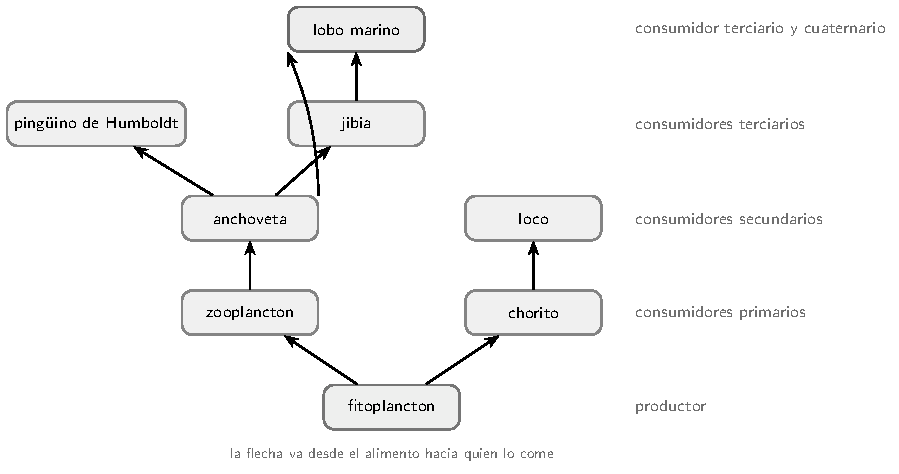
\includegraphics[max width=0.92\linewidth,max height=8.5cm]{bio/amb_trama}
\end{center}
\subsection{El flujo de energía}
\begin{center}
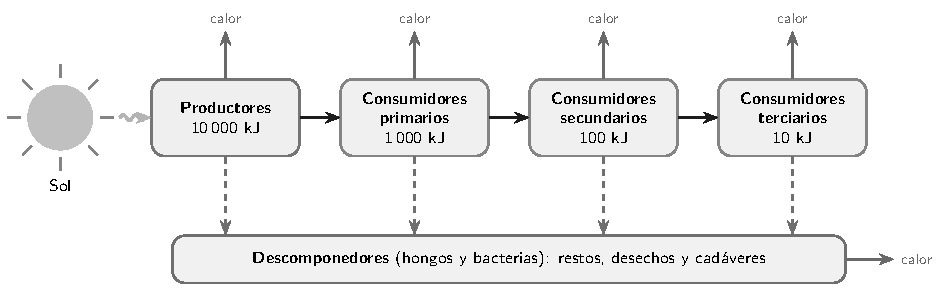
\includegraphics[max width=0.92\linewidth,max height=8.5cm]{bio/amb_flujo_energia}
\end{center}
  
\begin{itemize}
  \item La energía entra como \textbf{luz}, los productores la transforman en \textbf{energía química} y pasa de nivel en nivel con el alimento.
  \item En cada nivel, la mayor parte de la energía se usa en la \textbf{respiración celular} (moverse, mantener la temperatura, crecer) y se pierde como \textbf{calor}. Otra parte no se come o no se digiere y va a los descomponedores.
  \item Solo cerca del \textbf{10 \%} de la energía de un nivel queda en el siguiente.
\end{itemize}
  
\begin{clave}[{Recuerda}] El flujo de energía es \textbf{unidireccional}: el calor no se puede volver a usar para la fotosíntesis. Por eso los ecosistemas necesitan un aporte constante de luz solar. La materia, en cambio, se recicla.\end{clave}
 
\begin{clave}[{Consecuencia}] Las cadenas tróficas son cortas (rara vez más de 4 o 5 niveles): arriba queda muy poca energía.\end{clave}
\subsection{Pirámides ecológicas}
\begin{center}
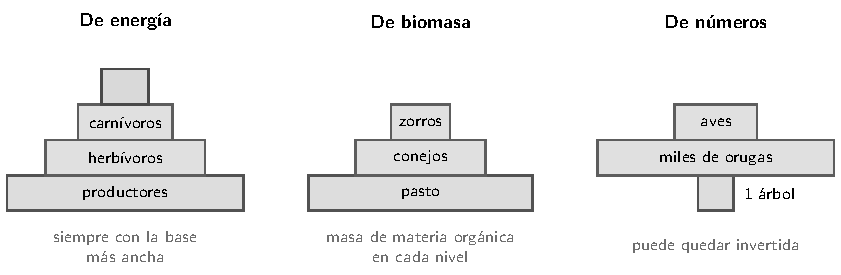
\includegraphics[max width=0.92\linewidth,max height=8.5cm]{bio/amb_piramides}
\end{center}
  
\begin{itemize}
  \item \textbf{De energía:} la energía de cada nivel en un tiempo dado. \textbf{Siempre} tiene la base más ancha, porque en cada paso se pierde energía como calor.
  \item \textbf{De biomasa:} la masa de materia orgánica de cada nivel. Suele tener la base ancha, aunque en algunos ecosistemas acuáticos se invierte (el fitoplancton se reproduce tan rápido que su masa en un momento es menor que la del zooplancton).
  \item \textbf{De números:} la cantidad de individuos. Puede invertirse cuando un productor grande alimenta a muchos consumidores pequeños, como un árbol con miles de orugas.
\end{itemize}
  
\begin{clave}[{Recuerda}] De las tres, solo la pirámide de energía nunca se invierte.\end{clave}
\subsection{El ciclo del carbono}
\begin{center}
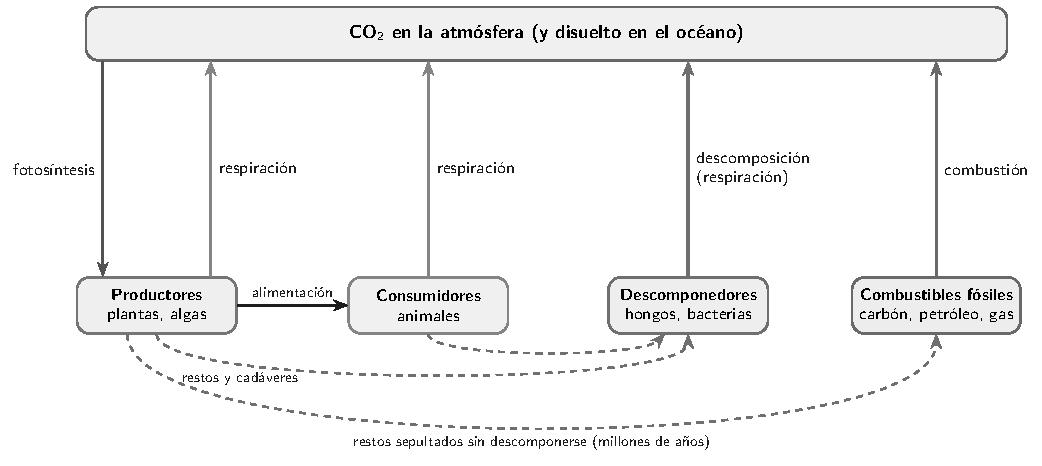
\includegraphics[max width=0.92\linewidth,max height=8.5cm]{bio/amb_ciclo_carbono}
\end{center}
  
\begin{itemize}
  \item \textbf{Entrada a los seres vivos:} la \textbf{fotosíntesis} fija el CO\textsubscript{2} del aire (o disuelto en el agua) en moléculas orgánicas.
  \item \textbf{Paso por la trama:} el carbono pasa a los consumidores con el alimento y a los descomponedores con los restos.
  \item \textbf{Regreso a la atmósfera:} la \textbf{respiración celular} de todos los seres vivos, incluida la de los descomponedores, y la \textbf{combustión}.
  \item \textbf{Reservas lentas:} restos sepultados sin descomponerse, durante millones de años, formaron carbón, petróleo y gas natural.
\end{itemize}
  
\begin{clave}[{Recuerda}] Fotosíntesis y respiración son las dos caras del ciclo: una saca CO\textsubscript{2} de la atmósfera y la otra lo devuelve. A diferencia de la energía, el carbono se recicla una y otra vez.\end{clave}
\subsection{Ciclo del oxígeno y acción humana}
\textbf{Ciclo del oxígeno.} Va unido al del carbono. La \textbf{fotosíntesis} libera O\textsubscript{2} (que viene del agua). La \textbf{respiración celular} y la \textbf{combustión} consumen O\textsubscript{2} y forman CO\textsubscript{2} y agua. Ese CO\textsubscript{2} y esa agua vuelven a usarse en la fotosíntesis.

 

\textbf{Combustión de combustibles fósiles.} Libera en pocos años carbono que estuvo guardado millones de años: aumenta el CO\textsubscript{2} de la atmósfera.

 

\textbf{Deforestación.} Aumenta el CO\textsubscript{2} por dos vías: si el bosque se quema, su carbono pasa al aire como CO\textsubscript{2}; y sin los árboles, se fija menos CO\textsubscript{2} por fotosíntesis.

 

El CO\textsubscript{2} es un gas de efecto invernadero: su aumento intensifica el calentamiento global.

  
\begin{center}
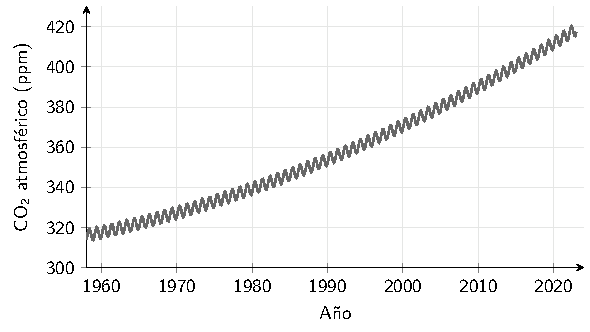
\includegraphics[max width=0.92\linewidth,max height=8.5cm]{bio/amb_keeling}
\end{center}
 
\begin{clave}[{Cómo leer la curva}] La tendencia que sube se debe sobre todo a la quema de combustibles fósiles y a la deforestación. La pequeña oscilación anual se debe a la fotosíntesis: en el verano del hemisferio norte, donde hay más bosques, el CO\textsubscript{2} baja; en su invierno, sube.\end{clave}
\subsection{Lo clave del tema}
\begin{center}\small
\begin{tabularx}{\linewidth}{@{}>{\raggedright\arraybackslash\hsize=0.50\hsize}X>{\raggedright\arraybackslash\hsize=1.25\hsize}X>{\raggedright\arraybackslash\hsize=1.25\hsize}X@{}}
\toprule
 & \textbf{Energía} & \textbf{Materia (C y O)} \\
\midrule
Recorrido & unidireccional: luz \ensuremath{\rightarrow} energía química \ensuremath{\rightarrow} calor & cíclico: se recicla \\
Entrada & fotosíntesis (luz) & fotosíntesis (fija CO\textsubscript{2} y libera O\textsubscript{2}) \\
Salida o retorno & calor de la respiración en cada nivel & respiración, descomposición y combustión devuelven CO\textsubscript{2} \\
En cada nivel & queda cerca del 10 \% & pasa con el alimento y los restos \\
\bottomrule
\end{tabularx}
\end{center}
 
\begin{clave}[{Recuerda}] · Las flechas de una trama van del alimento hacia quien lo come.\par · La pirámide de energía siempre tiene la base más ancha.\par · Los descomponedores devuelven materia, no energía, a los productores.\par · La combustión y la deforestación aumentan el CO\textsubscript{2} atmosférico.\end{clave}
 
\begin{clave}[{Método PAES}] 1. En una trama, ubica a los productores y sigue las flechas para asignar niveles. 2. Para calcular energía, multiplica por 0,1 en cada paso hacia arriba (o por 10 hacia abajo). 3. En un ciclo, separa los procesos que sacan CO\textsubscript{2} del aire (fotosíntesis) de los que lo devuelven (respiración, descomposición, combustión). 4. En tablas de datos, describe solo la tendencia que muestran los números.\end{clave}
\begin{elejemplo}{Estilo PAES}
El esquema muestra una cadena trófica de una pradera y la energía que contiene cada nivel en un año:

Si en cada nivel queda cerca del 10 \% de la energía del nivel anterior, ¿cuánta energía llega aproximadamente al cernícalo?
\begin{center}
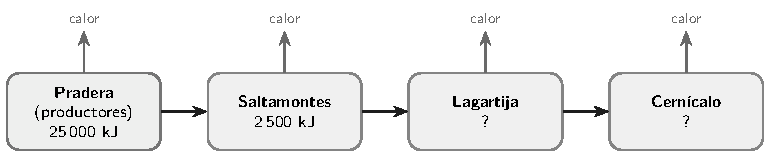
\includegraphics[max width=0.92\linewidth,max height=8.5cm]{bio/amb_energia_q}
\end{center}
\alts{2 500 kJ}{250 kJ}{25 kJ}{2,5 kJ}
\solucion{\textbf{Paso 1. ¿Qué nos piden?} La energía del cuarto nivel (cernícalo), sabiendo que pasa cerca del 10 \% de un nivel al siguiente.

\textbf{Paso 2. Comprueba la regla con los datos.} De la pradera (25 000 kJ) a los saltamontes (2 500 kJ) pasa el 10 \%. Se cumple.

\textbf{Paso 3. Sigue la cadena.} Lagartija: 10 \% de 2 500 = 250 kJ. Cernícalo: 10 \% de 250 = 25 kJ.

\textbf{Respuesta:} 25 kJ.

\textbf{¿Por qué no las otras?} 2 500 kJ es la energía de los saltamontes. 250 kJ es la de la lagartija: falta un paso. 2,5 kJ supone un paso de más, como si hubiera un quinto nivel.

\textbf{\color{cienciaD}Para recordar.} Cada paso hacia arriba en la cadena multiplica la energía por cerca de 0,1.}{C}
\end{elejemplo}
\motivacion{La energía fluye y la materia circula. Tu aprendizaje también fluye: ya casi terminas Biología.}

\chapter{Habilidades científicas}
%% =====================================================================
%% bio_hab_investigacion
\section[Preguntas, hipótesis y variables]{Preguntas, hipótesis y variables}
\modcomun\ \ {\color{gris}\itshape Cómo se arma una investigación en biología: pregunta investigable, hipótesis y predicción, variables independiente, dependiente y controladas, grupo control, componentes de una investigación (teoría, ley, modelo, objetivo, resultado, inferencia, conclusión) y un procedimiento que cambie solo una variable.\par}
\subsection{La investigación científica paso a paso}
Entre un cuarto y un tercio de las preguntas de la PAES de Ciencias no miden cuánta biología sabes, sino si sabes \textbf{pensar como investigador}: reconocer la pregunta, la hipótesis, las variables y la conclusión de un estudio. Todas siguen el mismo esquema:

 
\begin{center}
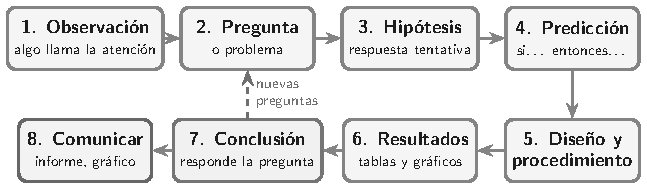
\includegraphics[max width=0.92\linewidth,max height=8.5cm]{bio/hab_ciclo}
\end{center}
  

\textbf{Un ejemplo completo.}

 

\textbf{1. Observación.} Una estudiante nota que las semillas de rabanito brotan antes en primavera que en invierno.

 

\textbf{2. Pregunta.} ¿Cómo influye la temperatura en la germinación de las semillas de rabanito?

 

\textbf{3. Hipótesis.} La temperatura influye en el porcentaje de semillas que germinan.

 

\textbf{4. Predicción.} Si la hipótesis es correcta, a 20 °C germinará un porcentaje distinto de semillas que a 10 °C.

 

\textbf{5. Procedimiento.} Pone 10 semillas en placas con papel húmedo a 10, 20, 30 y 40 °C, y después de 4 días cuenta las semillas germinadas.

 

\textbf{6. Resultados.} 20 \%, 70 \%, 90 \% y 30 \%.

 

\textbf{7. Conclusión.} En el rango estudiado, la temperatura influyó en la germinación: el mayor porcentaje se obtuvo a 30 °C.

  
\begin{clave}[{Pregunta investigable}] Es una pregunta que se puede responder \textbf{midiendo} u observando algo. Casi siempre relaciona dos variables: «¿cómo influye A en B?».\end{clave}
 
\begin{clave}[{¿Investigable o no?}] · «¿Influye la cantidad de luz en el crecimiento de una planta de poroto?»: sí, se mide la altura.\par · «¿Es el colibrí el ave más hermosa de Chile?»: no, es una opinión.\par · «¿Qué especies existirán dentro de un millón de años?»: no, no se puede medir hoy.\end{clave}
 
\begin{clave}[{Recuerda}] La pregunta de investigación calza con los datos. Si en la tabla solo cambia la especie de planta y se mide la altura, la pregunta es «¿cómo varía la altura entre estas especies?».\end{clave}
\subsection{Hipótesis y predicción}
La \textbf{hipótesis} es una explicación o respuesta tentativa a la pregunta. Tiene tres rasgos:

 
\begin{itemize}
  \item Se escribe \textbf{antes} del experimento.
  \item Relaciona la variable que se cambia con la que se mide: «la temperatura influye en la actividad de la levadura», «a mayor intensidad de luz, mayor tasa de fotosíntesis».
  \item Se puede poner a prueba, y podría resultar falsa.
\end{itemize}
 

La \textbf{predicción} es más concreta: dice qué resultado se espera en \textbf{este} experimento si la hipótesis es cierta. Suele tener la forma «si\dots{}, entonces\dots{}».

 
\begin{center}\small
\begin{tabularx}{\linewidth}{@{}>{\raggedright\arraybackslash\hsize=1.00\hsize}X>{\raggedright\arraybackslash\hsize=1.00\hsize}X@{}}
\toprule
\textbf{Hipótesis} & \textbf{Predicción} \\
\midrule
La intensidad de luz influye en la tasa de fotosíntesis de \emph{Elodea}. & Con la lámpara a 10 cm, la rama liberará más burbujas por minuto que con la lámpara a 40 cm. \\
La temperatura influye en la producción de CO\textsubscript{2} de la levadura. & El globo del matraz a 35 °C se inflará más que el del matraz a 10 °C. \\
\bottomrule
\end{tabularx}
\end{center}
  
\begin{ejemplo}[{Ejemplo resuelto: ¿qué hipótesis se puso a prueba?}] Unos estudiantes riegan cuatro grupos de plantas de lechuga con agua que tiene 0, 1, 2 y 4 g/L de sal. Todas son de la misma edad, están en el mismo invernadero y reciben el mismo volumen de agua. Después de 3 semanas miden la masa de cada planta.\par \textbf{Paso 1.} ¿Qué cambia de un grupo a otro? Solo la concentración de sal del agua de riego.\par \textbf{Paso 2.} ¿Qué se mide? La masa de las plantas.\par \textbf{Paso 3.} La hipótesis une las dos: «la concentración de sal del agua de riego influye en el crecimiento de la lechuga».\par Una hipótesis sobre la luz, la edad de las plantas o el volumen de riego no se puede probar aquí: esas variables se mantuvieron iguales.\end{ejemplo}
 
\begin{clave}[{Recuerda}] La hipótesis va antes de experimentar; la conclusión, después, apoyada en los datos. Un experimento no «demuestra» una hipótesis para siempre: la apoya o la contradice.\end{clave}
\subsection{Variables: independiente, dependiente y controladas}
\begin{center}
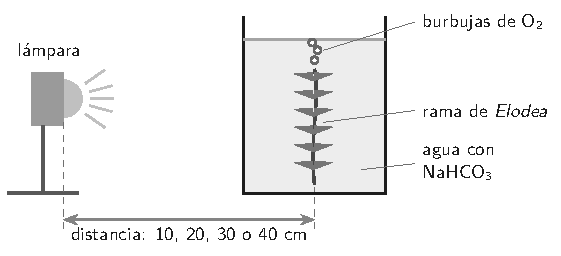
\includegraphics[max width=0.92\linewidth,max height=8.5cm]{bio/hab_elodea}
\end{center}
  

En el montaje, un grupo pone una rama de \emph{Elodea} (planta acuática) en agua con bicarbonato de sodio, que aporta CO\textsubscript{2}. Ubica la lámpara a distintas distancias y cuenta las burbujas de O\textsubscript{2} que libera la rama en un minuto.

 
\begin{center}\small
\begin{tabularx}{\linewidth}{@{}>{\raggedright\arraybackslash\hsize=0.50\hsize}X>{\raggedright\arraybackslash\hsize=1.25\hsize}X>{\raggedright\arraybackslash\hsize=1.25\hsize}X@{}}
\toprule
\textbf{Variable} & \textbf{Cómo reconocerla} & \textbf{En el montaje} \\
\midrule
\textbf{Independiente} & La que el investigador \textbf{cambia a propósito} (la causa). & Distancia de la lámpara, es decir, la intensidad de luz \\
\textbf{Dependiente} & La que se \textbf{mide} como respuesta (el efecto). & Burbujas de O\textsubscript{2} por minuto \\
\textbf{Controladas} & Las que se dejan \textbf{iguales} para que no influyan. & Rama de la misma planta, temperatura del agua, cantidad de bicarbonato, tiempo de conteo \\
\bottomrule
\end{tabularx}
\end{center}
  
\gatotip[\gatogris]{\textbf{Truco de la frase.} Arma la frase «el efecto de \textbf{[independiente]} sobre \textbf{[dependiente]}». Aquí: «el efecto de la intensidad de luz sobre la liberación de O\textsubscript{2}». Si la frase no tiene sentido, cambiaste el orden.}
 
\begin{ejemplo}[{Ejemplo resuelto}] Se cultivan bacterias en placas con 0, 5, 10 y 20 mg/L de un antibiótico, todas a 37 °C, y después de 24 h se cuentan las colonias.\par · Cambia a propósito: la concentración de antibiótico \ensuremath{\rightarrow} \textbf{independiente}.\par · Se mide al final: el número de colonias \ensuremath{\rightarrow} \textbf{dependiente}.\par · Siempre igual: la temperatura (37 °C) y el tiempo (24 h) \ensuremath{\rightarrow} \textbf{controladas}.\end{ejemplo}
 
\begin{clave}[{Recuerda}] Para encontrar la variable independiente, pregúntate qué decidió el investigador \textbf{antes} de medir. La dependiente es lo que registra al final, muchas veces con un instrumento.\end{clave}
\subsection{Grupo control, comparaciones justas e instrumentos}
El \textbf{grupo control} es el grupo de comparación: igual a los demás, pero \textbf{sin} el factor que se estudia. Si quieres probar que un fertilizante aumenta el crecimiento del tomate, necesitas plantas con fertilizante y otras plantas iguales, con el mismo riego, luz y suelo, pero sin fertilizante. Sin ese grupo no sabes si el fertilizante hizo algo.

 

En los estudios con personas, el grupo control suele recibir un \textbf{placebo}: una pastilla igual, pero sin el fármaco, para que la sola idea de estar tratado no influya en el resultado.

 

\textbf{Compara solo grupos que se diferencian en una cosa.}

 
\begin{center}\small
\begin{tabular}{@{}lll@{}}
\toprule
\textbf{Grupo} & \textbf{Temperatura} & \textbf{Luz} \\
\midrule
1 & 20 °C & 12 h/día \\
2 & 30 °C & 12 h/día \\
3 & 30 °C & 16 h/día \\
\bottomrule
\end{tabular}
\end{center}
 

· 1 y 2: solo cambia la temperatura \ensuremath{\rightarrow} sirven para estudiar la temperatura.\par · 2 y 3: solo cambian las horas de luz \ensuremath{\rightarrow} sirven para estudiar la luz.\par · 1 y 3: cambian dos cosas \ensuremath{\rightarrow} no permiten saber cuál causó la diferencia.

  
\begin{clave}[{Instrumentos según la variable}] \begin{center}\small
\begin{tabularx}{\linewidth}{@{}>{\raggedright\arraybackslash\hsize=1.00\hsize}X>{\raggedright\arraybackslash\hsize=1.00\hsize}X@{}}
\toprule
\textbf{Para medir\dots{}} & \textbf{se usa\dots{}} \\
\midrule
masa (de una planta, de una semilla) & balanza \\
longitud (altura de un tallo, largo de una raíz) & regla o huincha \\
volumen de un líquido & probeta o pipeta \\
volumen de un gas (CO\textsubscript{2}, O\textsubscript{2}) & jeringa o probeta invertida \\
temperatura & termómetro \\
tiempo & cronómetro \\
acidez & pHmetro o papel indicador \\
frecuencia cardíaca & pulsómetro, o contar el pulso con un cronómetro \\
células, estructuras pequeñas & microscopio \\
\bottomrule
\end{tabularx}
\end{center}\end{clave}
 
\begin{clave}[{Recuerda}] Antes de elegir un instrumento, identifica qué variable piden. Si se calienta un cultivo y se cuentan sus colonias, el termómetro mide la variable independiente y el conteo de colonias es la dependiente.\end{clave}
\subsection{Teoría, ley, modelo y los demás componentes}
La PAES pregunta mucho «¿a qué componente de la investigación corresponde la frase entre comillas?». Apréndete esta tabla:

 
\begin{center}\small
\begin{tabularx}{\linewidth}{@{}>{\raggedright\arraybackslash\hsize=0.62\hsize}X>{\raggedright\arraybackslash\hsize=1.19\hsize}X>{\raggedright\arraybackslash\hsize=1.19\hsize}X@{}}
\toprule
\textbf{Componente} & \textbf{Qué es} & \textbf{Ejemplo en biología} \\
\midrule
\textbf{Teoría} & Explica \textbf{por qué} pasa algo; está respaldada por mucha evidencia. & Teoría celular; teoría de la evolución por selección natural. \\
\textbf{Ley} & Describe una regularidad: \textbf{qué} pasa, sin explicar por qué. & Leyes de Mendel (segregación, distribución independiente). \\
\textbf{Modelo} & Representación simplificada para explicar o predecir. & Modelo del mosaico fluido de la membrana; modelo de doble hélice del ADN; modelo llave-cerradura de las enzimas. \\
\textbf{Marco conceptual} & Lo que ya se sabe del tema: teorías, leyes, modelos y antecedentes. & «La insulina disminuye la glucosa en la sangre». \\
\textbf{Problema / pregunta} & Lo que se quiere averiguar. & «¿Cómo afecta la sal del suelo al crecimiento de la lechuga?». \\
\textbf{Objetivo} & Lo que se quiere lograr; empieza con un verbo en infinitivo. & «Determinar el efecto de la temperatura en la germinación del trigo». \\
\textbf{Procedimiento} & Los pasos que se siguen. & «Se sembraron 10 semillas por placa y se incubaron a 20 °C\dots{}». \\
\textbf{Resultado / evidencia} & Los datos obtenidos. & «Germinaron 9 de 10 semillas a 30 °C». \\
\textbf{Inferencia} & Interpretación que va más allá de lo observado. & «Las guarderías de polluelos podrían aumentar su sobrevivencia». \\
\textbf{Conclusión} & Respuesta a la pregunta, apoyada en los resultados. & «En el rango estudiado, la germinación fue máxima a 30 °C». \\
\bottomrule
\end{tabularx}
\end{center}
  
\begin{clave}[{Pistas en el texto}] · «si\dots{}, entonces\dots{} ocurrirá»: predicción.\par · «determinar», «evaluar», «comparar», en infinitivo: objetivo.\par · «se agregó, se sembró, se midió»: procedimiento.\par · «se obtuvo», «los valores fueron»: resultado.\par · «esto sugiere», «podría indicar»: inferencia.\par · «por lo tanto», en respuesta a la pregunta: conclusión.\end{clave}
  
\begin{clave}[{Recuerda}] Una ley dice qué pasa y una teoría explica por qué pasa. Son componentes distintos: la teoría celular explica la organización de los seres vivos con mucha evidencia, y las leyes de Mendel describen cómo se reparten los caracteres en la descendencia.\end{clave}
\subsection{Diseñar un procedimiento que cambie solo una variable}
\begin{center}
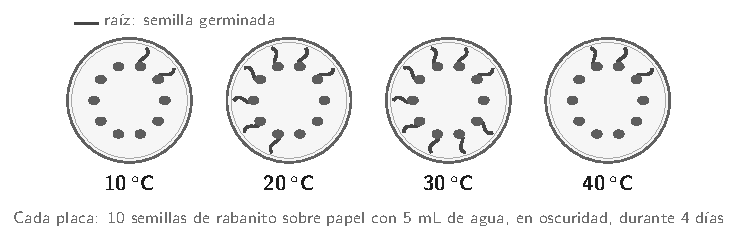
\includegraphics[max width=0.92\linewidth,max height=8.5cm]{bio/hab_germinacion}
\end{center}
  

Un buen procedimiento sigue cinco pasos:

 

\textbf{Paso 1.} Lee el objetivo y nombra la variable independiente (la que vas a cambiar) y la dependiente (la que vas a medir).

 

\textbf{Paso 2.} Elige varios valores de la independiente, bien separados: 10, 20, 30 y 40 °C.

 

\textbf{Paso 3.} Deja \textbf{todo lo demás igual}: misma especie, mismo número de semillas, misma agua, misma luz, mismo tiempo.

 

\textbf{Paso 4.} Decide cómo y con qué medirás la dependiente: contar semillas germinadas al cuarto día.

 

\textbf{Paso 5.} Repite cada condición (varias placas por temperatura) para que el resultado no dependa de una sola placa.

  
\begin{ejemplo}[{Ejemplo resuelto}] En las placas de la figura se ve: 10 °C, 2 de 10 germinadas (20 \%); 20 °C, 7 de 10 (70 \%); 30 °C, 9 de 10 (90 \%); 40 °C, 3 de 10 (30 \%).\par Como en todas las placas hay la misma especie, el mismo número de semillas, la misma agua y la misma oscuridad, la diferencia se puede atribuir a la temperatura.\end{ejemplo}
 
\begin{clave}[{Recuerda}] Si dos grupos difieren en dos variables a la vez (por ejemplo, temperatura y cantidad de agua), no se puede saber cuál de las dos causó la diferencia. Por eso cada ensayo cambia solo la variable independiente.\end{clave}
\subsection{Lo clave del tema}
\begin{center}\small
\begin{tabularx}{\linewidth}{@{}>{\raggedright\arraybackslash\hsize=0.77\hsize}X>{\raggedright\arraybackslash\hsize=1.23\hsize}X@{}}
\toprule
\textbf{Concepto} & \textbf{Lo que tienes que reconocer} \\
\midrule
Pregunta de investigación & Se responde midiendo; calza con lo que se varió y lo que se midió. \\
Hipótesis & Respuesta tentativa que relaciona la variable independiente con la dependiente. \\
Predicción & Resultado concreto esperado: «si\dots{}, entonces\dots{}». \\
Variable independiente & La que se cambia a propósito. \\
Variable dependiente & La que se mide. \\
Variables controladas & Las que se mantienen iguales. \\
Grupo control & Grupo igual a los demás, pero sin el factor estudiado. \\
Teoría / ley / modelo & Por qué pasa / qué pasa / representación simplificada. \\
\bottomrule
\end{tabularx}
\end{center}
 
\begin{clave}[{Recuerda}] · Variable independiente: la que se decide antes; dependiente: la que se mide.\par · La hipótesis habla de la variable que cambia en el experimento.\par · Para estudiar una variable, compara grupos que solo difieren en esa variable.\par · «Germinaron 9 de 10 semillas» es un resultado; la conclusión lo interpreta y responde la pregunta.\par · El objetivo se escribe con un verbo en infinitivo: determinar, evaluar, comparar.\end{clave}
 
\begin{clave}[{Método PAES}] 1. Subraya qué se cambió, qué se midió y qué se dejó igual. 2. Con eso, nombra las tres variables. 3. Si preguntan por la hipótesis o la pregunta, elige la que relaciona exactamente esas dos variables. 4. Si preguntan por un componente, busca las pistas («si\dots{} entonces», «determinar», «se obtuvo», «se sembró»). 5. Descarta las alternativas que hablan de variables que no cambiaron o que no se midieron.\end{clave}
\begin{elejemplo}{Estilo PAES}
Un grupo de estudiantes quiere averiguar qué factores influyen en el crecimiento de plantas de poroto. Para ello prepara cuatro ensayos con plantas de la misma edad y en el mismo tipo de suelo, como se muestra en la figura. Después de tres semanas medirá la altura de las plantas.

¿Cuál de las siguientes comparaciones permite estudiar el efecto de un solo factor?
\begin{center}
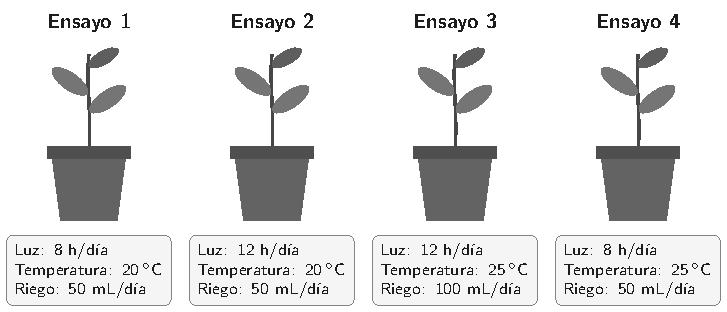
\includegraphics[max width=0.92\linewidth,max height=8.5cm]{bio/hab_macetas}
\end{center}
\altslargas{Comparar los ensayos 1 y 3 permite analizar el efecto del riego.}{Comparar los ensayos 2 y 4 permite analizar el efecto de la temperatura.}{Comparar los ensayos 1 y 4 permite analizar el efecto de la temperatura.}{Comparar los ensayos 3 y 4 permite analizar el efecto de las horas de luz.}
\solucion{\textbf{Paso 1. ¿Qué nos piden?} Un par de ensayos que sirva para estudiar el efecto de \textbf{un} factor. Dos ensayos sirven para estudiar una variable solo si se diferencian \textbf{únicamente} en esa variable. Así, si la altura cambia, sabemos qué lo causó.

\textbf{Paso 2. Ensayos 1 y 3.} Luz: 8 y 12 h (cambia). Temperatura: 20 y 25 °C (cambia). Riego: 50 y 100 mL (cambia). Cambian los tres factores: este par no sirve.

\textbf{Paso 3. Ensayos 2 y 4.} Luz: 12 y 8 h (cambia). Temperatura: 20 y 25 °C (cambia). Riego: 50 y 50 mL (igual). Cambian dos factores: no sirve.

\textbf{Paso 4. Ensayos 1 y 4.} Luz: 8 y 8 h (igual). Temperatura: 20 y 25 °C (cambia). Riego: 50 y 50 mL (igual). Solo cambia la temperatura: este par sirve para estudiar la \textbf{temperatura}.

\textbf{Paso 5. Ensayos 3 y 4.} Luz: 12 y 8 h (cambia). Temperatura: 25 y 25 °C (igual). Riego: 100 y 50 mL (cambia). Cambian dos factores: no sirve.

\textbf{Respuesta:} comparar los ensayos 1 y 4 permite analizar el efecto de la temperatura.

\textbf{Comprobación:} en los ensayos 1 y 4 la temperatura es la variable independiente, y la luz (8 h) y el riego (50 mL/día) son variables controladas. También los ensayos 1 y 2 forman un buen par, pero para estudiar la luz, y esa comparación no está entre las alternativas.

\textbf{¿Por qué no las otras?} «1 y 3 para el riego» elige un par en que cambian los tres factores. «2 y 4 para la temperatura» y «3 y 4 para la luz» eligen pares en que cambian dos factores a la vez; cualquier diferencia en la altura podría deberse a cualquiera de los dos.

\textbf{\color{cienciaD}Para recordar.} Para estudiar una variable, compara solo ensayos que se diferencian únicamente en esa variable.}{C}
\end{elejemplo}
\motivacion{Hipótesis, variables y grupo control: ya diseñas experimentos con orden. La biología también es método.}

%% =====================================================================
%% bio_hab_evidencia
\section[Procesar y analizar evidencia]{Procesar y analizar evidencia}
\modcomun\ \ {\color{gris}\itshape Leer tablas y gráficos de líneas, barras, circulares y de dispersión con datos biológicos, reconocer relaciones directas, inversas y proporcionales, tendencias, máximos y óptimos (como la actividad enzimática según el pH o la temperatura), hacer predicciones e inferencias y calcular promedios y variaciones.\par}
\subsection{Leer una tabla de datos}
Antes de mirar las alternativas, lee la tabla en cuatro pasos:

 

\textbf{Paso 1. Encabezados y unidades.} ¿Qué mide cada columna? ¿En qué unidad?

 

\textbf{Paso 2. ¿Qué cambia y qué se mide?} Identifica la variable independiente y la dependiente.

 

\textbf{Paso 3. Recorre en orden.} Sigue la columna que crece y mira qué hace la otra: ¿sube, baja o queda igual?

 

\textbf{Paso 4. Revisa todas las filas.} Una tendencia vale solo si se cumple en todas.

 
\begin{center}\small
\begin{tabularx}{\linewidth}{@{}>{\raggedright\arraybackslash\hsize=0.85\hsize}X>{\raggedright\arraybackslash\hsize=0.78\hsize}X>{\raggedright\arraybackslash\hsize=1.36\hsize}X@{}}
\toprule
\textbf{Temperatura del agua (°C)} & \textbf{Oxígeno disuelto (mg/L)} & \textbf{Movimientos del opérculo de un pez (por min)} \\
\midrule
5 & 12,8 & 40 \\
10 & 11,3 & 55 \\
15 & 10,1 & 70 \\
20 & 9,1 & 90 \\
\bottomrule
\end{tabularx}
\end{center}
  
\begin{ejemplo}[{Ejemplo resuelto}] En la tabla, la temperatura crece de arriba hacia abajo: 5 \ensuremath{\rightarrow} 10 \ensuremath{\rightarrow} 15 \ensuremath{\rightarrow} 20 °C. Mientras tanto, el oxígeno disuelto baja (12,8 \ensuremath{\rightarrow} 9,1 mg/L) y los movimientos del opérculo, con los que el pez hace pasar agua por sus branquias, suben (40 \ensuremath{\rightarrow} 90 por minuto).\par Relaciones correctas:\par · «El oxígeno disuelto \textbf{disminuye} al aumentar la temperatura» (relación inversa).\par · «Los movimientos del opérculo \textbf{aumentan} al disminuir el oxígeno disuelto» (también inversa, leída al revés).\par Una inferencia razonable: con menos oxígeno en el agua, el pez mueve más agua por sus branquias.\end{ejemplo}
 
\begin{clave}[{Recuerda}] Cuando una alternativa recorre la tabla al revés («al disminuir\dots{}»), recórrela tú también al revés antes de responder. En una relación inversa, si una variable baja, la otra sube.\end{clave}
\subsection{Leer un gráfico: máximos y óptimos}
\begin{center}
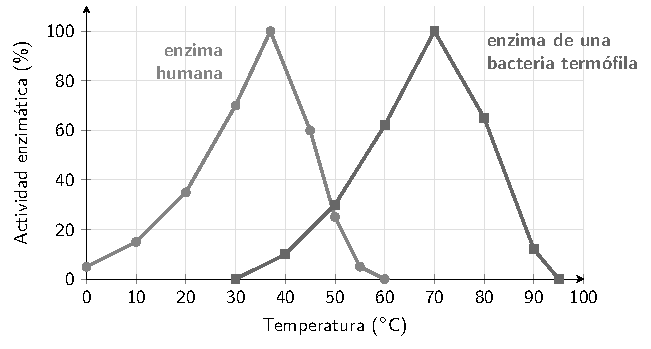
\includegraphics[max width=0.92\linewidth,max height=8.5cm]{bio/hab_enzima_temp}
\end{center}
 

\textbf{Paso 1. Ejes.} Eje horizontal: temperatura (°C), la variable independiente. Eje vertical: actividad enzimática (\%), la variable dependiente.

 

\textbf{Paso 2. Escala.} Cada línea vertical vale 10 °C; cada horizontal, 20 \%.

 

\textbf{Paso 3. Lee puntos.} La enzima humana tiene 35 \% de actividad a 20 °C, 100 \% a 37 °C y 25 \% a 50 °C.

 

\textbf{Paso 4. Busca el máximo.} La temperatura en que la actividad es máxima es la \textbf{temperatura óptima}: 37 °C para la enzima humana y 70 °C para la de la bacteria termófila, que vive en aguas termales.

  
\begin{clave}[{La forma de la curva cuenta la historia}] Bajo el óptimo, la actividad sube con la temperatura, porque las moléculas se mueven más rápido y se encuentran más. Sobre el óptimo, la actividad cae bruscamente: la enzima se \textbf{desnaturaliza}, es decir, pierde su forma y deja de funcionar.\end{clave}
 
\begin{ejemplo}[{Ejemplo resuelto}] ¿A qué temperaturas la enzima humana tiene más de la mitad de su actividad máxima?\par \textbf{Paso 1.} La mitad de 100 \% es 50 \%.\par \textbf{Paso 2.} La curva supera el 50 \% entre unos 25 °C y unos 47 °C.\par \textbf{Paso 3.} En ese rango la actividad es mayor que 50 \%.\end{ejemplo}
 
\begin{clave}[{Recuerda}] Para comparar dos curvas, léelas en el mismo valor del eje horizontal. A 60 °C la enzima bacteriana tiene 62 \% de actividad y la humana, 0 \%.\end{clave}
\subsection{Tipos de gráfico y cuándo usarlos}
\begin{center}
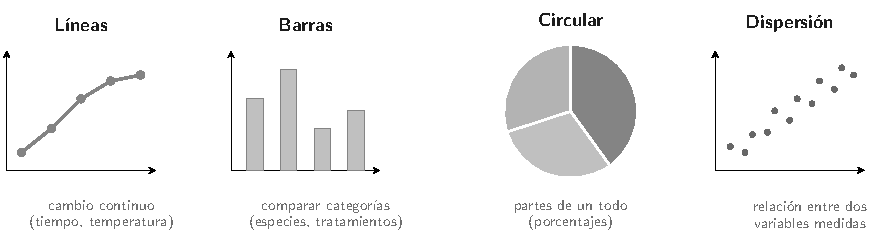
\includegraphics[max width=0.92\linewidth,max height=8.5cm]{bio/hab_graficos}
\end{center}
  
\begin{center}\small
\begin{tabularx}{\linewidth}{@{}>{\raggedright\arraybackslash\hsize=0.42\hsize}X>{\raggedright\arraybackslash\hsize=1.29\hsize}X>{\raggedright\arraybackslash\hsize=1.29\hsize}X@{}}
\toprule
\textbf{Gráfico} & \textbf{Sirve para\dots{}} & \textbf{Ejemplo en biología} \\
\midrule
\textbf{Líneas} & Mostrar cómo cambia una variable a lo largo de otra continua (tiempo, temperatura, pH). & Frecuencia cardíaca durante el ejercicio; crecimiento de una población bacteriana. \\
\textbf{Barras} & Comparar valores entre categorías separadas. & Porcentaje de germinación de cuatro especies. \\
\textbf{Circular} & Mostrar cómo se reparte un total (100 \%) entre sus partes. & Porcentaje de cada tipo de glóbulo blanco en la sangre. \\
\textbf{Dispersión} & Ver si dos variables medidas en muchos individuos se relacionan. & Masa corporal y frecuencia cardíaca de distintos mamíferos. \\
\bottomrule
\end{tabularx}
\end{center}
  
\begin{clave}[{Dónde va cada variable}] En los gráficos de líneas y de dispersión, la variable independiente va en el eje horizontal y la dependiente en el vertical.\end{clave}
 
\begin{ejemplo}[{Ejemplo resuelto}] Un estudiante cuenta los individuos de cinco especies de aves en un humedal. ¿Qué gráfico usa para compararlas?\par Las especies son categorías separadas, sin un orden numérico entre ellas: un \textbf{gráfico de barras}, con una barra por especie.\end{ejemplo}
\subsection{Relaciones entre variables}
\begin{center}
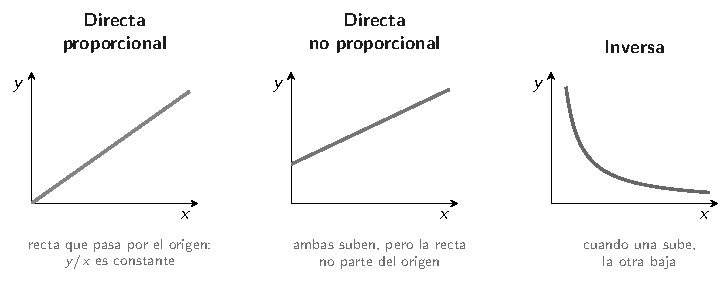
\includegraphics[max width=0.92\linewidth,max height=8.5cm]{bio/hab_relaciones}
\end{center}
  
\begin{center}\small
\begin{tabularx}{\linewidth}{@{}>{\raggedright\arraybackslash\hsize=0.71\hsize}X>{\raggedright\arraybackslash\hsize=1.14\hsize}X>{\raggedright\arraybackslash\hsize=1.14\hsize}X@{}}
\toprule
\textbf{Relación} & \textbf{Qué pasa} & \textbf{Cómo comprobarla} \\
\midrule
Directa & Si una aumenta, la otra también. & Ambas columnas suben juntas. \\
Directamente proporcional & Si una se duplica, la otra se duplica. & El cociente $y/x$ es constante; el gráfico es una recta que pasa por el origen. \\
Inversa & Si una aumenta, la otra disminuye. & Una columna sube y la otra baja. \\
Inversamente proporcional & Si una se duplica, la otra se reduce a la mitad. & El producto $x\cdot y$ es constante. \\
\bottomrule
\end{tabularx}
\end{center}
  
\begin{ejemplo}[{Ejemplo resuelto}] Distintas cantidades de una enzima digieren un trozo igual de gelatina, a la misma temperatura:
\begin{center}\small
\begin{tabular}{@{}lll@{}}
\toprule
\textbf{Enzima (u.a.)} & \textbf{Tiempo (min)} & \textbf{Enzima × tiempo} \\
\midrule
1 & 60 & 60 \\
2 & 30 & 60 \\
3 & 20 & 60 \\
\bottomrule
\end{tabular}
\end{center}
 El producto es siempre 60: el tiempo de digestión es \textbf{inversamente proporcional} a la cantidad de enzima.\end{ejemplo}
 
\begin{clave}[{Recuerda}] Una relación es proporcional solo si el cociente (directa) o el producto (inversa) es constante. La altura de una planta sube con los días, pero si la semilla ya medía 2 cm el primer día, la recta no pasa por el origen: es directa, no proporcional.\end{clave}
\subsection{Tendencias: interpolar y predecir}
Una \textbf{tendencia} es el patrón que siguen los datos. Con ella se puede estimar un valor que no se midió.

 
\begin{itemize}
  \item \textbf{Interpolar}: estimar un valor \textbf{dentro} del rango medido. Es bastante seguro.
  \item \textbf{Extrapolar}: estimar \textbf{fuera} del rango medido. Es arriesgado y solo vale para valores cercanos.
\end{itemize}
 
\begin{center}\small
\begin{tabular}{@{}ll@{}}
\toprule
\textbf{pH del suelo} & \textbf{Crecimiento de una planta de maíz (cm/semana)} \\
\midrule
4 & 2 \\
5 & 5 \\
6 & 8 \\
7 & 7 \\
8 & 3 \\
\bottomrule
\end{tabular}
\end{center}
 

El crecimiento sube hasta pH 6 y luego baja: hay un \textbf{óptimo} cerca de pH 6. A pH 6,5 se espera un valor entre 7 y 8 cm por semana (interpolación).

  
\begin{ejemplo}[{Ejemplo resuelto: predecir con la tendencia}] Una lagartija, cuya temperatura corporal depende del ambiente, consume 0,10 mL de O\textsubscript{2} por gramo y por hora a 10 °C; 0,20 a 20 °C, y 0,40 a 30 °C.\par \textbf{Paso 1.} Cada 10 °C, el consumo se duplica.\par \textbf{Paso 2.} A 25 °C, el consumo debe estar entre 0,20 y 0,40: unos 0,3 mL de O\textsubscript{2} por gramo y por hora.\end{ejemplo}
 
\begin{clave}[{Recuerda}] Una predicción se apoya en la tendencia medida y se limita al rango estudiado o a valores cercanos. Si el maíz se midió entre pH 4 y 8, los datos no dicen qué pasa a pH 2.\end{clave}
\subsection{Cálculos simples: promedio, variación y porcentaje}
Muchas preguntas de evidencia piden un cálculo corto antes de comparar. Sin calculadora, ordena los pasos:

 
\begin{center}\small
\begin{tabularx}{\linewidth}{@{}>{\raggedright\arraybackslash\hsize=0.67\hsize}X>{\raggedright\arraybackslash\hsize=1.33\hsize}X@{}}
\toprule
\textbf{Cálculo} & \textbf{Cómo se hace} \\
\midrule
Promedio & Suma de los valores dividida por cuántos son. \\
Variación & Valor final \ensuremath{-} valor inicial. \\
Variación porcentual & $\dfrac{\text{final} - \text{inicial}}{\text{inicial}}\cdot 100$ \\
Tasa o rapidez & Variación dividida por el tiempo. \\
Eficiencia & Lo obtenido dividido por lo usado. \\
\bottomrule
\end{tabularx}
\end{center}
  
\begin{ejemplo}[{Ejemplo resuelto: promedio de repeticiones}] Tres plantas regadas con un fertilizante crecieron 12, 14 y 13 cm. Promedio: $\dfrac{12 + 14 + 13}{3} = \dfrac{39}{3} = 13$ cm. Un valor aislado alto, como 19 cm en una sola planta, no basta para decir que un tratamiento es mejor: se comparan los promedios.\end{ejemplo}
 
\begin{ejemplo}[{Ejemplo resuelto: variación porcentual}] Una población de 200 coipos pasa a 250 en un año. Variación: $250 - 200 = 50$. Variación porcentual: $\dfrac{50}{200}\cdot 100 = 25\%$. Se divide por el valor \textbf{inicial}.\end{ejemplo}
 
\begin{clave}[{Recuerda}] «Más eficiente», «mayor rendimiento» y «mayor aumento porcentual» piden un cociente, no el número más grande de la tabla.\end{clave}
\subsection{Lo clave del tema}
\begin{center}\small
\begin{tabularx}{\linewidth}{@{}>{\raggedright\arraybackslash\hsize=1.00\hsize}X>{\raggedright\arraybackslash\hsize=1.00\hsize}X@{}}
\toprule
\textbf{Si te piden\dots{}} & \textbf{Haz esto} \\
\midrule
Una relación o tendencia & Recorre la variable que crece y mira qué hace la otra; revisa todas las filas. \\
Saber si es proporcional & Directa: cociente constante, recta por el origen. Inversa: producto constante. \\
Leer un gráfico & Ejes, unidades y escala antes de leer un punto. \\
Un óptimo & Busca el valor del eje horizontal donde la curva es más alta. \\
Una predicción & Sigue la tendencia, sin extrapolar lejos del rango medido. \\
Una conclusión o inferencia & Que salga de los datos, hable solo de lo medido y no agregue nada. \\
Un promedio, una variación o una eficiencia & Calcula para cada grupo y después compara. \\
\bottomrule
\end{tabularx}
\end{center}
 
\begin{clave}[{Recuerda}] · En una relación inversa, cuando una variable disminuye, la otra aumenta.\par · Cada enzima tiene un óptimo de temperatura y de pH; lejos del óptimo, su actividad baja.\par · Que dos variables cambien juntas no prueba que una cause la otra.\par · La conclusión se limita a lo estudiado: «en el rango estudiado, la germinación fue máxima a 30 °C».\par · La variación porcentual se calcula sobre el valor inicial.\end{clave}
 
\begin{clave}[{Método PAES}] 1. Lee encabezados, ejes y unidades. 2. Identifica qué cambió y qué se midió. 3. Describe en tu cabeza la tendencia antes de leer las alternativas. 4. Si hay números, calcula el promedio, la diferencia, el cociente o el producto que corresponda. 5. Descarta lo que no sale de los datos, lo que generaliza y lo que habla de variables que no se midieron.\end{clave}
\begin{elejemplo}{PAES Regular 2026, adaptada}
En un laboratorio se mide la actividad de dos enzimas digestivas humanas a distintos valores de pH, manteniendo la temperatura en 37 °C. La pepsina actúa en el estómago y la amilasa salival, en la boca. Los resultados se muestran en el gráfico:

¿Cuál de las siguientes afirmaciones describe correctamente los resultados?
\begin{center}
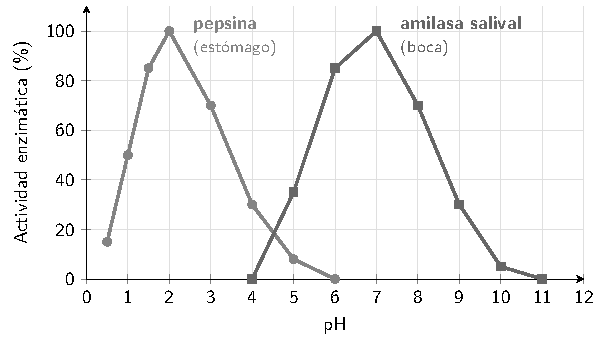
\includegraphics[max width=0.92\linewidth,max height=8.5cm]{bio/hab_enzima_ph}
\end{center}
\altslargas{Ambas enzimas alcanzan su máxima actividad al mismo pH.}{A pH 7, la pepsina alcanza su máxima actividad.}{Cada enzima tiene un pH óptimo, y su actividad disminuye al alejarse de él hacia valores más ácidos o más básicos.}{La actividad de la amilasa salival aumenta siempre al aumentar el pH.}
\solucion{\textbf{Paso 1. ¿Qué nos piden?} La afirmación que describe bien el gráfico. Primero lo leemos y después revisamos cada alternativa.

\textbf{Paso 2. Lee los ejes.} Eje horizontal: pH, de 0 a 12. Eje vertical: actividad enzimática en \%. Cada línea horizontal vale 20 \%.

\textbf{Paso 3. Lee la pepsina.} Sube desde pH 0,5 hasta su máximo (100 \%) a pH 2 y luego baja hasta 0 \% a pH 6.

\textbf{Paso 4. Lee la amilasa.} Es 0 \% a pH 4, sube hasta 100 \% a pH 7 y baja hasta 0 \% a pH 11.

\textbf{Paso 5. Describe la tendencia.} Las dos curvas tienen un máximo, el \textbf{pH óptimo}: 2 para la pepsina y 7 para la amilasa. A ambos lados del óptimo, la actividad disminuye.

\textbf{Respuesta:} cada enzima tiene un pH óptimo, y su actividad disminuye al alejarse de él hacia valores más ácidos o más básicos.

\textbf{Comprobación:} los óptimos calzan con el lugar donde actúa cada enzima. El estómago es muy ácido (pH cercano a 2) y la boca es casi neutra (pH cercano a 7).

\textbf{¿Por qué no las otras?} «Al mismo pH» es falsa: los máximos están en pH 2 y en pH 7. «A pH 7 la pepsina alcanza su máximo» es falsa: a pH 7 la pepsina tiene 0 \% de actividad. «La amilasa aumenta siempre» solo se cumple hasta pH 7; desde ahí baja hasta 0 \% a pH 11.

\textbf{\color{cienciaD}Para recordar.} Una curva con un máximo indica un óptimo: la actividad baja al alejarse de él hacia ambos lados.}{C}
\end{elejemplo}
\motivacion{Interpretar resultados es separar lo que dicen los datos de lo que uno cree. Ya tienes ese ojo crítico.}

%% =====================================================================
%% bio_hab_evaluar
\section[Evaluar y comunicar]{Evaluar y comunicar}
\modcomun\ \ {\color{gris}\itshape Juzgar si una conclusión está respaldada por los datos, reconocer el alcance y los límites de un estudio sin generalizar, evaluar la validez y la confiabilidad del diseño (comparaciones justas, grupo control, tamaño de muestra, repeticiones), distinguir resultado de conclusión y elegir el recurso adecuado para comunicar.\par}
\subsection{Validez y confiabilidad}
\textbf{Validez:} la investigación mide de verdad lo que dice medir y su diseño permite sacar la conclusión. Falla cuando no se controlaron variables, cuando falta un grupo control o cuando se mide una variable distinta de la que se quiere estudiar.

 

\textbf{Confiabilidad:} al repetir las mediciones se obtienen resultados parecidos. Mejora con más repeticiones, con muestras más grandes y con instrumentos más precisos.

 

\textbf{Precisión y exactitud.} Mediciones \textbf{precisas} son cercanas entre sí. Mediciones \textbf{exactas} son cercanas al valor real. Un termómetro mal calibrado que siempre marca 2 °C de más es preciso, pero no exacto.

 
\begin{center}\small
\begin{tabularx}{\linewidth}{@{}>{\raggedright\arraybackslash\hsize=0.67\hsize}X>{\raggedright\arraybackslash\hsize=1.33\hsize}X@{}}
\toprule
\textbf{Factor} & \textbf{Por qué importa} \\
\midrule
Tamaño de la muestra & Un solo individuo puede ser excepcional; con muchos, las diferencias individuales se compensan. \\
Repeticiones & Permiten ver si el resultado se mantiene y calcular promedios. \\
Instrumento adecuado & Un instrumento poco preciso agrega variación que no viene del fenómeno. \\
\bottomrule
\end{tabularx}
\end{center}
  
\begin{ejemplo}[{Ejemplo resuelto}] Un equipo prueba un fármaco para mejorar la calidad de los espermatozoides de una especie en peligro de extinción. Lo aplica a \textbf{un solo} macho y su calidad espermática mejora. Una comisión rechaza el estudio por baja confiabilidad.\par \textbf{¿Qué lo mejora?} Probar el fármaco en un número mayor de machos de la \textbf{misma especie}, en las mismas condiciones, y compararlos con machos sin tratamiento. Con un solo individuo, la mejora podría deberse al azar o a algo propio de ese animal.\end{ejemplo}
 
\begin{clave}[{Recuerda}] Aumentar la muestra significa más individuos del mismo tipo que se estudia. Probar en otras especies o en individuos sanos responde otra pregunta.\end{clave}
\subsection{¿La conclusión está respaldada por los datos?}
Para evaluar una conclusión, revisa esta lista:

 

\textbf{1. ¿Responde la pregunta u objetivo?}

 

\textbf{2. ¿Habla solo de las variables medidas y del rango estudiado?}

 

\textbf{3. ¿El diseño permite comparar?} Para afirmar que un tratamiento produce un efecto, hace falta un grupo sin tratamiento.

 

\textbf{4. ¿Se controlaron las demás variables?} Si cambiaron dos cosas a la vez, no se puede atribuir el efecto a una sola.

 

\textbf{5. ¿Hay suficientes individuos y repeticiones?} Un solo ensayo da una conclusión débil.

  
\begin{ejemplo}[{Ejemplo resuelto}] Una empresa afirma: «nuestra crema elimina el hongo de los pies en 4 semanas». La aplicó a 50 personas con el hongo y, después de 4 semanas, 40 estaban sanas.\par \textbf{Evaluación:} el resultado no basta para atribuir la mejoría a la crema, porque \textbf{falta un grupo control}: personas con el hongo tratadas con una crema igual, pero sin el principio activo. Sin ese grupo, no se sabe cuántas se habrían recuperado de todos modos.\end{ejemplo}
 
\begin{clave}[{Recuerda}] Un diseño puede ser incapaz de responder la pregunta aunque cada medición esté bien hecha. Evaluar una conclusión es revisar tanto los datos como el diseño que los produjo.\end{clave}
\subsection{Alcance y límites: no generalizar}
Una conclusión vale para las condiciones en que se obtuvo. Antes de aceptar una alternativa, revisa sus límites:

 
\begin{center}\small
\begin{tabularx}{\linewidth}{@{}>{\raggedright\arraybackslash\hsize=0.90\hsize}X>{\raggedright\arraybackslash\hsize=1.10\hsize}X@{}}
\toprule
\textbf{Si el estudio se hizo\dots{}} & \textbf{la conclusión vale para\dots{}} \\
\midrule
con una especie & esa especie; otras especies requieren otros estudios. \\
entre 10 y 30 °C & ese rango de temperatura. \\
con células en cultivo (in vitro) & esas células; en un organismo completo hay que comprobarlo. \\
en el laboratorio & condiciones de laboratorio; en terreno pueden influir otros factores. \\
con 12 lagos de una región & lagos parecidos a esos. \\
\bottomrule
\end{tabularx}
\end{center}
 

Las alternativas correctas suelen usar expresiones prudentes: «en las condiciones del estudio», «en el rango estudiado», «podría».

  
\begin{clave}[{Correlación y causa}] En un estudio de \textbf{observación} el investigador solo registra lo que ya ocurre (por ejemplo, la dieta y la presión arterial de 500 personas). Si dos variables cambian juntas, hay una \textbf{asociación}, pero puede deberse a un tercer factor. Para mostrar que una variable \textbf{causa} otra, se necesita un experimento que cambie esa variable y controle las demás.\end{clave}
 
\begin{ejemplo}[{Ejemplo resuelto}] Un compuesto elimina el 90 \% de las células de cáncer de pulmón humano en cultivo.\par \textbf{Alcance razonable:} «el compuesto podría ser útil contra el cáncer de pulmón; falta probar su efecto y su seguridad en organismos completos».\par Afirmar que cura a las personas, que sirve para todo cáncer o que no daña las células sanas va más allá de lo que se midió.\end{ejemplo}
\subsection{Comparaciones justas y cómo mejorar un diseño}
\begin{center}\small
\begin{tabularx}{\linewidth}{@{}>{\raggedright\arraybackslash\hsize=1.00\hsize}X>{\raggedright\arraybackslash\hsize=1.00\hsize}X@{}}
\toprule
\textbf{Limitación} & \textbf{Mejora} \\
\midrule
Un solo individuo o un solo ensayo & Usar más individuos y repetir. \\
Falta un grupo control & Agregar un grupo igual, pero sin el factor estudiado. \\
Los grupos difieren en más de una variable & Cambiar solo la variable independiente. \\
La variable independiente no alcanza el efecto buscado & Ampliar el rango de valores. \\
Se mide otra variable & Medir la variable que plantea el objetivo. \\
Instrumento poco preciso & Usar uno más preciso o repetir la medición. \\
\bottomrule
\end{tabularx}
\end{center}
  
\begin{ejemplo}[{Ejemplo resuelto}] Para comparar dos fertilizantes, un estudiante pone las plantas del fertilizante X junto a una ventana soleada y las del fertilizante Y en un pasillo con sombra. Las del X crecen más.\par \textbf{Paso 1.} ¿Qué difiere entre los grupos? El fertilizante \textbf{y} la luz.\par \textbf{Paso 2.} Como la luz influye en la fotosíntesis, la diferencia podría deberse a ella.\par \textbf{Mejora:} poner los dos grupos en el mismo lugar, con la misma luz, el mismo riego y plantas de la misma especie y edad.\end{ejemplo}
 
\begin{clave}[{Recuerda}] La mejora correcta corrige el defecto que impide responder la pregunta. Si el problema es la luz, medir más seguido o agregar fertilizante no lo resuelve.\end{clave}
\subsection{Resultado, inferencia y conclusión}
Las tres se parecen, pero cumplen papeles distintos. Míralas en un mismo estudio: 40 adultos con presión alta se dividen en dos grupos de 20; uno reduce la sal de su dieta y el otro mantiene su dieta habitual durante 8 semanas.

 
\begin{center}\small
\begin{tabularx}{\linewidth}{@{}>{\raggedright\arraybackslash\hsize=0.57\hsize}X>{\raggedright\arraybackslash\hsize=1.43\hsize}X@{}}
\toprule
\textbf{Componente} & \textbf{En el estudio} \\
\midrule
\textbf{Procedimiento} & «Se midió la presión arterial de cada persona antes y después de 8 semanas». \\
\textbf{Resultado} & «En el grupo que redujo la sal, la presión bajó en promedio 12 mmHg; en el otro grupo, 1 mmHg». \\
\textbf{Conclusión} & «En las personas estudiadas, reducir la sal de la dieta disminuyó la presión arterial». \\
\textbf{Inferencia} & «Reducir la sal podría disminuir el riesgo de enfermedades del corazón en estas personas». \\
\bottomrule
\end{tabularx}
\end{center}
  
\begin{clave}[{Cómo distinguirlas}] · El \textbf{resultado} da los datos, con números o con lo observado.\par · La \textbf{conclusión} interpreta los resultados y responde la pregunta del estudio.\par · La \textbf{inferencia} va un paso más allá de lo medido; por eso suele decir «podría».\end{clave}
 
\begin{clave}[{Replicar y reproducir}] Un procedimiento es \textbf{replicable} si está descrito con tanto detalle (especie, cantidades, temperatura, tiempo) que otra persona puede repetirlo. Un resultado es \textbf{reproducible} si al repetirlo se obtiene algo equivalente. Por eso un informe detalla el procedimiento completo.\end{clave}
\subsection{Comunicar resultados}
\begin{center}
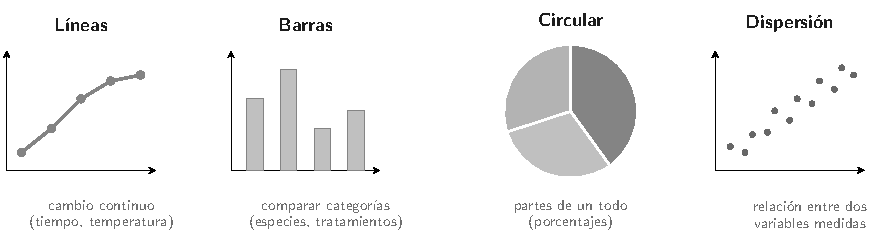
\includegraphics[max width=0.92\linewidth,max height=8.5cm]{bio/hab_graficos}
\end{center}
  
\begin{center}\small
\begin{tabularx}{\linewidth}{@{}>{\raggedright\arraybackslash\hsize=1.31\hsize}X>{\raggedright\arraybackslash\hsize=0.69\hsize}X@{}}
\toprule
\textbf{Objetivo} & \textbf{Recurso} \\
\midrule
Mostrar cómo cambia una variable en el tiempo o con la temperatura & Gráfico de líneas \\
Comparar especies, tratamientos o grupos & Gráfico de barras \\
Mostrar cómo se reparte un total (100 \%) & Gráfico circular \\
Ver si dos variables medidas se relacionan & Gráfico de dispersión \\
Entregar valores exactos o muchas variables & Tabla \\
Mostrar una estructura o un proceso & Esquema o modelo \\
\bottomrule
\end{tabularx}
\end{center}
  
\begin{ejemplo}[{Ejemplo resuelto}] Un equipo mide, en 30 personas, la masa corporal y la cantidad de sangre que bombea el corazón en un minuto. Quiere mostrar si estas variables se relacionan.\par Son dos variables numéricas medidas en cada persona: un \textbf{gráfico de dispersión}, con un punto por persona.\end{ejemplo}
 
\begin{clave}[{Recuerda}] Un buen gráfico tiene título, ejes con nombre y unidad, y la variable independiente en el eje horizontal. El informe de una investigación incluye objetivo, procedimiento, resultados y conclusión.\end{clave}
\subsection{Lo clave del tema}
\begin{center}\small
\begin{tabularx}{\linewidth}{@{}>{\raggedright\arraybackslash\hsize=0.75\hsize}X>{\raggedright\arraybackslash\hsize=1.25\hsize}X@{}}
\toprule
\textbf{Si te piden\dots{}} & \textbf{Revisa esto} \\
\midrule
Evaluar una conclusión & ¿Sale de los datos? ¿Habla solo de lo medido? ¿El diseño permite compararla? \\
El alcance de un estudio & Especie, rango, tipo de muestra y condiciones en que se hizo. \\
Validez & ¿Se midió lo que se quería medir? ¿Hay grupo control? ¿Se controlaron las variables? \\
Confiabilidad & Número de individuos, repeticiones y precisión del instrumento. \\
Mejorar el diseño & La mejora que corrige el defecto que impide responder la pregunta. \\
Resultado o conclusión & Resultado = datos; conclusión = respuesta a la pregunta. \\
Comunicar & El recurso que calza con el objetivo: líneas, barras, circular, dispersión, tabla o esquema. \\
\bottomrule
\end{tabularx}
\end{center}
 
\begin{clave}[{Recuerda}] · Un efecto se atribuye a un tratamiento solo si hay un grupo control comparable.\par · Más individuos de la misma especie y más repeticiones aumentan la confiabilidad.\par · Lo que se mide en células en cultivo o en una especie debe comprobarse antes de aplicarlo a personas o a otras especies.\par · Una asociación entre dos variables no basta para afirmar que una causa la otra.\par · Los datos valen dentro del rango estudiado: fuera de él no se puede afirmar un óptimo ni un valor.\end{clave}
 
\begin{clave}[{Método PAES}] 1. Identifica el objetivo y las variables del estudio. 2. Revisa el diseño: grupo control, variables controladas, número de individuos y repeticiones. 3. Compara la alternativa con los datos y con su rango. 4. Desconfía de «siempre», «todos», «cualquier», «demuestra» y «cura». 5. Si piden comunicar, elige el recurso según lo que se quiere mostrar.\end{clave}
\begin{elejemplo}{PAES Invierno 2026, adaptada}
Unos estudiantes siembran la bacteria \emph{Escherichia coli} en una placa y colocan cuatro discos de papel: tres empapados en los antibióticos A, B y C, y uno (K) empapado solo en agua. Después de 24 horas a 37 °C miden el diámetro de la zona sin bacterias (halo) alrededor de cada disco, como muestra la figura. Con estos datos concluyen: «el antibiótico B es el más eficaz contra todas las bacterias que causan infecciones».

¿Cuál de las siguientes opciones evalúa correctamente esta conclusión?
\begin{center}
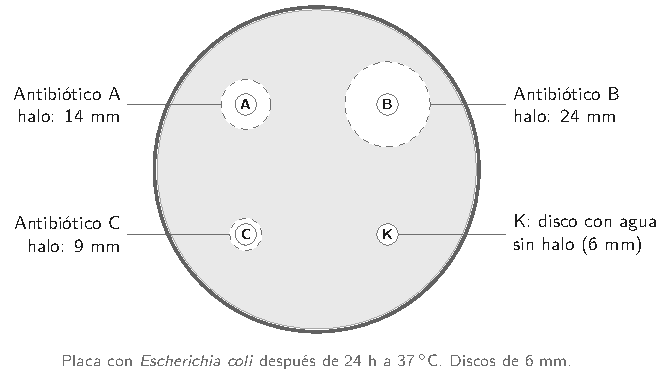
\includegraphics[max width=0.92\linewidth,max height=8.5cm]{bio/hab_antibiotico}
\end{center}
\altslargas{Está respaldada, porque el halo del antibiótico B es el mayor de la placa.}{No está respaldada, porque los datos solo permiten comparar los antibióticos frente a \emph{E. coli}, y se obtuvieron en una sola placa, sin repeticiones.}{No está respaldada, porque el disco K también debió contener un antibiótico.}{Está respaldada, porque el disco K, sin antibiótico, no formó halo.}
\solucion{\textbf{Paso 1. ¿Qué nos piden?} Decidir si la conclusión se sostiene con los datos y con el diseño.

\textbf{Paso 2. ¿Qué muestran los datos?} Halos de 24 mm (B), 14 mm (A), 9 mm (C) y ninguno en K. Contra \emph{E. coli}, en esta placa, el antibiótico B inhibió el crecimiento en la zona más amplia. El disco K muestra que el papel con agua no inhibe a la bacteria.

\textbf{Paso 3. ¿Qué dice la conclusión?} Habla de «todas las bacterias que causan infecciones». Pero se probó \textbf{una sola especie}; otras bacterias pueden responder distinto a cada antibiótico.

\textbf{Paso 4. ¿Y la confiabilidad?} Hay una sola placa y un disco por antibiótico. Para comparar con seguridad se necesitan repeticiones.

\textbf{Respuesta:} no está respaldada, porque los datos solo permiten comparar los antibióticos frente a \emph{E. coli}, y se obtuvieron en una sola placa, sin repeticiones.

\textbf{Una conclusión que sí se sostiene:} «en este ensayo, el antibiótico B produjo el mayor halo de inhibición sobre \emph{E. coli}».

\textbf{¿Por qué no las otras?} «El halo de B es el mayor» es cierto, pero solo para \emph{E. coli}: no justifica hablar de todas las bacterias. «K debió tener antibiótico» se equivoca: K es el grupo control y por eso no debe tenerlo. «K no formó halo» confirma que el control funcionó, pero no resuelve la generalización a otras bacterias.

\textbf{\color{cienciaD}Para recordar.} Una conclusión vale para lo que se probó: la especie, las condiciones y el número de ensayos del estudio.}{B}
\end{elejemplo}
\motivacion{Terminaste Biología y el libro completo: Química, Física y Biología. Los gatitos están muy orgullosos de ti. ¡Ahora a practicar en la página!}
